%*****************************************
\chapter{Introduction}
\label{ch:introduction}
%*****************************************

With the advent of the wave of intelligent and networked vehicles, along with the continuous use of vehicles and smartphones, cloud and big data, especially the continuous innovation of Advanced Driver Assistance System (ADAS) technology, as well as the development of OTA remote upgrade, V2X, information security and other technologies, has propelled the explosive growth in demand for in-vehicle network data transmission capacity\cite{connected_and_Intelligent_Vehicles}.

At present, the mainstream automotive bus technologies mainly include CAN, LIN, FlexRay, CANFD, Automotive Ethernet, etc. CAN bus is still the most widely used in-vehicle bus technology. So a huge amount of automotive CAN bus data is constantly generated and recorded every day. The gathering of CAN bus data allows third parties interested in the automobile ecosystem, such as car manufacturers, repair shops, and road and transportation authorities, to provide continuous support services that promote driver safety while also providing free or pay-as-you-go services\cite{7993938}. This massive amount of vehicle bus data is a valuable asset for enterprises, which can help testing departments monitor vehicle operation in real time and generate reports of various dimensions. And through big data analysis and machine learning, it can make prediction and early warning on vehicle condition, helping enterprises make scientific decisions, save cost and create new value. 

This thesis designs an analysis system based on big data technology for processing and storing CAN bus data. The massive amount of raw binary CAN bus data collected is uploaded to the file system and then filtered and parsed by the big data analysis engine, and the parsed data is stored in the database. Finally, the user can query the required data using SQL. 

\begin{figure}[hbt!]
    \centering
    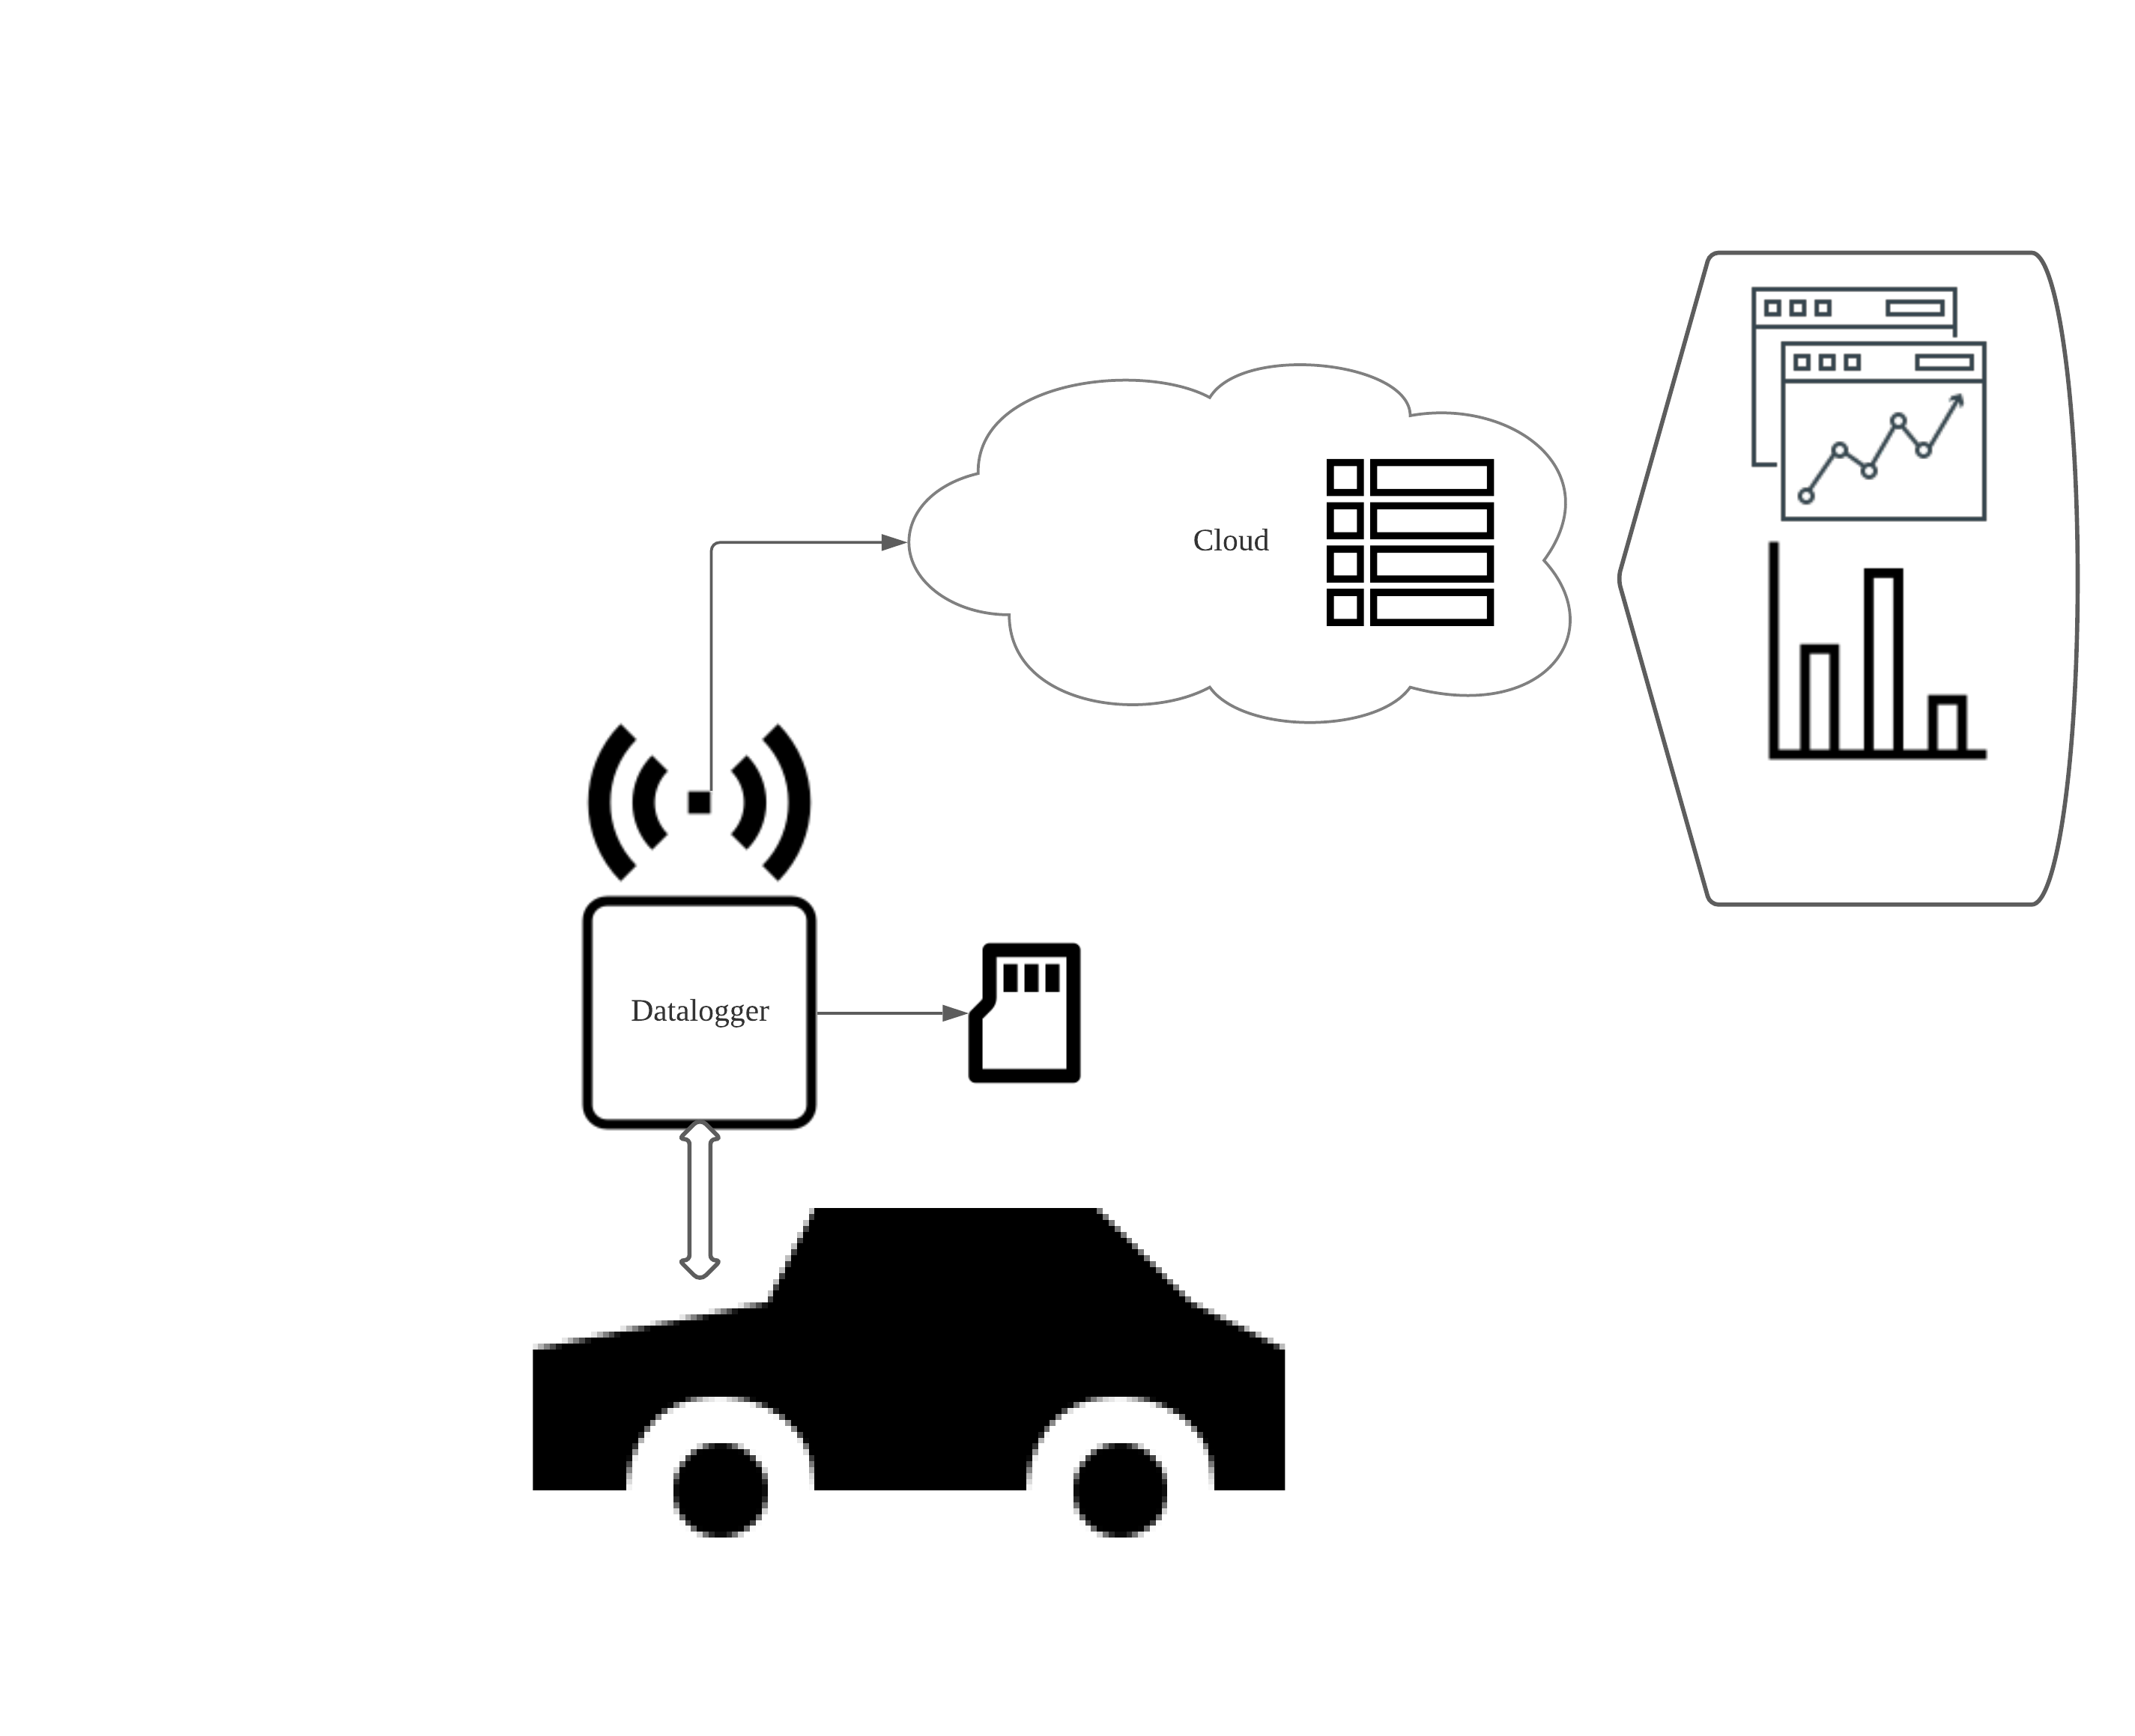
\includegraphics[width=0.5\textwidth]{gfx/zd_datalogger_cloud.png}
    \caption{CAN bus data for visualization}
    \label{fig:galaxy}
\end{figure}

Due to the large number of vehicle bus data records, CAN bus data writing to database becomes a bottleneck, and query analysis is slow. This results in the following essential problem: What are the characteristics of vehicle bus data? How will these massive volumes of car bus data be stored on the server? What kind of database will be able to fulfill the requirements? This question will be explored in further depth throughout the thesis.

The main contribution of this work is that by comparing and analyzing different types of databases in terms of read and write performance, it is concluded that databases with column-oriented and LSM-Tree structure are more suitable for storing CAN bus data, such as ClickHouse, while traditional relational databases, such as MySQL, can also be used as databases for storing CAN bus data, but have many disadvantages.

The following is the outline of this thesis:

\begin{itemize}
    \item Chapter \ref{ch:basics} introduces the foundation of this thesis. First is the basic concept of Big Data and the relationship between Big Data and IoT, followed by data storage and processing techniques. Then comes the basic concept of CAN bus and the characteristics of the data.
    
    \item Chapter \ref{use_case} focuses on the data, including the sources of the data and the information it contains, as well as the use cases of interest to the user. Finally, the functional and non-functional requirements of the user are covered.
    
    \item Chapater \ref{ch:system_architecture} introduces the system architecture, data processing and how the tables in the database are structured.
    
    \item Chapter \ref{ch:choice_of_databases} introduces first the basic structure of data storage for database. Following are four different types of databases, namely MySQL, ClickHouse, Cassandra, and InfluxDB. The characteristics of the databases are analyzed in terms of both the data model and storage engine.
    
    \item Chapter \ref{ch:database_performancecomparison} tests the database mentioned in the previous chapters through several aspects such as write performance, read performance, and disk consumption, and finally summarizes the results.
\end{itemize}

%*****************************************
\chapter{Foundations}
\label{ch:basics}
%*****************************************
The foundations for the thesis are explained in greater depth in this section. The first introduces the basic concepts of Big Data, including the 3Vs and the relationship with IoT. Then this chapter introduces data storage and processing techniques, including HDFS, Spark and database. This thesis focuses on the CAN bus, so the basic concepts of CAN and the characteristics of the data will be mentioned. 


\section{Big Data}
\subsection{Concept}
Big data refers to a collection of data that is so massive or complicated that it is impossible to manage with current database administration tools or standard data-processing software \cite{7888916}. Online transactions, emails, videos, audios, images, sensors, clickstreams, logs, and other sources of data are all used to generate this information\cite[p.~13]{10.5555/2132803}. Big data differs from traditional data analysis in these ways (Figure \ref{fig:big_data}): variety, velocity and volume\cite{6567202}.

\begin{figure}[hbt!]
    \centering
    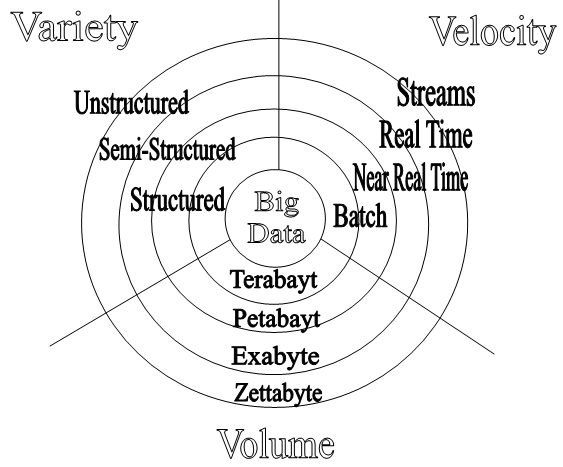
\includegraphics[width=0.3\textwidth]{gfx/big_data.png}
    \caption{3V of Big Data\cite{6567202}}
    \label{fig:big_data}
\end{figure}

\subsection{Volume, Velocity, Variety}

\subsubsection{Volumn}

Terabytes(TB) and petabytes(PB) are inadequate to capture the size of the data. Traditional data storage and analysis techniques are unable to keep up with the scale and growth of data\cite[p.~17]{10.5555/2132803}. One entire genome binary alignment map file, for example, can be over 90 terabytes in size\cite{three_v}. The volume of data that can be processed is limitless, yet the processing pace remains constant. To attain better processing speeds, more computer power is required, which necessitates infrastructure development but at a high expense\cite{tole2013big}.

\subsubsection{Velocity}
"Velocity" refers to the rate at which data flows from point A (which might be an end user interface or a server) to point B (which could have the same characteristics as point A). Typically, data is transferred at a rate that is less than the system's capacity. Because transfer speeds are limited while demands are unbounded, streaming data in real-time or near-real-time is difficult\cite{tole2013big}.

\subsubsection{Variety}

Data acquired by businesses has gotten more complicated as a result of the proliferation of sensors and smart devices, as well as social collaboration platforms\cite{three_v}. Big data is derived from a wide range of sources and is classified into three categories: structured, semistructured, and unstructured\cite[p.~17]{10.5555/2132803}.

\paragraph{Structured data}

Structured data, also known as row data, is defined as data logically expressed and realized by a two-dimensional table structure, strictly adhering to the data format and length specification. It is characterized by: data in rows, a row of data represents the information of an entity, and the attributes of each row of data are the same. Machine language can easily understand structured data because it is well-organized. Those working with relational databases can use a \ac{rdbms} to quickly input, search, and manipulate structured data\cite{structured_data}.

\paragraph{Unstructured data}

Unstructured data is data that is textual in type yet contains a lot of information such as time, numbers, and other variables. Because of their vagueness and non-distinctive nature, they are more difficult to interpret than standard documents in databases or tagged documents. This contains all types of office documents, including text, pictures, XML, HTML, and various reports, photos, and audio/video data, etc. Because unstructured data lacks a predetermined data model, it cannot be organized in relational databases, making it difficult to deconstruct. Non-relational or NoSQL databases, on the other hand, are ideal for handling unstructured data\cite{structured_data}.

\paragraph{Semi-structured data}

Semi-structured data is data that lies between fully structured data (e.g., data in relational databases, object-oriented databases) and completely unstructured data (e.g., sound, image files, etc.). JSON and XML are two instances of semi-structured data. Semi-structured data is more complicated than structured data, but less so than unstructured data. It's also easier to store than unstructured data, bridging the gap between the two sorts of information\cite{structured_data}.


\subsection{Big Data Storage Systems of IoT}
The explosion of data generated by \ac{iot} has had a significant impact on the big data environment. Big data analytics is quickly becoming a crucial IoT initiative for improving productivity. Because significant amounts of data are generated by a large number of dispersed sensors, how to acquire, integrate, store, process, and use this data has become an urgent and crucial problem for businesses to meet their objectives. Engineers are now confronted with the task of processing huge heterogeneous data in highly dispersed situations, particularly in cloud platforms. Perception layer, network layer, and application layer make up a standard IoT application framework\cite{7600359}.


\begin{itemize}
\item Data Acquisition and Integration Module: The data acquisition and integration module collects data from a variety of sensor devices, including RFID, ZigBee sensors, GPS devices, temperature sensors, and so on\cite{7600359}.
\item Data Storage Module: The huge data from sensors consumes a lot of storage space in IoT applications. Meanwhile, data should be compartmentalized for distinct purposes since different roles and tenants require different service and security levels\cite{7600359}. As a result, the primary issues in IoT data storage are how to exchange and isolate this data on cloud platforms.
\item Data Management Module: The data management module creates an intelligent and effective database for IoT applications that are distributed or run in parallel\cite{7600359}. Related works in the field of data management may be divided into three categories: 1) data indexing; 2) semantic annotation; and 3) metadata management.
\item Data Processing Module: MapReduce and its open source implementation Hadoop are two of the most prominent parallel processing algorithms on cloud platforms for parallel or spreading data processing\cite{7600359}. But with the development of time, Spark analytics engine is gradually replacing MapReduce as the most mainstream big data analytics engine\cite{7857034}.
\end{itemize}

\section{Data Storage and processing Technologies}
\subsection{HDFS / Spark}

Normally, the data computed in Spark come from multiple data sources, such as Local File, HDFS, etc. The most common one is HDFS, where users can read large-scale data at one time for parallel computation. After the computation is done, the data can also be stored to HDFS.

\subsubsection{HDFS}

Dataloggers will collect a large amount of raw bus data. Just one server cannot store such a large amount of bus data, so the collected bus data needs to be stored in different servers in a distributed manner. Currently all the bus data is uploaded to the \ac{hdfs} file system.

Hadoop is an open source implementation of Google's Map/Reduce architecture developed by Apache\cite{6558077}. Hadoop stores data using \ac{hdfs}, which is a Google File System (GFS) implementation. HDFS is a distributed file system that runs on commodity hardware. Despite the fact that they have many similarities to current distributed file systems, they are vastly different. HDFS is designed to run on low-cost hardware and has a high level of fault tolerance\cite{179858}. HDFS allows for quick access to application data and is ideal for applications with large data collections.

HDFS cluster is built on a master/slave design, with a single Name Node serving as the master server, managing the file system namespace and controlling client access to files\cite{hadoop_file_system}. The slaves are a group of Data Nodes, generally one for each node in the cluster, that handle storage linked to the nodes on which they operate\cite{6558077}. File system namespace activities such as opening, shutting, and renaming files and directories are performed by the NameNode. It also influences how blocks are mapped to DataNodes. The DataNodes are in charge of servicing the file system's customers' read and write requests. On the NameNode's command, the DataNodes also handle block creation, deletion, and replication\cite{hadoop}.

\begin{figure}[hbt!]
    \centering
    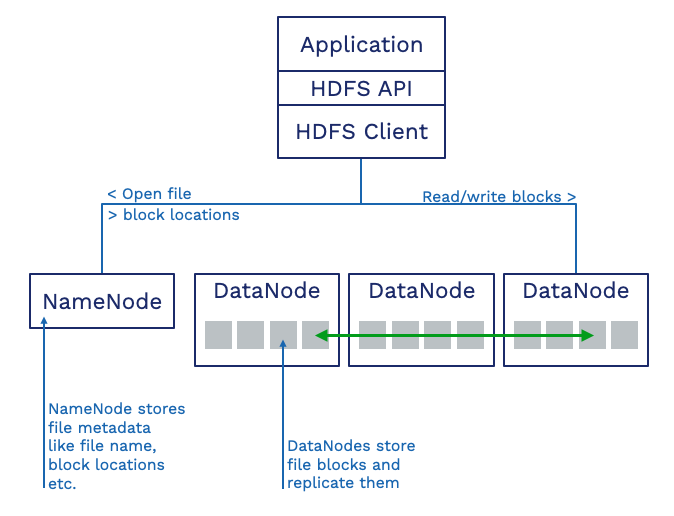
\includegraphics[width=0.5\textwidth]{gfx/hdfspng.png}
    \caption{HDFS Architecture\cite{HDFS_Architecture}}
    \label{fig:hdfs_architecture}
\end{figure}

\subsubsection{Spark}

Apache Spark is a large-scale data processing engine with a unified analytics engine. It includes Java, Scala, Python, and R high-level APIs, as well as an efficient engine that supports broad execution graphs. With in-memory computing, Spark is faster than Hadoop. Spark SQL for SQL and structured data processing, MLlib for machine learning, GraphX for graph processing, and Structured Streaming for incremental computing and stream processing are among the higher-level technologies it offers\cite{spark2018apache}.

\begin{itemize}
    \item Spark SQL: 
    
    Spark SQL is a module used by Spark to process structured data. It provides 2 programming abstractions: DataFrame and DataSet, and acts as a distributed SQL query engine\cite{10.1145/2723372.2742797}.
    
    \item RDD
    
    \ac{rdd} is the fundamental data structure of Spark and it is the primary data abstraction in Spark. RDDs are fault-tolerant, immutable distributed collections of things, meaning they can't be changed after they've been created. RDD divides each dataset into logical partitions that can be computed on separate cluster nodes\cite{rdd}.
    
    \item Dataframe: 
    
    Similar to \ac{rdd}, the Dataframe is a distributed data container. However, DataFrames are more like traditional databases with two-dimensional tables\cite{10.1145/2723372.2742797} that record structural information about the data, i.e. schema.
    
\end{itemize}

\subsubsection{Scala}
Scala is a hybrid functional programming language. It combines elements of object-oriented and functional programming. Every value is treated as an object in this Object Oriented Programming Language\cite{scala_documentation}. Scala programs can be converted to bytecodes and run on the \ac{jvm}. It defines anonymous functions, higher-order functions, and nested functions as a functional programming language\cite{geeksforgeeks_2021}. Scala is one programming language that is used to write Spark.

Apache Spark code will be written with the Scala in this thesis. Scala programming language is 10 times faster than Python for data analysis and processing due to JVM. The performance is mediocre when Python programming code is used to make calls to Spark libraries but if there is lot of processing involved than Python code becomes much slower than the Scala equivalent code\cite{9315863}.

\subsection{Database}
A database is a collection of data structures that can be used to organize, store, and manage data. It is an organized, shareable, and uniformly managed collection of large amounts of data stored within servers over a long period of time\cite{wikipedia_database}.

\subsubsection{Relational Databases}

The relational model, an intuitive and simple way of representing data in tables, is the foundation of relational databases. Each row of a table in a relational database is a record with a unique identifier known as the key. The attributes of the data are stored in the table's columns, and each record usually has a value for each attribute, making it simple to connect data points.

Tables in relational databases store a number of formatted data structures, with each tuple field having the same composition. Even though not all fields are needed for each tuple, the database assigns all fields to each tuple, which makes it easier to perform operations such as joins between tables, but on the other hand it is also a performance bottleneck in relational databases.

\begin{figure}[hbt!]
	\centering
 	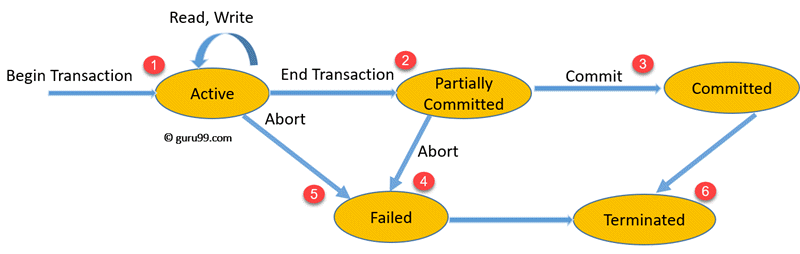
\includegraphics[width=0.5\textwidth]{gfx/DBMSTransac.png}  	  	 	
	\caption{ACID\cite{peterson_2021}}
	\label{fig:acid}
\end{figure}

\begin{itemize}
    \item Database Transaction
    
    When executing SQL statements, certain requirements dictate that a series of operations must be executed in full, not just in part, for example, a transfer operation. The database transaction ensures that all operations within the scope of that transaction can either all succeed or all fail. If the transaction fails, then the effect is the same as if the SQL had not been executed, and no changes are made to the database data. ACID Properties are utilized to keep the database's integrity throughout transaction processing\cite{peterson_2021}.
    
    \begin{enumerate}
        \item Atomicity: Execute all SQL as atomic units of work, either all or none.
        
        \item Consistency: The state of all data is consistent after the transaction completes. 
        
        \item Durability: If there are multiple transactions executing concurrently, the changes made by each transaction must be isolated from the other transactions.
        
        \item Isolation: After the transaction is completed, modifications to the database data are stored persistently.
    \end{enumerate}
\end{itemize}

\subsubsection{Non-Relational Databases}

Unlike relational databases, non-relational databases(NoSQL) do not store data in the form of tables and records. Instead, in these types of databases, the data storage structure is designed and optimized for specific requirements. NoSQL presents an alternative notion, such as storing in key-value pairs with a non-fixed structure, where each tuple can have various fields and each tuple can add part of its own key-value pairs as needed, to avoid being bound by a predefined structure and to save time and space\cite{menegasso_2018}. Column-store databases, document-based databases, key-value databases, and graph databases are the four most common forms of NoSQL databases. These types can be used individually or in combination. NoSQL databases typically have the following characteristics:

\begin{itemize}
    \item No relational data model
    
    \item Weak schema restrictions
    
    \item No ACID transaction model
    
    \item Simple data replications
    
    \item Horizontal scalability
\end{itemize}

\begin{table}[hbt!]
\centering
\resizebox{\textwidth}{!}{%
\begin{tabular}{@{}l|l|l@{}}
\toprule
 &
  \textbf{Relational databases} &
  \textbf{NoSQL databases} \\ \midrule
\textbf{Data model} &
  {\color[HTML]{333333} \begin{tabular}[c]{@{}l@{}}The relational model normalizes data into tables that are composed\\ of rows and columns. A schema strictly defines the tables, rows,\\ columns, indexes, relationships between tables, and other database\\ elements. The database enforces the referential integrity in \\ relationships between tables.\end{tabular}} &
  \begin{tabular}[c]{@{}l@{}}NoSQL databases provide a variety of data models such as key-value, \\ document, and graph, which are optimized for performance and scale.\end{tabular} \\ \midrule
\textbf{\begin{tabular}[c]{@{}l@{}}ACID \\ properties\end{tabular}} &
  \begin{tabular}[c]{@{}l@{}}Relational databases provide atomicity, consistency, isolation,\\ and durability (ACID) properties.\end{tabular} &
  \begin{tabular}[c]{@{}l@{}}NoSQL databases often make tradeoffs by relaxing some of the ACID properties \\ of relational databases for a more flexible data model that can scale \\ horizontally. This makes NoSQL databases an excellent choice for high \\ throughput, low-latency use cases that need to scale horizontally beyond\\ the limitations of a single instance.\end{tabular} \\ \midrule
\textbf{Performance} &
  \begin{tabular}[c]{@{}l@{}}Performance is generally dependent on the disk subsystem. \\ The optimization of queries, indexes, and table structure is \\ often required to achieve peak performance.\end{tabular} &
  \begin{tabular}[c]{@{}l@{}}Performance is generally a function of the underlying hardware \\ cluster size, network latency, and the calling application.\end{tabular} \\ \midrule
\textbf{Scale} &
  \begin{tabular}[c]{@{}l@{}}Relational databases typically scale up by increasing the \\ compute capabilities of the hardware or scale-out by \\ adding replicas for read-only workloads.\end{tabular} &
  \begin{tabular}[c]{@{}l@{}}NoSQL databases typically are partitionable because access patterns \\ are able to scale out by using distributed architecture to increase \\ throughput that provides consistent performance at near boundless \\ scale.\end{tabular} \\ \bottomrule
\end{tabular}%
}
\caption{Relational databases vs NoSQL databases\cite{menegasso_2018}}
\label{tab:rdbvsnosql}
\end{table}

\subsubsection{OLTP vs OLAP}

Data processing can be broadly divided into two categories: \ac{oltp} and \ac{olap}. Traditional relational databases' primary application is OLTP, which focuses on basic, routine transactions like bank transactions, whereas data warehousing systems' primary application is OLAP, which supports complex analytical operations, focuses on decision support, and provides intuitive and easy-to-understand query results\cite{birost}. 

The main differences between OLTP and OLAP are:

\begin{itemize}
    \item OLTP is the main application of traditional relational databases, mainly for basic, daily transactions, recording immediate additions, deletions, changes and checks, such as accessing a sum of money in a bank, which is a transaction transaction; OLAP is the core of data warehousing, supporting complex analytical operations, focusing on decision support, and providing intuitive and easy-to-understand query results. A typical application is a complex dynamic reporting system.
    
    \item Real-time requirements of OLTP  are high, OLTP database is designed to enable transactional applications to write only the data needed to process a single transaction as quickly as possible. In contrast real-time requirements of OLAP are not very high.
    
    \item OLTP uses ER model and application-oriented database design. OLAP uses star or snowflake model and subject-oriented database design\cite{ibm_oltp}.
    
    \item OLTP data volume is not very large, generally only read/write dozens of records, processing simple transactions. OLAP data volume is large, because OLAP support is dynamic query, so the user may have to through will be a lot of data after the statistics to get the information you want to know, such as time series analysis and so on, so processing a large amount of data\cite{ibm_oltp}.

    \item OLTP systems change data regularly, whereas OLAP systems do not.
\end{itemize}

\section{CAN Bus data}
Bosch created the \ac{can} serial bus communications protocol in the early 1980s. It establishes a standard for efficient and dependable communication in real-time applications between sensors, actuators, controllers, and other nodes\cite{4677544}. Most vehicle manufacturers use the CAN high-speed network for powertrain communication, with transmission rates ranging from 125kb/s to 1Mb/s. 

\subsection{Basic principles of CAN bus}
CAN bus is a broadcast type of bus, so this means all nodes can “hear” all transmissions\cite{can_protocol}. The data information sent by any node does not include the physical address of the sending or receiving node. The data is marked by an identifier (ID), which is unique throughout the network. After receiving the message, other nodes detect this identifier to determine whether to process. The smaller the CAN-ID value, the higher its priority. This method is called Multi-master priority based protocol. 

\subsubsection{CAN Physical Layers}
The CAN bus follows the ISO/OSI model and defines the data link layer and physical layer of the OSI model. The physical layer is the circuitry that enables the ECU to be connected to the bus. The signals are transmitted using differential voltages, called CAN\_H and CAN\_L. When both are 2.5V, this state is logically 1 (recessive). When CAN\_H is higher than CAN\_L, it indicates logically 0 (dominant).

Non-Return To Zero (NRZ) with bit-stuffing is used on the CAN bus. Signaling states have two logical values, dominant and recessive. As long as a node drives the bus to the dominant state, the entire bus is in that state regardless of how many nodes transmit the recessive state\cite{can_protocol}.

\subsubsection{CAN Messages}
CAN messages are divided into four different types according to their use:
\begin{enumerate}
    \item Data frame: Transferring data
    \item Remote Frame: Request to send data
    \item Error Frame: Identify detected errors
    \item Overload Frame: Delay the sending of the next message frame
\end{enumerate}

\begin{figure}[hbt!]
    \centering
    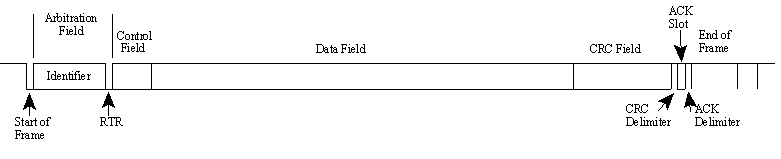
\includegraphics[width=0.6\textwidth]{gfx/data_framepng.png}
    \caption{Data Frame\cite{can_protocol}}
    \label{fig:data_frame}
\end{figure}

\subsubsection{DBC file}
Vector Informatik GmbH created the \ac{dbc} in the 1990s to provide a standard way of storing information described in a CAN network. DBC files become the accepted standard for exchanging CAN descriptions, mainly in the automotive industry. The DBC file is an ASCII-based translation file that is used to apply identifying names, scaling, offsets, and defining information to data sent over the CAN bus. A DBC file can identify any or all of the data within a CAN frame for any given CAN ID\cite{kvaser_2021}.

\begin{figure}[hbt!]
\centering
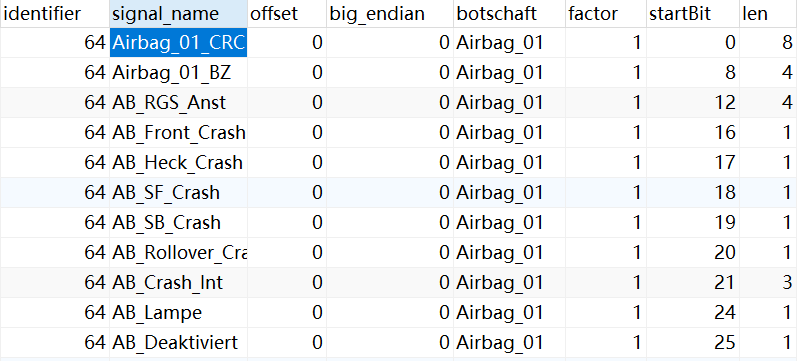
\includegraphics[width=0.5\textwidth]{gfx/dbc_database.png}
\caption{DBC rule in database}
\label{fig:dbc_rule}
\end{figure}

\subsection{The characteristics of the CAN bus data}

CAN data frames are recorded during the test drives in the vehicle with the help of ZD-Dataloggers. The raw CAN bus data is incomprehensible to humans. See table \ref{tab:raw_canbus}. The DBC file is a basic text file that contains data for decoding raw CAN bus data to physical values or human readable form. Parameters (signals) can be "extracted" from data bytes using a CAN DBC with CAN ID decoding rules. The data after parsing according to the DBC file is shown in the table \ref{tab:parsing_canbus} below.


\begin{table}[hbt!]
\centering
\begin{tabular}{@{}ccl@{}}
\toprule
\textbf{Timestamp} & \textbf{ID} & \multicolumn{1}{c}{\textbf{Data bytes}} \\ \midrule
1601199986095518   & 663         & 70 28 01 0E 00 89 00 04                 \\
1601199986099540   & 3C0         & 4C 00 07 00                             \\
1601199987003519   & 6B4         & 02 39 30 35 30 33 30 32                 \\ \bottomrule
\end{tabular}
\caption{Raw CAN Bus data}
\label{tab:raw_canbus}
\end{table}


\begin{table}[hbt!]
\centering
\resizebox{\textwidth}{!}{%
\begin{tabular}{@{}ccl@{}}
\toprule
\textbf{Timestamp} &
  \textbf{ID} &
  \multicolumn{1}{c}{\textbf{Data bytes}} \\ \midrule
1601199986095518 &
  663 &
  \begin{tabular}[c]{@{}l@{}}\{NM\_Gateway\_NM\_aktiv\_Tmin -\textgreater 1, NM\_Gateway\_SNI -\textgreater 16, NM\_Gateway\_NM\_aktiv\_Connect -\textgreater 1, NM\_Gateway\_CBV\_AWB -\textgreater 1,\\  NM\_Gateway\_Car\_Wakeup -\textgreater 0, NM\_Gateway\_NM\_aktiv\_OBDC -\textgreater 0, NM\_Gateway\_NM\_aktiv\_FC -\textgreater 0, NM\_Gateway\_NM\_aktiv\_KL15 -\textgreater 0,\\  NM\_Gateway\_CBV\_CRI -\textgreater 1, NM\_Gateway\_UDS\_CC -\textgreater 0, NM\_Gateway\_CAB -\textgreater 16515369, NM\_Gateway\_NM\_aktiv\_Diagnose -\textgreater 0,\\  NM\_Gateway\_NM\_aktiv\_EM -\textgreater 0, NM\_Gateway\_NM\_State -\textgreater 1, NM\_Gateway\_NM\_aktiv\_CWU -\textgreater 1\}\end{tabular} \\ \hline
1601199986099540 &
  3C0 &
  \begin{tabular}[c]{@{}l@{}}\{Gateway\_Transport\_Mode -\textgreater 0, Gateway\_SNI -\textgreater 16, NM\_Gateway\_Subsystemaktiv -\textgreater 0, Gateway\_Matrix\_Generation -\textgreater 2,\\  GW\_KD\_Fehler -\textgreater 1, Gateway\_KompSchutz -\textgreater 0, Gateway\_Abschaltstufe -\textgreater 0, NM\_Gateway\_Wakeup -\textgreater 131, \\ Gateway\_Matrix\_Version -\textgreater 19, Gateway\_Nachlauftyp -\textgreater 2, NM\_Gateway\_Lokalaktiv -\textgreater 0\}\end{tabular} \\ \hline
1601199987003519 &
  6B4 &
  \begin{tabular}[c]{@{}l@{}}\{APS\_Taster -\textgreater 2, APS\_LED\_Status -\textgreater 0, LIM\_PAO\_ON\_Status -\textgreater 0, PLA\_LED\_Status -\textgreater 0, AVH\_Taster -\textgreater 0, Heckrollo\_Taster -\textgreater 2,\\  Display\_Taster -\textgreater 2, LIM\_PAO\_OFF\_Status -\textgreater 0, Spoiler\_Taster -\textgreater 2, Heckrollo\_2\_Taster -\textgreater 2, PLA\_Taster\_Fehler\_Roh -\textgreater 0,\\  Sideview\_Taster -\textgreater 2, Drivesel\_1\_Taster -\textgreater 2, Drivesel\_2\_Taster -\textgreater 2, ESP\_Off\_Taster -\textgreater 2, LIM\_PAO\_Schriftzug\_Status -\textgreater 0, \\  AVH\_LED\_Status -\textgreater 0, eCall\_Taste -\textgreater 0, HDC\_LED\_Status -\textgreater 0, PLA\_Taster -\textgreater 2, SWA\_Taster -\textgreater 2, LIM\_bCall\_Taster -\textgreater 0,\\  LKS\_Taster -\textgreater 2, Spoiler\_LED\_Status -\textgreater 0, LIM\_PAO\_Alivesignal -\textgreater 0, HDC\_Taster -\textgreater 2\}\end{tabular} \\ \bottomrule
\end{tabular}%
}
	\caption{Data after parsing according to CAN DBC file}
	\label{tab:parsing_canbus}
\end{table}

The following features apply to the parsed CAN bus data.

\begin{description}
\item[Time-series data]: For computation or analysis, the timestamp associated with each data record is crucial. Timestamps are used to index the data records\cite{taos_data}.
\item[Structured data]: Each data with the same CAN ID has a predefined data type or fixed length. For example, the data from CAN ID 64 is shown in the table \ref{tab:CAN_IDA64} below.
\item[Large amount of data]: A Datalogger can collect up to 300GB of car data per day. About 10 GB of this data is CAN bus data. Currently there are about 10 devices that are responsible for collecting the data. That means that 100GB with about 2 billion rows of CAN bus data will be available every day.
\item[No updates on data]: The CAN bus data stored in the database is generally not necessary to be modified.
\item[Aggregation over time or a set of devices]: The majority of queries are run on a specific time period, rather than all of the historical data.
\item[Retention policy]: The data is not required to be kept permanently. When the life cycle of the data ends, the data will be deleted.
\item[The trend is crucial]: Users prefer to pay attention to CAN bus data trends within a certain time range, such as the past 10 minutes or 1 hour.
\item[Real-time calculations or analysis necessary]: such as vehicle speed, startup speed or vehicle interior temperature.
\end{description}

\begin{table}[hbt!]
\centering
\resizebox{\textwidth}{!}{%
\begin{tabular}{@{}ccl@{}}
\toprule
\textbf{Timestamp} & \textbf{ID} & \multicolumn{1}{c}{\textbf{Data bytes}} \\ \midrule
1601199986095518 & 64 & {[}50, 9, 0, 0, 0, 0, 0, 0, 0, 1, 0, 0, 0, 0, 0, 0, 1, 0, 0, 0, 0, 0, 0, 0, 0, 0, 0, 0, 39{]}   \\
1601199986099540 & 64 & {[}22, 10, 0, 0, 0, 0, 0, 0, 0, 1, 0, 0, 0, 0, 0, 0, 1, 0, 0, 0, 0, 0, 0, 0, 0, 0, 0, 0, 40{]}  \\
1601199987003519 & 64 & {[}143, 11, 0, 0, 0, 0, 0, 0, 0, 1, 0, 0, 0, 0, 0, 0, 1, 0, 0, 0, 0, 0, 0, 0, 0, 0, 0, 0, 41{]} \\ \bottomrule
\end{tabular}%
}
\caption{Data with CAN ID 64}
\label{tab:CAN_IDA64}
\end{table}

Compared to traditional Internet data, the volume of automotive bus data is larger and the speed of writing is therefore more important. Internet data is more unstructured data, such as ebay's transaction records, but CAN bus data is all time-series and structured. There are different data processing requirements compared to Internet data. For example, the total amount of data for a particular CAN ID in one second is too much, so a downsampling query is needed.

\section{Related Work}

\subsection{Reference Architectures}
There is very little research on big data storage designed specifically for the CAN bus, and I have found only one solution so far.

Jong-Wook Jang\cite{7993938} has designed a system architecture based on MapReduce and Hadoop for querying CAN bus data. The system architecture is shown in the Figure \ref{fig:jong} below. The framework analytical model is expressed as a function that takes input from the HDFS and converts it into MapReduce jobs once the HiveQL scripts are run. The analysis continues to separate the CAN bus data based on events in the Engine Control Units (ECU), and then selects the key value pairs to include in the input function that is sent to the Hadoop\cite{7993938}.

\begin{figure}[hbt!]
    \centering
    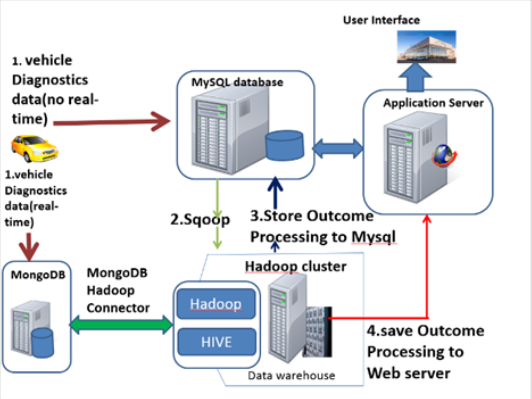
\includegraphics[width=0.5\textwidth]{gfx/jong.png}
    \caption{Processing CAN-Bus data using Hadoop and MapReduce\cite{7993938}}
    \label{fig:jong}
\end{figure}

The disadvantage of this architecture is that the CAN bus cannot be queried in real time, and the stored CAN bus data is only a filtered portion. By analyzing Jang's system architecture, I redesigned the system architecture from how CAN bus data is stored, parsed, and loaded into the database, making the whole system more suitable for real-time analysis. 



\subsection{Database Benchmarks}
Benchmarking database performance is a science in and of itself, and it's difficult to acquire consistent and comparable results. Database benchmarking is a well-established and well-defined approach for analyzing and comparing database performance characteristics. The general understanding of benchmarking is to measure and compare various performance dimensions with different practical solutions based on a well-defined methodology. Portfolios or diagrams are commonly used to present the outcomes. The goal of benchmarking is to build a continuous improvement process\cite{benchmarking}.

The 4 steps of the general benchmarking framework:
\begin{enumerate}
    \item Define model by setting a goal, the process and constraints.
    \item Identify related entities, resources, artefacts and data.
    \item Measure or calculate all options.
    \item Compare the results with the identified benchmark\cite{benchmarking}.
\end{enumerate}

~\\
This thesis refers to the Time Series Benchmark Suite (TSBS)\cite{tsbs}, a specialized benchmarking for time series databases. TSBS is used to benchmark bulk load performance and query execution performance. Using TSBS for benchmarking involves three phases: data and query generation, data loading and query execution. In the IoT use case of TSBS, a data stream of a set of trucks from a trucking company is simulated, including various diagnostic data and metrics as well as environmental factors\cite{tsbs}. The truck status is then analyzed in real time through database query operations. This is very similar to our case of collecting CAN bus data, parsing the data and writing it to the database, and then querying the required information in real time.


%*******************************************
\chapter{Use Cases}
\label{use_case}
The querying model is based on a data-driven approach. Since the database stores the data of all CAN-IDs involved in the DBC file, users can get data of different aspects of activity of the vehicles according to their needs via sql.
This chapter introduce the required data, use case and requirements from users.

\section{Required data}
The raw CAN bus data is stored in binary form (Figure \ref{fig:raw_data}) and is collected from the car via ZD-Dataloggers. The data required for this thesis are from the Audi A8 model and distributed over different time periods. The collected CAN bus types are drive train and infotainment. According to the DBC file of Audi a8, the total number of CAN-IDs is 520 (Figure \ref{fig:can_idtable}), which belong to different control units.

\begin{figure}[hbt!]
    \centering
    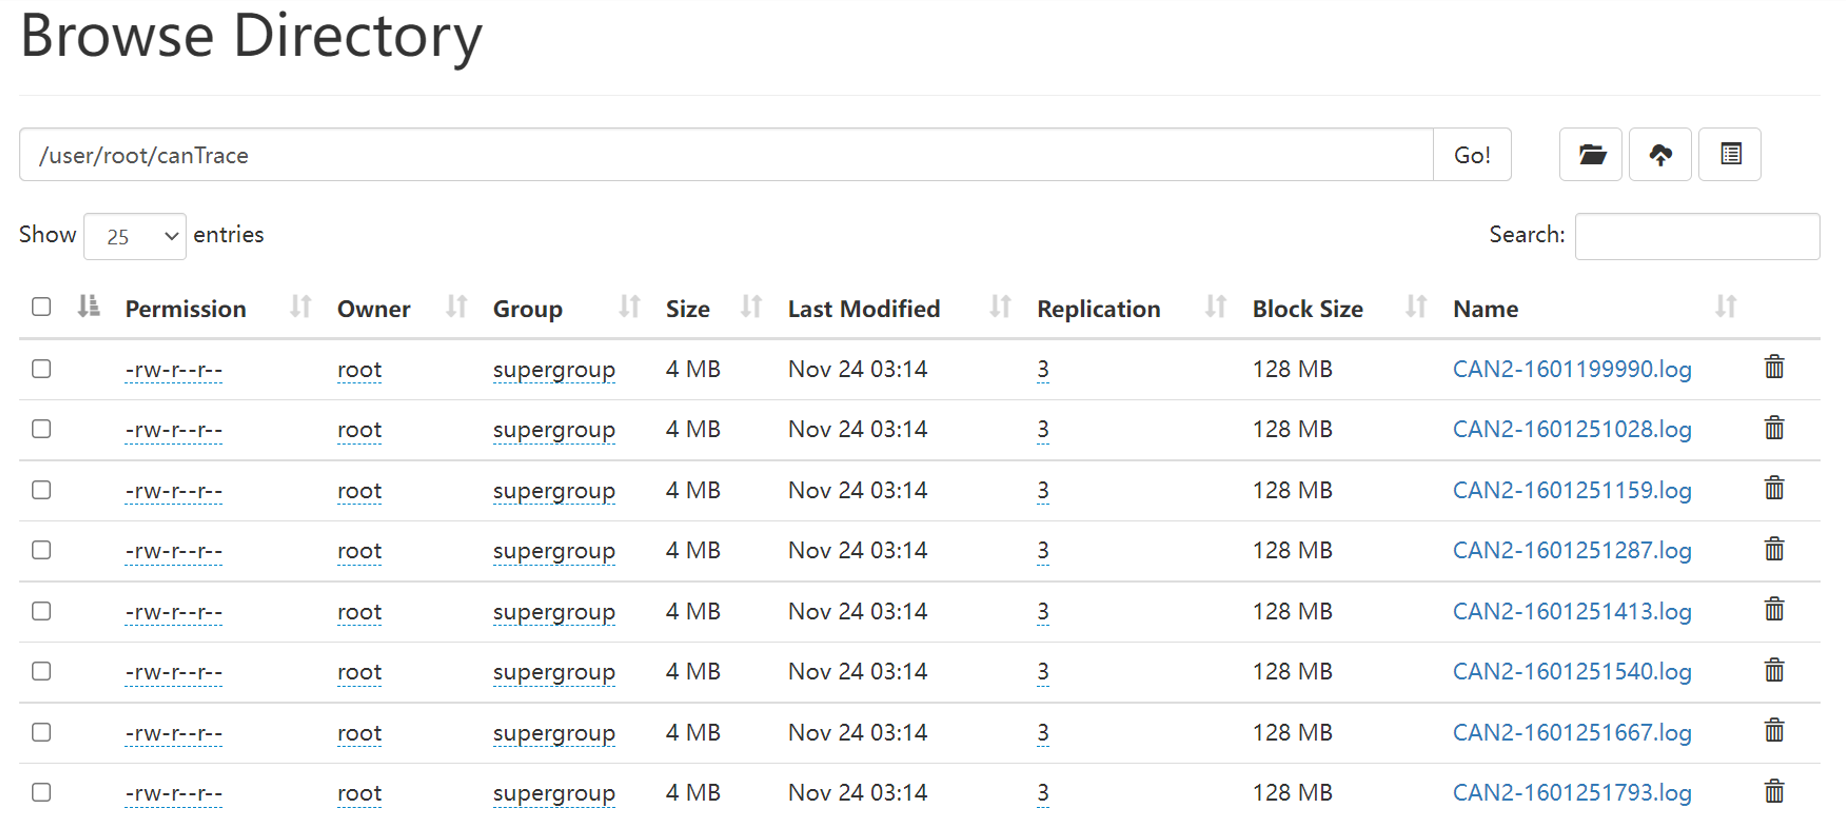
\includegraphics[width=0.8\textwidth]{gfx/raw_data.png}
    \caption{Raw-CAN DATA}
    \label{fig:raw_data}
\end{figure}

The CAN drive data bus control units are as follows:
\begin{itemize}
    \item Motor control unit
    \item \ac{abs}-Control Unit
    \item \ac{esp}-Control Unit
    \item Transmission Control Unit
    \item Airbag Control Unit
    \item Combined instrumentation
\end{itemize}

The CAN infotainment bus control units are as follows:
\begin{itemize}
\item Air conditioning control unit
\item Door control unit
\item Comfort Control Unit
\item Radio and navigation display control unit
\end{itemize}



\section{Use Case Overview}
The user queries the CAN bus data in real time according to the time period. In general, the user will be more interested in newer data, such as yesterday's or today's data. The time range of the query is usually a few minutes, a few hours or a whole day. In addition,  sometimes filter conditions are attached. The main queries are divided into the following categories and examples will be shown in \ac{sql} form.

\begin{enumerate}
    \item The user downloads all or part data for certain CAN-IDs for certain time periods and stores it in CSV or other file formats. These data can be used for further analysis using tools such as CANOE. 
    
    
    \begin{minted}[
frame=lines,
framesep=2mm,
baselinestretch=1.2,
bgcolor=LightGray,
fontsize=\footnotesize,
linenos
]{bash}
# Query all the data of CAN_ID of Airbag_01 for certain periods of time
SELECT * FROM audi_a8.Airbag_01 
WHERE ts BETWEEN '2021-11-05 08:00:00' AND '2021-11-05 12:00:00' 
OR ts BETWEEN '2021-11-06 08:00:00' AND '2021-11-06 12:00:00'
-format CSV > motor_12_ch.csv

# Query the data of CAN_ID of Airbag_01 for certain periods of time with the filter
SELECT * FROM audi_a8.Airbag_01
WHERE ts BETWEEN '2021-11-05 08:00:00' AND '2021-11-05 12:00:00'
AND AB_VB_deaktiviert = 1
-format CSV > motor_12_ch.csv
\end{minted}
    
    \item The user uses \ac{sql} aggregation to query a specific data of a certain CAN-ID, such as the average speed of the car engine, the minimum temperature inside the car or the maximum value of the car's acceleration for a certain period of time. 
    
        \begin{minted}[
frame=lines,
framesep=2mm,
baselinestretch=1.2,
bgcolor=LightGray,
fontsize=\footnotesize,
linenos
]{bash}
# Query the average temperature of the A/C sensor for the past three hours
SELECT avg(FS_Temp_Sensor) 
FROM audi_a8.Klima_Sensor_01
WHERE ts BETWEEN subtractHours(now(), 3) and now()
--------------------------------------------------------------------------------------------------
┌─avg(FS_Temp_Sensor)─┐
│  140.75292864749733 │
└─────────────────────┘
# Query the maximum and minimum temperature and timestamp of the A/C sensor for the past three hours
SELECT ts,  FS_Temp_Sensor 
FROM audi_a8.Klima_Sensor_01,
(SELECT max(FS_Temp_Sensor) AS maxTemp, min(FS_Temp_Sensor) AS minTemp
FROM audi_a8.Klima_Sensor_01 
WHERE ts BETWEEN subtractHours(now(), 3) and now()
) AS tmp
WHERE FS_Temp_Sensor = tmp.maxTemp OR FS_Temp_Sensor = tmp.minTemp
--------------------------------------------------------------------------------------------------
┌─────────────────────────ts─┬─            FS_Temp_Sensor─┐
│ 2021-09-27 10:48:58.078129│              0 │
│ 2021-09-28 00:17:37.028350 │           164 │
\end{minted}
    


\item Implement the function of decreasing the data collection frequency (downsampling). The data interval of various CAN-IDs is different, for example, the signal interval of car speed is very short, usually only a few milliseconds. In some cases, such as data visualization, the user does not need so much data and wants to count at the frequency of seconds or minutes, so the amount of data can be greatly reduced.

        \begin{minted}[
frame=lines,
framesep=2mm,
baselinestretch=1.2,
bgcolor=LightGray,
fontsize=\footnotesize,
linenos
]{bash}
# Query the average value of rpm of motor per minute
SELECT time,
       avg(MO_Drehzahl_01)
FROM audi_a8.Motor_12
WHERE ts BETWEEN subtractHours(now(), 3) and now()
GROUP BY toStartOfMinute(ts) AS time
ORDER BY second

# After downsampling, data from several different CAN_ID tables are joined according to time
# Average of RPM of motor and temperature sensors per minute over a period of time
SELECT motor.minute AS time,motor.avg_rpm, ac.avg_temp
FROM
(SELECT minute, avg(MO_Drehzahl_01) AS avg_rpm
FROM audi_a8.Motor_12
WHERE ts BETWEEN subtractHours(now(), 3) and now()
GROUP BY toStartOfMinute(ts) AS minute
ORDER BY minute
) AS motor
JOIN
(SELECT minute, avg(FS_Temp_Sensor) AS avg_temp
FROM audi_a8.Klima_Sensor_01
WHERE ts BETWEEN subtractHours(now(), 3) and now()
GROUP BY toStartOfMinute(ts) AS minute
ORDER BY minute
) AS ac
ON motor.minute = ac.minute

--------------------------------------------------------------------------------------------------
┌────────────────time─┬────────────avg_rpm─┬───────────avg_temp─┐
│ 2021-09-27 05:46:00 │                  0 │                132 │
│ 2021-09-27 05:47:00 │                  0 │  132.1153846153846 │
│ 2021-09-27 05:48:00 │  2409.159060011653 │                133 │
\end{minted}

\item Calculate the difference between successive row of the column elements. For example, the trend of \ac{gps} change or the change of car mileage.

        \begin{minted}[
frame=lines,
framesep=2mm,
baselinestretch=1.2,
bgcolor=LightGray,
fontsize=\footnotesize,
linenos
]{bash}
# Query the difference between successive row values of GPS longitude and latitude
SELECT 
    ts,
    runningDifference(NP_LatDegree),
    runningDifference(NP_LongDegree)
FROM audi_a8.NavPos_01
WHERE ts BETWEEN '2021-09-27 08:00:00' AND '2021-09-28 22:00:00'
--------------------------------------------------------------------------------------------------
┌─────────────────────────ts─┬─runningDifference(NP_LatDegree)─┬─runningDifference(NP_LongDegree)─┐
│ 2021-09-27 05:46:27.007512 │                               2 │                                -2 │
│ 2021-09-27 05:46:27.027678 │                               1 │                                0 │
│ 2021-09-27 05:46:27.047343 │                               3 │                                -2 │
└────────────────────────────┴─────────────────────────────────┴──────────────────────────────────┘
# Combine downsampling and calculate the change per second
SELECT
  time,
  runningDifference(NP_LatDegree) AS delta_Lat,
  runningDifference(NP_LongDegree) AS delta_Long
FROM
  (
    SELECT
      time,
      avg(NP_LatDegree) AS NP_LatDegree,
      avg(NP_LongDegree) AS NP_LongDegree
    FROM
      audi_a8.NavPos_01
    GROUP BY
      toStartOfSecond(ts) AS time
    ORDER BY
      time
  )
 --------------------------------------------------------------------------------------------------
┌───────────────────────time─┬─delta_Lat─┬─delta_Long─┐
│ 2020-09-27 05:46:27.000000 │         6 │          -51 │
│ 2020-09-27 05:46:28.000000 │         58 │         -172 │
│ 2020-09-27 05:46:29.000000 │         97 │         -190 │
\end{minted}

\end{enumerate}

\section{Requirements}
Requirements analysis is a crucial process for determining the success of a system. Functional and non-functional requirements are the most common types of requirements. Functional Requirements are the basic features that the system should provide that the user specifically requests. Non-functional requirements are basically the quality constraints that the system must satisfy\cite{geeksforgeeks_2020}. 

By asking the engineers in the company, the following requirements are summarized.

\begin{itemize}
    \item Functional Requirement
    
    \begin{enumerate}
        \item Large amounts of raw data need to be stored in a distributed system.
        \item The user is able to write a large amount of CAN bus data into the database.
        \item The user can query data according to CAN-ID and time period via \ac{sql}.
        \item The user can perform fast aggregation operations on certain columns of data.
        \item The user can aggregate the collected data by time period by downsampling.
        \item The database supports distributed storage.
        \item The database must be open source.
    \end{enumerate}
    
    \item Non-functional Requirement
\begin{enumerate}
    \item Continuous and stable writes: 
    
    The writing speed of the system must be greater than 50,000 lines per second.
    \item Systems for Real-Time Processing:
    
    Users need to do real-time warning and decision making based on the collected data, and the latency should be controlled within seconds.
    \item High compression rate:
    
    The data stored in the database cannot be larger than the original file
    \item Scalability:
    
    The system can quickly add or delete nodes.
\end{enumerate}
\end{itemize}


%*****************************************
\chapter{System architecture}
\label{ch:system_architecture}
%*****************************************
By analyzing the Use Case in the previous chapter, the requirements of the user can be obtained. This chapter describes the system architecture, data processing and how the tables in the database are structured. 

\section{Implementation steps of the system}

\begin{figure}[hbt!]
    \centering
    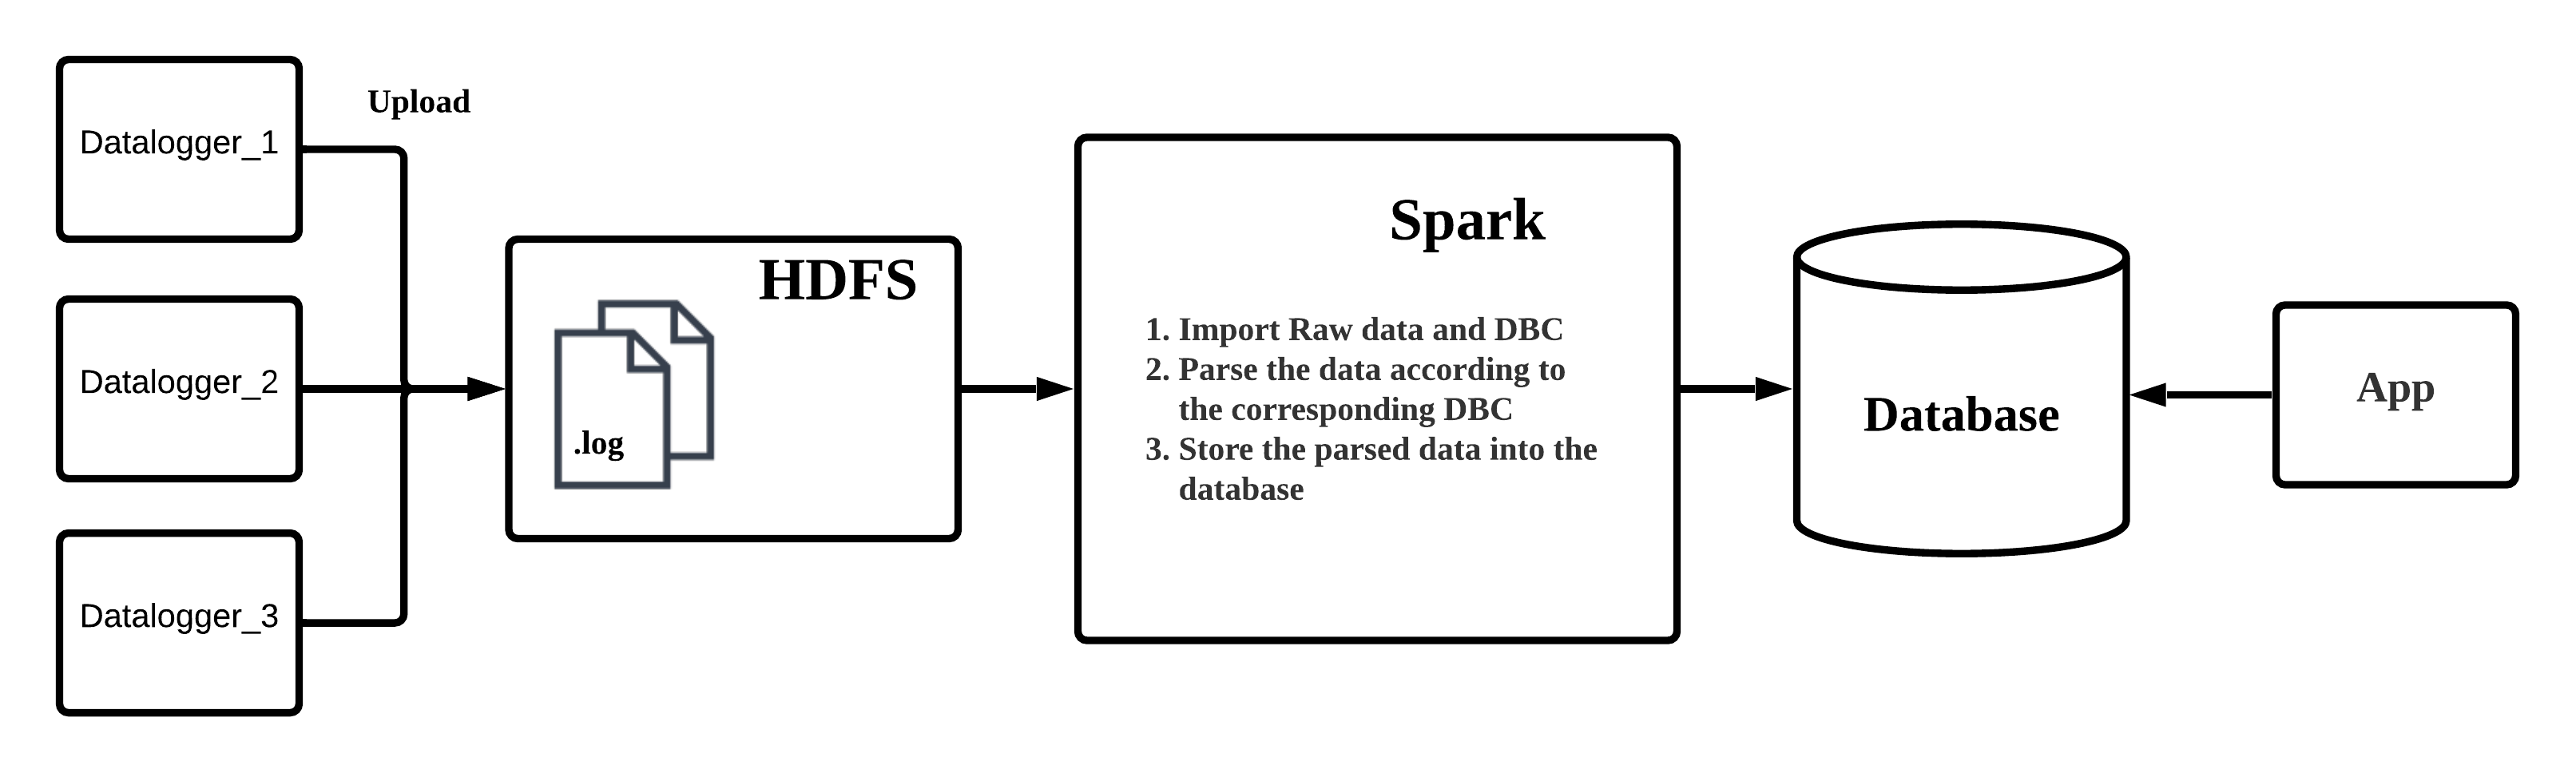
\includegraphics[width=0.9\textwidth]{gfx/process.png}
    \caption{System architecture diagram}
    \label{fig:system_architecture}
\end{figure}
As shown in the Figure \ref{fig:system_architecture}, The execution process can be divided into the following steps:
\begin{enumerate}
    \item Raw CAN-Trace comes from real cars or car test benches, collected by Datalogger.
    \item Upload each datalogger's CAN bus data to the Hadoop Distributed File System (HDFS).
    \item Parsing raw CAN bus data from HDFS with Spark based on DBC file.
    \item Writing of the parsed CAN bus data to the database.
    \item Users can download raw trace directly from Hadoop Distributed File System (HDFS) or use SQL-query to get data in the database
\end{enumerate}


\renewcommand{\lstlistingname}{Code} % Listing->Code
\begin{lstlisting}[caption=The entire process via Spark, style=myScalastyle, label=lst:mysql_cp]
  def executeModel() = {
    // a. Init Spark
    init()
    try {
      // b. Get DBC data
      val dbcDF = getDBC(AUDI_A8)
      dbcDF.persist(StorageLevel.MEMORY_AND_DISK)
      // c. Get Raw-Trace
      val traceDF = getTraceData()
      // d. Parse trace according to DBC
      val resultDF = parseTrace(dbcDF, traceDF)
      // e. Write result to database
      saveResult(resultDF)
    } catch {
      case e: Exception => e.printStackTrace()
    } finally {
      // f. close Spark
      close()
    }
  }
\end{lstlisting}




\section{Data flow of the implementation with Spark}
The data processing of CAN bus can be divided into the following main steps via Spark.
\begin{enumerate}
\item The raw CAN bus data are stored in binary form and uploaded to the HDFS file system of the server cluster. These binary files will be read by Spark and parsed later. Spark has a binary file data source that reads binary files and turns them into a single record including the file's raw content and metadata\cite{binary_file_data_spark}.

\renewcommand{\lstlistingname}{Code} % Listing->Code
\begin{lstlisting}[caption=Spark: Reading binary files, style=myScalastyle, label=lst:Reading binary files]
  def getRawTrace(path: String, spark: SparkSession): DataFrame = {
    val frame = spark.read
      .format("binaryFile")
      .load(path)
    frame
  }
\end{lstlisting}

% \begin{figure}[hbt!]
%     \centering
%     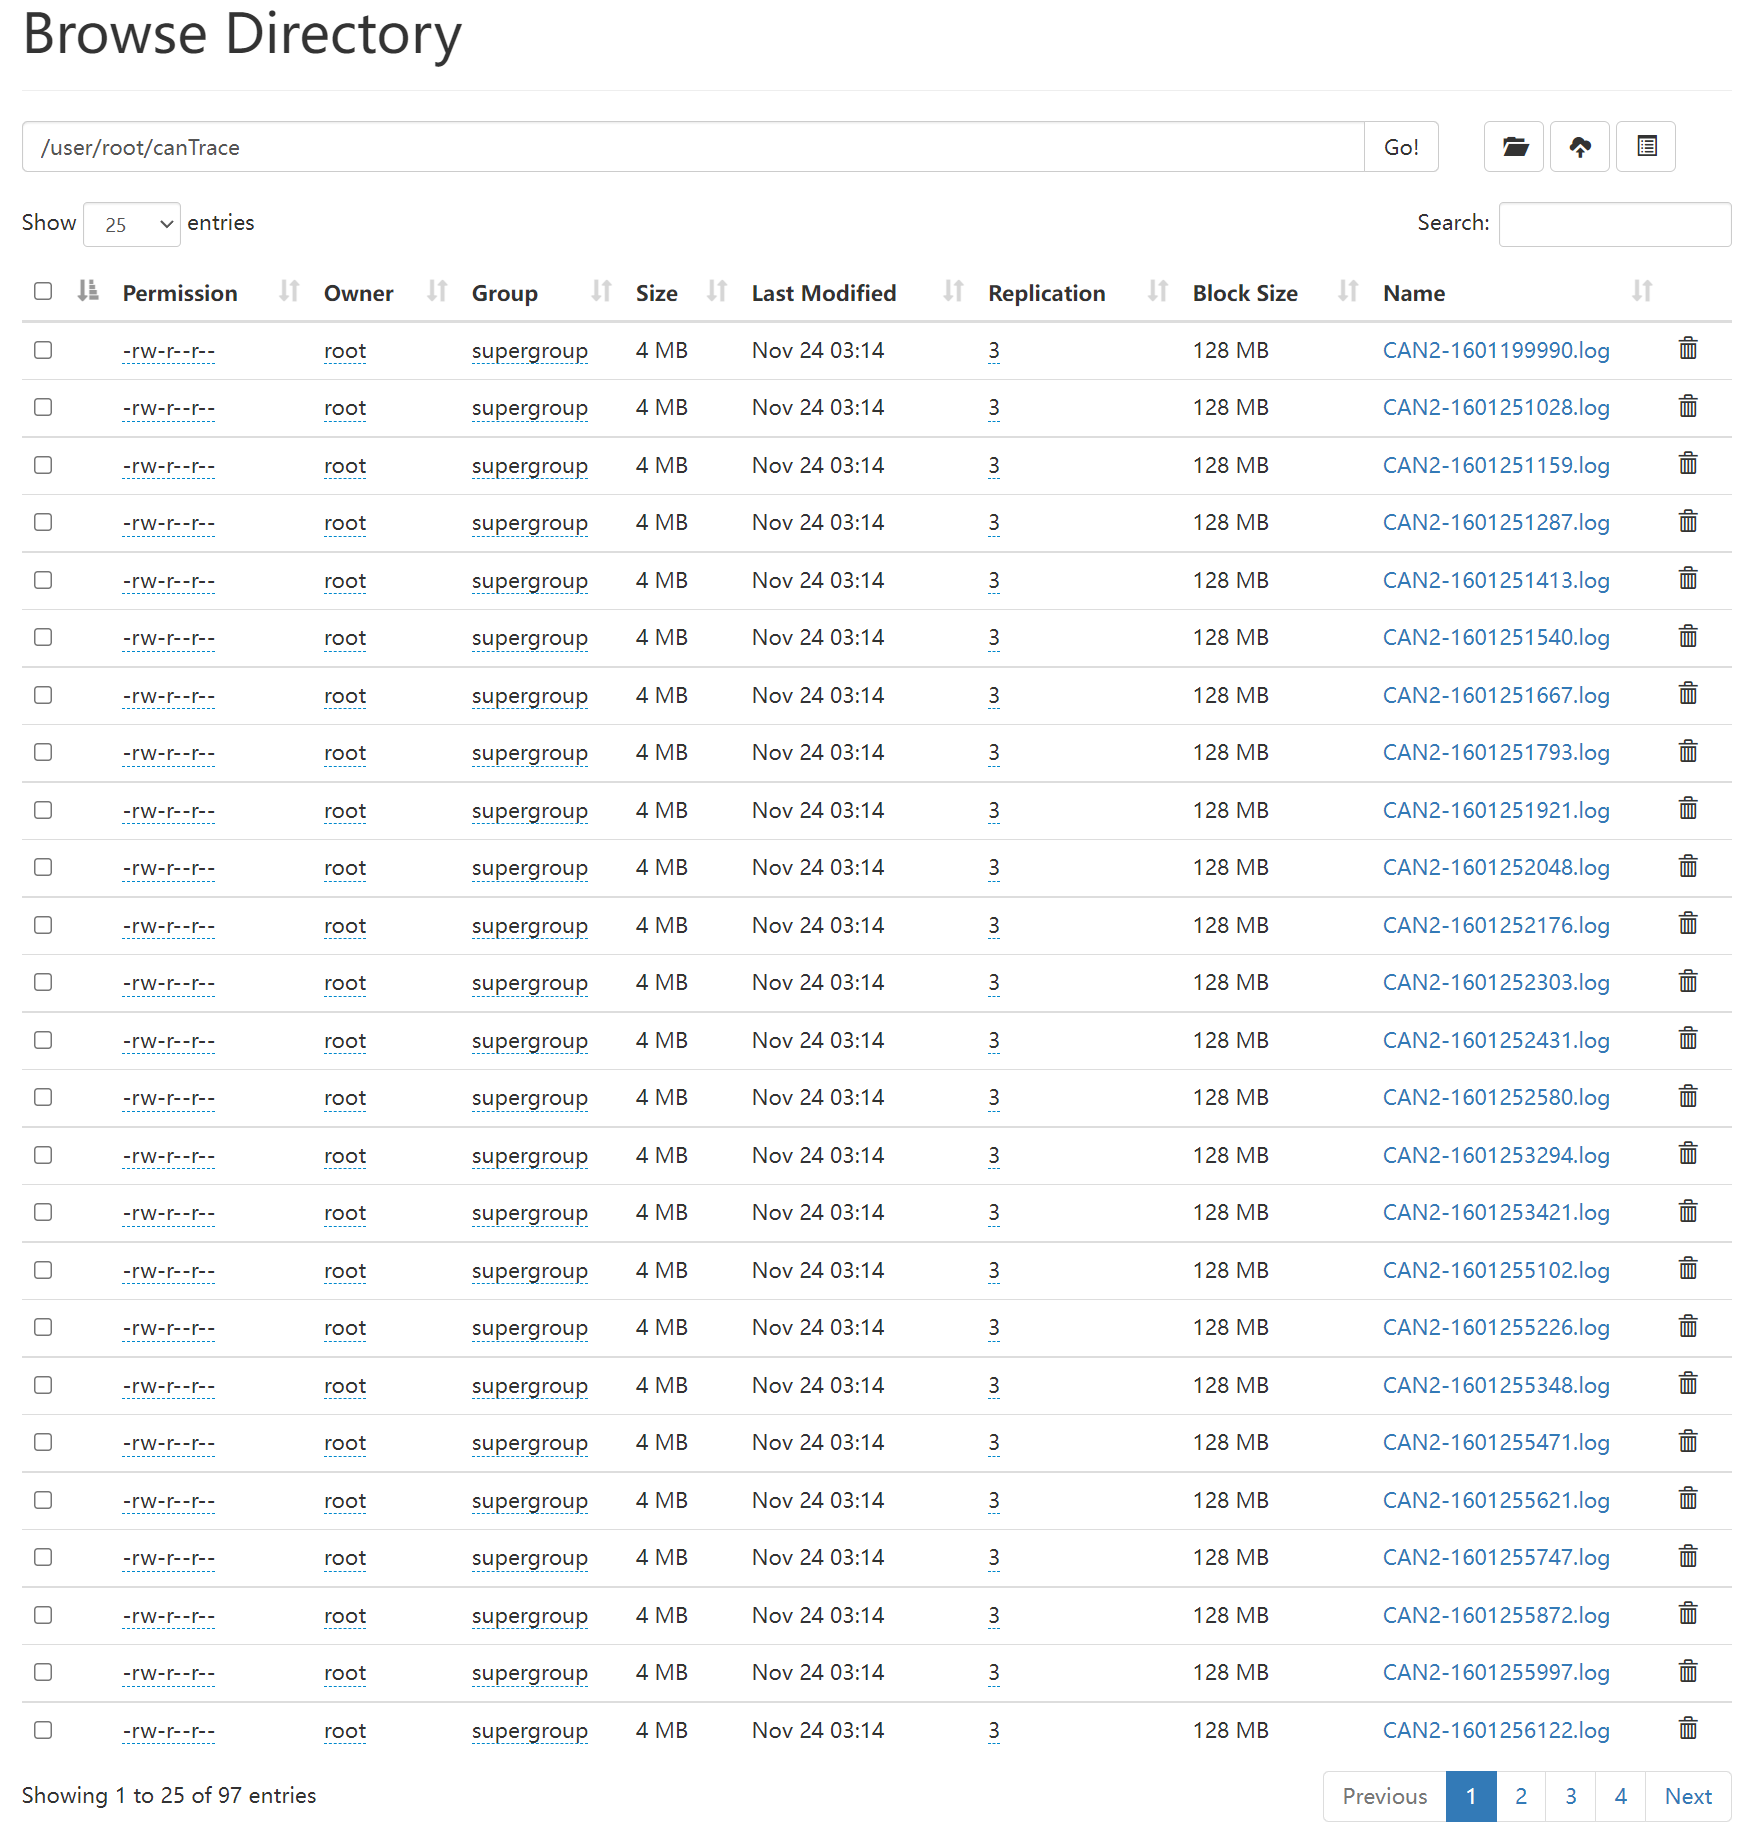
\includegraphics[width=0.5\textwidth]{gfx/hdfs.png}
%     \caption{Binary file of CAN-Trace in HDFS}
%     \label{fig:binary_can}
% \end{figure}

\begin{table}[hbt!]
\centering
\begin{tabular}{|l|l|l|l|}
\hline
\textbf{path}          & \textbf{modificationTime} & \textbf{length} & content                \\ \hline
file:/user/root/can... & 2021-09-28 05:15:56       & 4194331         & {[}5F 71 26 D0 03 7... \\ \hline
file:/user/root/can... & 2021-09-28 05:16:06       & 4194331         & {[}5F 71 37 35 05 0... \\ \hline
file:/user/root/can... & 2021-09-28 05:16:16       & 4194331         & {[}5F 71 43 A9 05 1... \\ \hline
file:/user/root/can... & 2021-09-28 05:16:18       & 4194331         & {[}5F 71 48 D0 04 4... \\ \hline
file:/user/root/can... & 2021-09-28 05:16:24       & 4194331         & {[}5F 71 50 63 02 5... \\ \hline
\end{tabular}%
\caption{Raw binary file data read by Spark}
\label{tab:raw_spark}
\end{table}

\item First clean the binary dataframe, remove the unnecessary data and convert it from binary to hexadecimal according to the CAN bus protocol.

\renewcommand{\lstlistingname}{Code} % Listing->Code
\begin{lstlisting}[caption=Spark: Converting to hexadecimal, style=myScalastyle, label=lst:Converting_hexadecimal]
  def getHexTrace(binaryFrame: DataFrame): DataFrame = {
    binaryFrame.flatMap(ele => {
      val DataBuffer_StartIdx = head_size
      val arrayByte = ele.get(3).asInstanceOf[Array[Byte]]
      var buffer = ByteBuffer.wrap(arrayByte)
      var canList = new ListBuffer[DataCAN_1]

      while (buffer.capacity() >= head_size) {
        val header = parseBufferFrameHeader(buffer)
        val length = header.length
        buffer.position(DataBuffer_StartIdx)
        buffer.limit(DataBuffer_StartIdx + length)
        val dataBuffer = buffer.slice()
        val dataTrace = parse(dataBuffer)
        val trace = convert2ASC(dataTrace, header)
        canList += trace
        buffer.position(DataBuffer_StartIdx + length)
        buffer.limit(buffer.capacity())
        buffer = buffer.slice()
      }
      canList
    }).orderBy("ts")
      .toDF()
  }
\end{lstlisting}

\begin{table}[hbt!]
\centering
\begin{tabular}{|l|l|l|}
\hline
Timestamp        & ID        & Data                    \\ \hline
1601199986095518 & 779       & 32 09 00 01 01 00 00 4E \\ \hline
1601199986099540 & 389226768 & 93 E3                   \\ \hline
1601199987003519 & 389232401 & 48 7A                   \\ \hline
1601199987007539 & 424       & B9 03 05 43 21 FF FF 7E \\ \hline
1601199987011518 & 201       & 00 1F 08 00 00 05 00 0F \\ \hline
\end{tabular}
\caption{Part of the Dataframe after parsing according to CAN bus protocol}
\label{tab:my-table}
\end{table}

\item According to DBC the Dataframe is parsed using \ac{udf} of Spark, which are one-row user-programmable procedures. The parsing process is shown in the following code.

\renewcommand{\lstlistingname}{Code} % Listing->Code
\begin{lstlisting}[caption=Spark: Parsing according to the DBC, style=myScalastyle, label=lst:parsing_algorithm]
  def parseHexCan(dbcDF: DataFrame, rawDF: DataFrame): DataFrame = {
    import dbcDF.sparkSession.implicits._
    val parseCAN_udf = udf {
      (canMsg: Array[Int], info: Seq[Row]) => {
        val details = new Array[Long](info.size)
        var num = 0
        info.zipWithIndex.foreach {
          case (row, i) => {
            var value: Long = 0
            val name = row.getAs[String](0)
            val len = row.getAs[Int](2)
            var start = row.getAs[Int](1) % 8
            var bitLen = len
            var position = Math.ceil(row.getAs[Int](1) / 8).toInt
            while (bitLen > 0) {
              if (start + bitLen <= 8) {
                val mask = (Math.pow(2, bitLen) - 1).toLong
                value += ((canMsg(position) >> start) & mask) << (len - bitLen)
                start += bitLen
                bitLen = 0
              } else {
                value += (canMsg(position) >> start) << (len - bitLen)
                bitLen -= 8 - start
                start = 8
              }
              if (start == 8) {
                position += 1
                start = 0
              }
            }
            details(i) = value
          }
        }
        details
      }
    }
    rawDF
      .join(dbcDF, rawDF("id") === dbcDF("identifier"), "inner")
      .select($"module", rawDF("ts"), rawDF("id"), $"data", dbcDF("info"))
      .orderBy("id", "ts")
      .withColumn("map", parseCAN_udf('data, 'info))
      .drop("info", "data")
  }
\end{lstlisting}

\begin{table}[hbt!]
\centering
\resizebox{\textwidth}{!}{%
\begin{tabular}{|l|l|l|}
\hline
\textbf{Timestamp} & \textbf{ID} & \textbf{Data}                            \\ \hline
1601199986095518 & 779 & {[}0, 0, 0, 0, 1, 0, 0, 0, 5, 0, 0, 0, 0, 0, 0, 0, 0, 0, 0, 0, 1, 0, 0, 0, 0, 0, 0, 0, 0, 0{]} \\ \hline
1601199986099540   & 389226768   & {[}144{]}                                \\ \hline
1601199987003519   & 389232401   & {[}128{]}                                \\ \hline
1601199987007539   & 424         & {[}101, 11, 4096, 4096, 4096, 0, 0, 0{]} \\ \hline
1601199987011518 & 201 & {[}0, 31, 0, 0, 0, 0, 0, 0, 0, 0, 0, 0, 0, 0, 0, 0, 0, 254, 0, 0, 0, 0, 3{]}                   \\ \hline
\end{tabular}%
}
\caption{Part of the Dataframe after parsing according to DBC}
\label{tab:after_parsing}
\end{table}

\item The parsed data will be written to different tables in the database based on the CAN ID.

\end{enumerate}

\section{Definition of database table structure}

\begin{figure}[hbt!]
	\centering
 	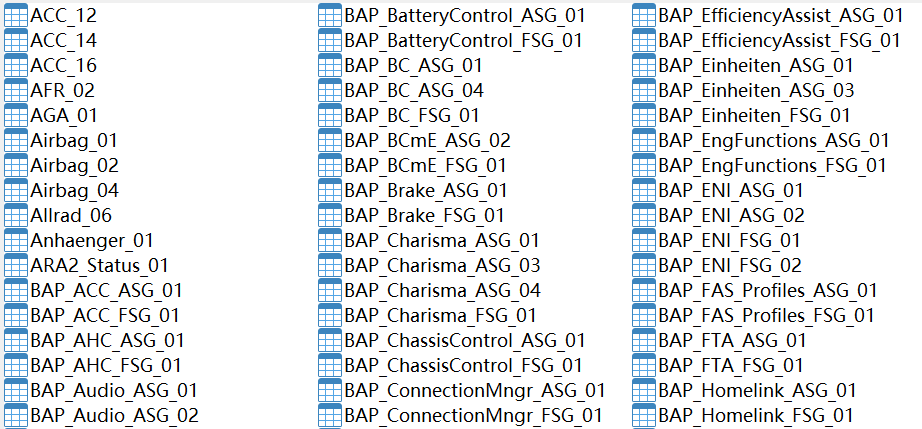
\includegraphics[width=0.6\textwidth]{gfx/tables.png}  	  	 	
	\caption{Tables of CAN-ID}
	\label{fig:tables_can}
\end{figure}

The choice of database is also the focus of the next chapter and this subsection only describes how the tables are created for each database. From the DBC file, the corresponding tables are created in each database and each table is associated with a CAN ID. Take for example the DBC for audi\_a8, a database with a total of 520 tables. The Figure \ref{fig:tables_can} below shows some of the tables in the database. The exception is InfluxDB, which does not create tables (Measurements) in advance, as it is a schemaless database. 

As the parsed data is structured data, the most appropriate data type is selected for each column based on the DBC file when creating the table in order to be able to store the data in the database small enough. Take CAN ID Motor\_12 for example, the parsed data with a value of 0-255 is of type TINYINT UNSIGNED in MySQL. It should be noted that different databases have different names for their data types, for example TINYINT UNSIGNED in MySQL, and UINT8 in ClickHouse. 

\begin{figure}[htb]
	\centering	
	\subcaptionbox{DBC rule of Motor12 %
		\label{fig:example_2}}%
 		[.48\linewidth]{
  		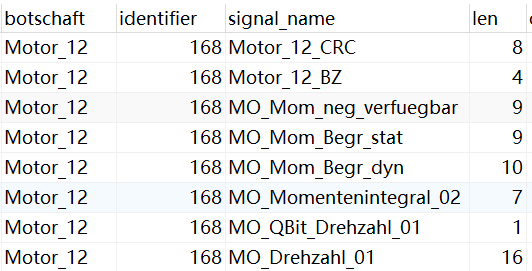
\includegraphics[width=0.35\textwidth]{gfx/motor_12_mysql.png} 	
  	}  	
  	~
  	\subcaptionbox{Data type of Motor12 in MySQL %
  		\label{fig:example_3}}
 		[.48\linewidth]{
  		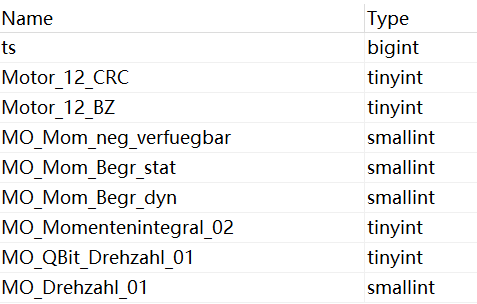
\includegraphics[width=0.35\textwidth]{gfx/datatype_mysql.png}  	
  	}	  
  		
	\caption{}
	\label{fig:ex_2_3}
\end{figure}


%*****************************************
\chapter{Choice of Databases}
\label{ch:choice_of_databases}
By writing CAN bus information into the database, users can query the required data according to their needs. There are different types of databases, such as Relational databases, NoSQL databases, Columnar databases, Wide column databases, Key-value databases, Document databases, and so on. What kind of database is suitable for storing and querying large amount of CAN bus data, this chapter will introduce several databases that will be tested later. However, before introducing various databases, it is important to first introduce the basic structure of data storage and indexing, because different structures play a big role in database read and write performance. In representative relational databases such as MySQL, the basic structure of data storage and indexing is the widely used B+ tree. And in some mainstream NoSQL databases such as HBase and Cassandra, the log structure merge (LSM) tree is used. 

A total of four databases are selected, which represent different types of databases. MySQL is a relational database using B+ tree structure, the rest using LSM-tree structure are ClickHouse which is a column-oriented database specifically for OLTP, Cassandra which is a wide column storage database, and InfluxDB which is a time-series database.

\section{Data structure for Disks}
\label{lsm_bplus}

For the performance of a database, the way in which its data is structured is crucial. Most of the data in a database is stored on disk, and disk I/O is a very time-consuming operation compared to memory I/O. Therefore, one of the key points to improve the speed of database data queries is to minimise the number of disk I/O\cite[p.~2]{10.1007/s002360050048}. The current underlying data structure of the database is divided into two main structures, B+ tree or LSM tree, and each has its own set of pros and cons. For the database tested later (Chapter \ref{ch:database_performancecomparison}), MySQL used B+ tree, while the rest of the databases used LSM-Tree.

\subsection{B+ Tree}
\begin{enumerate}
\item Overview
    
B+ tree is a tree data structure, usually used in databases and operating system file systems. B+ Tree is a B-Tree extension that allows for faster insertion, deletion, and search operations. In contrast to the B-Tree, records (data) can only be stored on leaf nodes in a B+ tree, while key values can only be stored on internal nodes\cite{b_plus}.



\item Rules of B+ Tree

\begin{itemize}
    \item There are at least two children in the root.
    \item Data records are stored on leaves.
    \item If the target key value is less than the internal node, the point directly to the left is followed. If a target key value is larger than or equal to the internal node, the point immediately to its right is used\cite{walker_2021}.
    \item The height of the leaf nodes is the same.
    \item Internal nodes are used as indexes.
\end{itemize}

\begin{figure}[hbt!]
	\centering
 	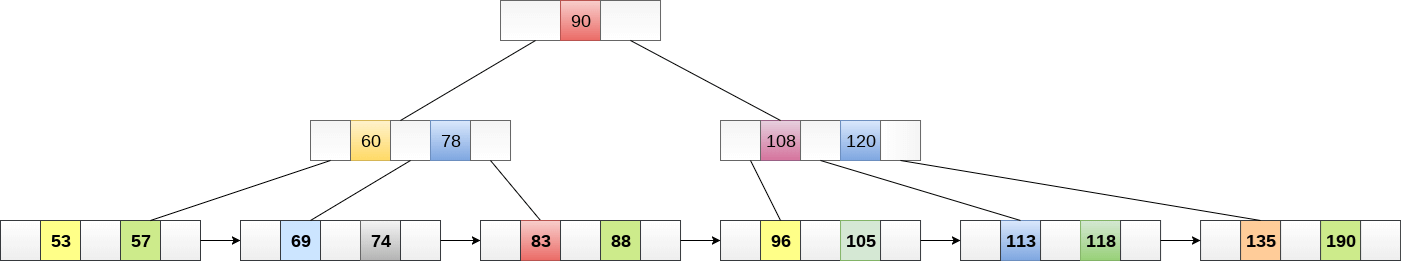
\includegraphics[width=0.7\textwidth]{gfx/b-plus-tree.png}
	\caption{Structure of B+ tree \cite{johnny_2016}}
	\label{fig:bplus_structure}
\end{figure}

\item Features of B+ trees

\begin{enumerate}
    \item All keywords appear in a chained table of leaf nodes (dense index) and the keywords in the chained table happen to be ordered.
    \item It is impossible to find at internal nodes.
    \item It is better suited for file indexing systems.
    \item Leaf nodes are equivalent to data layers for storing (keyword) data, and internal nodes are equivalent to indexes of leaf nodes (sparse indexes).
\end{enumerate}



\item Writing process of B+ tree
\begin{enumerate}[label=\arabic*)]
    \item Find the leaf node L to be inserted\cite{johnny_2016}.
    \item Then insert the data item into this node L. If no node is in violation, the process ends. If there is a violation, a splitting operation is performed. Otherwise, split leaf node L evenly into two nodes (L and the new node L2)\cite{walker_2021}.
    \item Continue this process recursively up the tree until the root node is reached.
    \item A new root node is generated if the root node is split.
\end{enumerate}


\item Search process of B+ tree

Starting at the root node, the index entries of the internal nodes are checked and a binary search can be used to find the corresponding child node. The related record is returned to the user if the search key is an exact match\cite{walker_2021}.

\item Delete process of B+ tree

\begin{enumerate}[label=\arabic*)]
    \item Starting at the root node, find the leaf node to which the item belongs.
    \item Delete this item. The operation is done if the leaf node only fulfills the satisfactory criteria of being half full. The Leaf node, on the other hand, has only a few elements and cannot be erased\cite{walker_2021}.
    \item If a merge occurs, the index item must be removed from the parent node of leaf node.
    \item Recurse this process until the node is legal, or until the root node is reached\cite{walker_2021}.
\end{enumerate}


\item Uses of B+ trees

B+ trees are mainly suitable for indexing operations, and here there are two main reasons. 

\begin{itemize}
    \item The query efficiency of B+ trees is more stable.  Since the internal node is not the node that ultimately points to the contents of the file, but only an index of keywords in the leaf nodes. So any keyword query must take a path from the root node to a leaf node. All keyword queries have the same path length, resulting in comparable query efficiency for each piece of data.
    \item B+ trees have lower disk I/O consumption. The internal nodes of the B+ tree do not have pointers to keyword-specific data. If all keywords from the same internal node are stored in the same disk block, the more keywords the disk block can hold. This means that the more keywords are read into memory at one time and the number of IO is also reduced.
\end{itemize}

\end{enumerate}
\subsection{LSM-Tree}

\begin{enumerate}
\item Overview

\ac{lsm} is based on the assumption that memory is large enough that data does not need to be written to disk each time it is updated. Instead, the data is stored in memory, where it is merged and appended to the end of the disk using subsumption sorting after a given amount of accumulation. The LSM-Tree can be quickly merged to disk by merging and sorting because it is ordered\cite{lsm_tree}. By transforming random disk writes to disk sequential writes, LSM-Trees significantly increase write throughput.

\item LSM-Tree Storage Model

\begin{figure}[hbt!]
	\centering
 	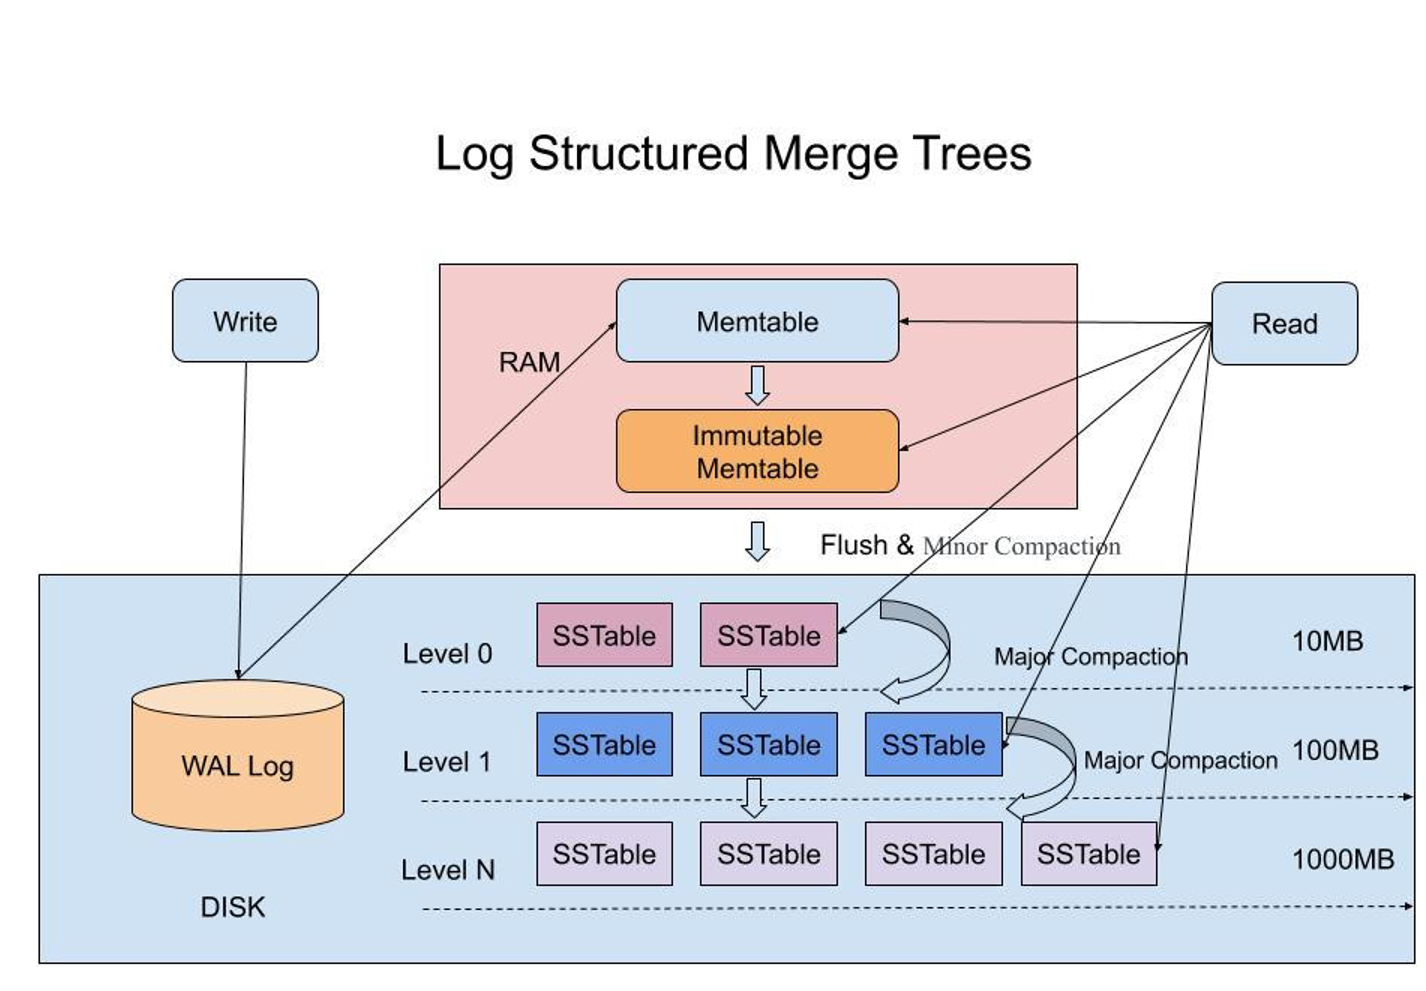
\includegraphics[width=0.7\textwidth]{gfx/structure_lsm.png}
	\caption{Structure of LSM-Tree}
	\label{fig:lsm_structure}
\end{figure}

\begin{itemize}
    \item \ac{wal}
    
    When a row of data is inserted, it is first written sequentially to the WAL file and then inserted into the MemTable in memory\cite{lsm_tree}. The MemTable in memory can be recovered from the WAL file once the server is turned down.
    
    \item MemTable
    
    MemTable is the memory storage structure for WAL files, usually implemented as a SkipList, and provides an interface for writing, deleting and reading k-v data. MemTable internally stores key-value pairs in an ordered manner according to key values, so that they can be quickly serialised to an SSTable file and saved to an SSTable file, still preserving the orderliness of the data\cite{lsm_tree}.
    
    \item Immutable MemTable
    
    Immutable MemTable is a read-only MemTable in memory. As memory is limited, normally a threshold is set and when this threshold is exceeded, the data in the MemTable is converted into an Immutable MemTable and then the system generates a new MemTable for reading and writing to continue. The essence of using Immutable Memtable is to avoid blocking write operations when serialising the data in the MemTable to disk\cite{lsm_tree}. 
    
    \item \ac{sstable}
    
    SSTable is an ordered storage of data on disk in a MemTable, where the internal data is ordered according to key. Often to speed up queries, it is necessary to add data indexes to the SSTable so that the specified key-value pair data can be located quickly. When the data in MemTable reaches a specified threshold, a new SSTable is created at Level 0. When the number of files under a Level exceeds a certain number, one of the SSTable files under that Level is merged with a higher level SSTable file\cite{lsm_tree}. The process is shown in the Figure \ref{fig:sstable}.
    
    \begin{figure}[hbt!]
	\centering
 	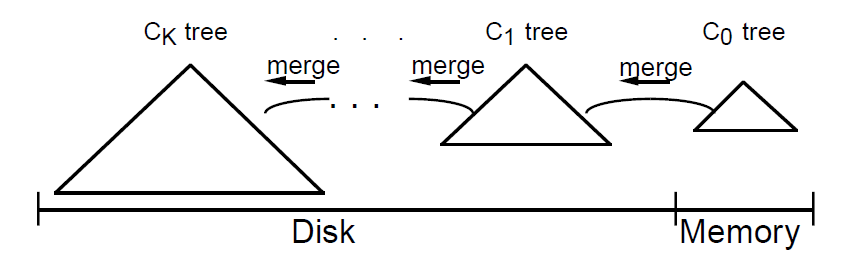
\includegraphics[width=0.5\textwidth]{gfx/sstable.png}
	\caption{An LSM-tree of K+1 components \cite[p.~15]{10.1007/s002360050048}}
	\label{fig:sstable}
\end{figure}

\end{itemize}

\item Writing process of LSM-Tree

\begin{enumerate}[label=\arabic*)]
\item The operation is written to the WAL file and used for fault recovery when a write request is received.
\item After the WAL is written, the data is written to MemTable in-memory.
\item When the MemTable exceeds a certain size, it is frozen in memory and becomes an immutable MemTable, while a new MemTable is created to continue the service without blocking writes.
\item Writing the immutable MemTable in memory to the SSTable layer on the hard disk is also known as Minor Compaction.
\item Once the SSTable on each tier of the disk reaches a specific size or number, it will be merged on a constant schedule. This step is also known as Major Compaction.
\end{enumerate}

\item Reading process of LSM-Tree

LSM-Tree when needing to read data based on Key, first look in the MemTable and Immutable MemTable in memory, if not found, continue from Level 0, if not found, continue to look in the SSTable file from higher levels\cite{lsm_tree}. If the search fails, the data does not exist in the entire LSM-Tree.

\end{enumerate}

\subsection{B+ Tree vs LSM Tree}

Three key criteria for evaluating a data structure's performance are write amplification, read amplification, and space amplification\cite{tikv}.

\begin{enumerate}
    \item Write Amplification: The ratio of data written to the storage device against data written to the database
    
    \item Read Amplification: The number of disk reads per query. Read amplification is defined separately for point query and range queries. For range queries the range length matters (the number of rows to be fetched)\cite{tikv}.
    
    \item Space Amplification: The ratio of the amount of data on the storage device versus the amount of data in the database\cite{tikv}.
\end{enumerate}

\paragraph{B+ tree}
To make the analysis easier, assume that the tree's block size is $B$ bytes, and that keys, pointers, and records are of the same size, so that each internal node has $O(B)$ children and each leaf has $O(B)$ data records. Then the depth of the tree is $O(log_B N/B)$ where $N$ is the size of the database\cite{tikv}.

\begin{itemize}
    \item Write Amplification
    
    Because every insertion in the worst-case conditions necessitates writing the leaf block containing the record, the write amplification is $B$.
    
    \item Read Amplification
    
    The number of disk reads per query is at most $O(log_B N/B)$, which is the depth of the tree.
\end{itemize}

\paragraph{LSM-Tree}
Data is structured into levels in the Level-based LSM-tree, and each level comprises one sorted run. The sizes of each level are limited. The magnification of data size at each level is defined by the growth factor $k$. The number of levels is $O(log_k N/B)$ where $N$ is the size of the database if the growth factor is $k$ and the smallest level is a single file of size $B$\cite{tikv}.

\begin{itemize}
    \item Write Amplification
    
    Each level's data must be transported out just once, although data from one level is constantly blended with data from the previous level\cite{tikv}. Each data item is remerged into the same level around $k/2$ times after being written into it the first time. As a result, the write amplification of LSM-Tree is $O(k*log_k N/B)$.
    
    \item Read Amplification
    
    For the highest $level_i$, the data size is $O(N)$, so that it performs $O(logN/B)$ disk reads.
    
    For the previous $level_i-1$, the data size is $O(N/k)$, so that it performs $O(log(N/(kB)))$ disk reads.
    
    ...
    
    For $level_i-n$, the data size is $O(N/k^n)$, so that it performs $O(log(N/(k^n B)))$ disk reads.
    
    The number of disk reads per query is
    $$O(logN/B) + O(log(N/(kB))) + O(log(N/(k^2 B))) + ... + O(log(N/(k^n B))) = O((log^2 N/B)/logk)$$
\end{itemize}

\paragraph{Summary}

\begin{table}[hbt!]
\centering
\begin{tabular}{@{}lll@{}}
\toprule
\textbf{Data Structure} & \textbf{Write Amplification} & \textbf{Read Amplification} \\ \midrule
B+ tree                 & $O(B)$                       & $O(log_B N/B)$              \\
LSM-Tree                & $O(k*log_k N/B)$             & $O((log^2 N/B)/logk)$       \\ \bottomrule
\end{tabular}
\caption{Amplification of B+ tree and LSM-Tree \cite{tikv}}
\label{tab:amplification}
\end{table}

From the Table \ref{tab:amplification}, we conclude that LSM-tree outperforms B+ tree in terms of write performance, but not in terms of read performance.

When writing data to B+ tree, WALs and pages are written and the whole page is written each time. Page splitting may also occur. LSM-Tree writes are not page-oriented operations and take better advantage of sequential writes, which are generally faster.

B+ tree tends to have a greater advantage for precise query requirements. Not only that, but in scenarios where transactions need to be implemented, it is also easier for the database to use B+ tree because locks can be implemented directly on the tree. The LSM-Tree structure, on the other hand, may have to add other data structures in order to implement locks.

\section{Row and Column oriented storage}
\label{row_column_storage}

\subsection{Row oriented}
The properties of a certain record are added first in a Row Oriented Database, and then the following record is inserted. The data is saved row by row in a row-oriented database, with the start column of each row being next to the final column of the preceding row. As a result, when multiple columns of a single row must be selected at the same time, row-oriented systems are more productive\cite{6495251}. 

\begin{table}[hbt!]
\centering
\begin{tabular}{@{}|l|lll|@{}}
\toprule
RowID & \multicolumn{1}{l|}{Col1} & \multicolumn{1}{l|}{Col2} & Col3 \\ \midrule
1     & \multicolumn{3}{l|}{--------------------$\longrightarrow$}                       \\ \midrule
2     & \multicolumn{3}{l|}{--------------------$\longrightarrow$}                       \\ \midrule
3     & \multicolumn{3}{l|}{--------------------$\longrightarrow$}                       \\ \bottomrule
\end{tabular}
\caption{Data storage pattern in Row Oriented Database}
\label{tab:row_oriented}
\end{table}

\paragraph{Reading from Row Store Storage}
When fetching a row or a collection of rows, row oriented databases are fast, but when conducting an aggregation, they bring extra data (columns) into memory, which is slower than merely selecting the columns you want to aggregate on\cite{6495251}. Furthermore, the number of disks that a row-oriented database may need to access is typically greater.

\paragraph{Writing to Row Store Storage}
If there is a new row of data that needs to be added to the database, it can be appended to the end of the current data. Row-oriented databases are still commonly used in online transaction processing (OLTP) style applications because they can manage writes to the database very well\cite{6495251}.

\subsection{Column oriented}

\begin{table}[hbt!]
\centering
\begin{tabular}{|l|c|c|c|}
\hline
RowID & Col1         & Col2         & Col3         \\ \hline
1     & |            & |            & |            \\ \cline{1-1}
2     & |            & |            & |            \\ \cline{1-1}
3     & $\downarrow$ & $\downarrow$ & $\downarrow$ \\ \hline
\end{tabular}
\caption{Data storage pattern in Column Oriented Database}
\label{tab:column-oriented}
\end{table}

The column-oriented storage stores the different columns of a record in different files, whereas the row-oriented storage stores the data of the same record row by row in a file. After storing the columns in different files, the column database usually also compresses the columns, because the data in the same column is relatively similar and has the possibility to be compressed\cite[p.~96]{kleppmann2017designing}. 


\begin{table}[hbt!]
\centering
\begin{tabular}{|c|c|c|c|}
\hline
\textbf{Timestamp} & \textbf{Motor\_12\_CRC} & \textbf{Motor\_12\_BZ} & \textbf{MO\_Mom\_neg\_verfuegbar} \\ \hline
1601199986096455 & 144 & 15 & 510 \\ \hline
1601199986097467 & 248 & 0  & 510 \\ \hline
1601199986098479 & 130 & 1  & 510 \\ \hline
\end{tabular}%
\caption{Row-oriented storage of CAN bus data in Motor\_12}
\label{tab:row_oriented}
\end{table}


\begin{table}[hbt!]
\centering
\resizebox{\textwidth}{!}{%
\begin{tabular}{ll}
Columnar storage layout                 &                                                      \\
Timestamp file contents:                & 1601199986096455, 1601199986097467, 1601199986098479 \\
Motor\_12\_CRC file contents:           & 144, 248, 130                                        \\
Motor\_12\_BZ file contents:            & 15, 0, 1                                             \\
MO\_Mom\_neg\_verfuegbar file contents: & 510, 510, 510                                       
\end{tabular}%
}
\end{table}

~\\
\paragraph{Column Compression}
A higher compression ratio can be achieved with columnar storage than with row storage, further reducing the need for disk throughput\cite[p.~97]{kleppmann2017designing}. As shown in the above table for Motor\_12, the same column has the same type of data and a high degree of repetition. Therefore, different compression algorithms can be used for various columns.

The following compression algorithms are often used in time-series data.

\begin{itemize}
    \item Delta encoding
    
    The timestamp is usually stored in the long type and takes up 8 byte of storage space. By storing only the difference (or delta) between a data object and one or more reference objects, delta-encoding (also known as Delta compression) decreases the amount of information necessary to represent a data object. In storing time-series data, it is possible to save disk usage by storing only the previous time increment\cite{lockerman_2022}. 
    
    $$ Delta = T_n - T_{n-1} $$
    The following Table shows CAN bus time series data as an example.
    
    \begin{table}
            \footnotesize
                \begin{tabular}[t]{|p{3.2cm}|c|}
                    \hline
                    Timestamp\\ \hline
                    1601199986096455 \\ \hline
                    1601199986097467\\ \hline
                    1601199986098479 \\ \hline   
                \end{tabular}
                \hfill
                \begin{tabular}[t]{|p{3.2cm}|c|}
                    \hline
                    Timestamp\\ \hline
                    1601199986096455 \\ \hline
                    1012\\ \hline
                    1012 \\ \hline   
                \end{tabular}
                \hfill
                \begin{tabular}[t]{|p{3.2cm}|c|}
                    \hline
                    Timestamp\\ \hline
                    1601199986096455 \\ \hline
                    1012\\ \hline
                    0 \\ \hline   
                \end{tabular}
                \caption{Raw timestamp data \& Delta encoding data \& Delta-of-delta encoding data}
                \label{delta_delta}
            \end{table}
    
    
    \item Delta-of-delta encoding
    
    It applies the delta encoding again to the delta encoded data\cite{}. For time series data sets where data is collected regularly, we can apply delta-of-delta encoding to the time columns and actually only store a series of zeros\cite{lockerman_2022}. The delta-of-delta algorithm further achieves a higher compression ratio than the delta algorithm. In a practical scenario, the timestamps of a large amount of time-series data are dense and continuous, and most of them satisfy the $ delta-of-delta=0 $ condition, which can significantly reduce the storage space for timestamps\cite{10.14778/2824032.2824078}.
    
\end{itemize}

Not only can time series data be compressed, but other columns can also be compressed, e.g. Run-length encoding algorithms are often used for data with a large number of repetitions.

\begin{itemize}
    \item \ac{rle}
    
    \ac{rle} is a form of lossless data compression in which runs of data (sequences in which the same data value occurs in many consecutive data elements) are stored as a single data value and count, rather than as the original run\cite{wikipedia_rle}.
    
    As an example, the data of MO\_Mom\_neg\_verfuegbar can be used because it has a lot of repetitive data (Table \ref{tab:mom_rle}). The data in the column is stored in this form:
    
    510, 510, 510, 510, 535, 535
    
    We don't need to save each instance of the value. Instead, the number of repetitions is stored. This set of numbers could be stored as \{run; value\} pairs \cite{lockerman_2022} like this:
    
    \{510:4\}, \{535:2\}
    
    Compared to the previous uncompressed form, the disk storage is drastically reduced. The CAN bus data has a lot of repetitive data, which can be reduced by the RLE compression algorithm.
    
\begin{table}[hbt!]
\centering
\begin{tabular}{|c|}
\hline
MO\_Mom\_neg\_verfuegbar \\ \hline
510                      \\ \hline
510                      \\ \hline
510                      \\ \hline
510                      \\ \hline
535                      \\ \hline
535                      \\ \hline
\end{tabular}
\caption{Column of MO\_Mom\_neg\_verfuegbar}
\label{tab:mom_rle}
\end{table}
    
    
\end{itemize}
Many compression algorithms can be used together to achieve higher compression ratios, such as the previously mentioned Delta-of-Delta and RLE, or Delta-of-Delta and Simple8b(one of the simplest and smallest methods of storing variable length integers).


\paragraph{Vectorized processing}
Traditional OLTP databases usually use per-row calculations, the reason being that transactions are dominated by single point queries in transactions. SQL calculations are small and the benefits of vectorized processing are not obvious enough. 

Columnar storage databases use \ac{simd} instructions once for a batch of columnar data in memory (rather than once per row), which not only reduces the number of function calls and cache misses, but also allows the parallelism of SIMD instructions to be fully exploited, dramatically reducing computation time. Processor can run such a loop significantly faster than code that uses a lot of function calls and conditions for each row\cite[p.~99]{kleppmann2017designing}. The vectorized processing engine, in general, can deliver several times the performance improvement. 

In previous tests, ClickHouse used vectorized processing engine, so this is one of the reasons why it is so much faster than other databases in queries.

\paragraph{Writing to Column-Oriented Storage}

As mentioned in the previous section about the LSM tree writing process, all writes to a columnar store first go to an in-memory store (MemTable) where they are added to a sorted structure and prepared for writing to disk (MemTable). When the writes accrue to a certain level, they are combined with the column files on disk and written in bulk to new files, regardless of whether the in-memory store is row or column oriented\cite[p.~101]{kleppmann2017designing}.


\paragraph{Column families}
A column family is a database entity that has linked data columns in its columns. It's a tuple (pair) made up of a key–value pair, with the key mapped to a collection of columns as the value. A tuple (triplet) consists of a column name, a value, and a timestamp for each column\cite{wiki:Column_family}.

As Kleppmann \cite[p.~99]{kleppmann2017designing} stated, \enquote{Cassandra and HBase have a concept of column families, which they inherited from Bigtable. However, it is very misleading to call them column-oriented: within each column family, they store all columns from a row together, along with a row key, and they do not use column compression. Thus, the Bigtable model is still mostly row-oriented.}


\section{MySQL}
\begin{figure}[htb]
	\centering	
	\subcaptionbox{ %
		\label{fig:example_2}}%
 		[.49\linewidth]{
  		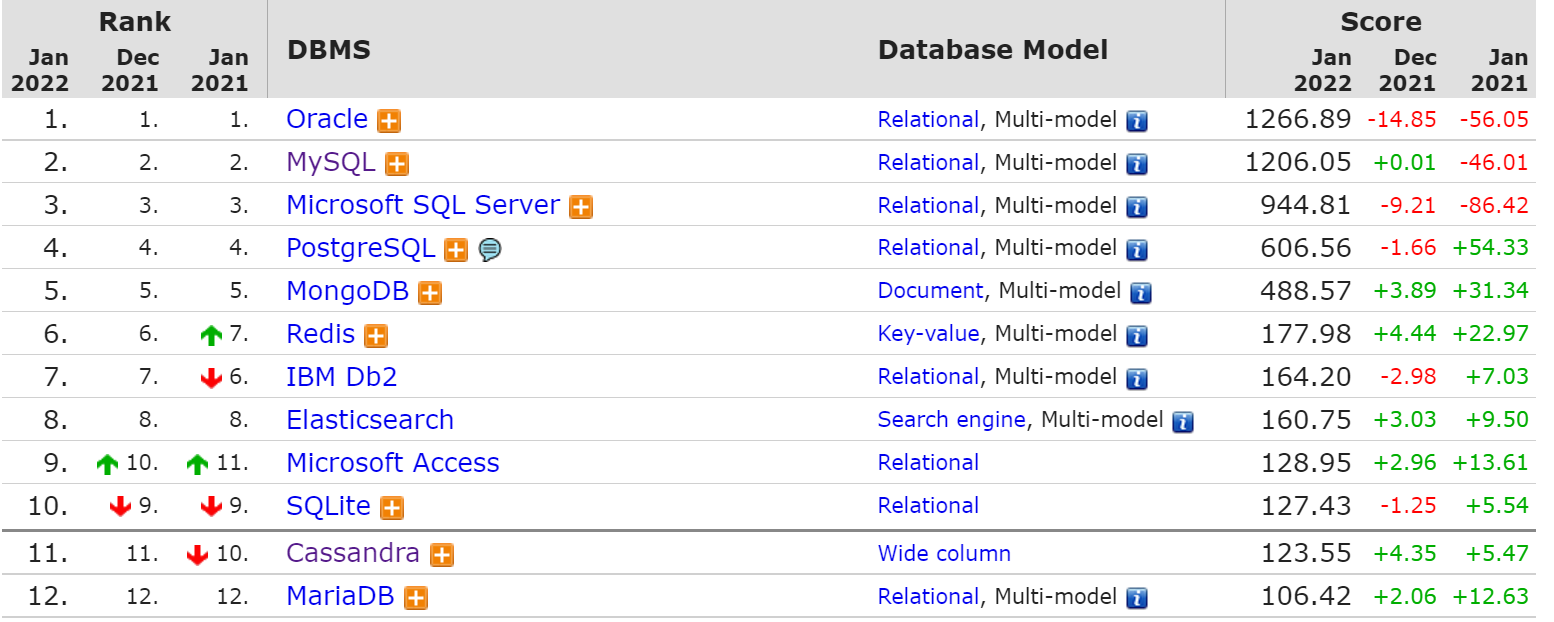
\includegraphics[width=0.35\textwidth]{gfx/database_ranking.png} 	
  	}  	
  	~
  	\subcaptionbox{ %
  		\label{fig:example_3}}
 		[.49\linewidth]{
  		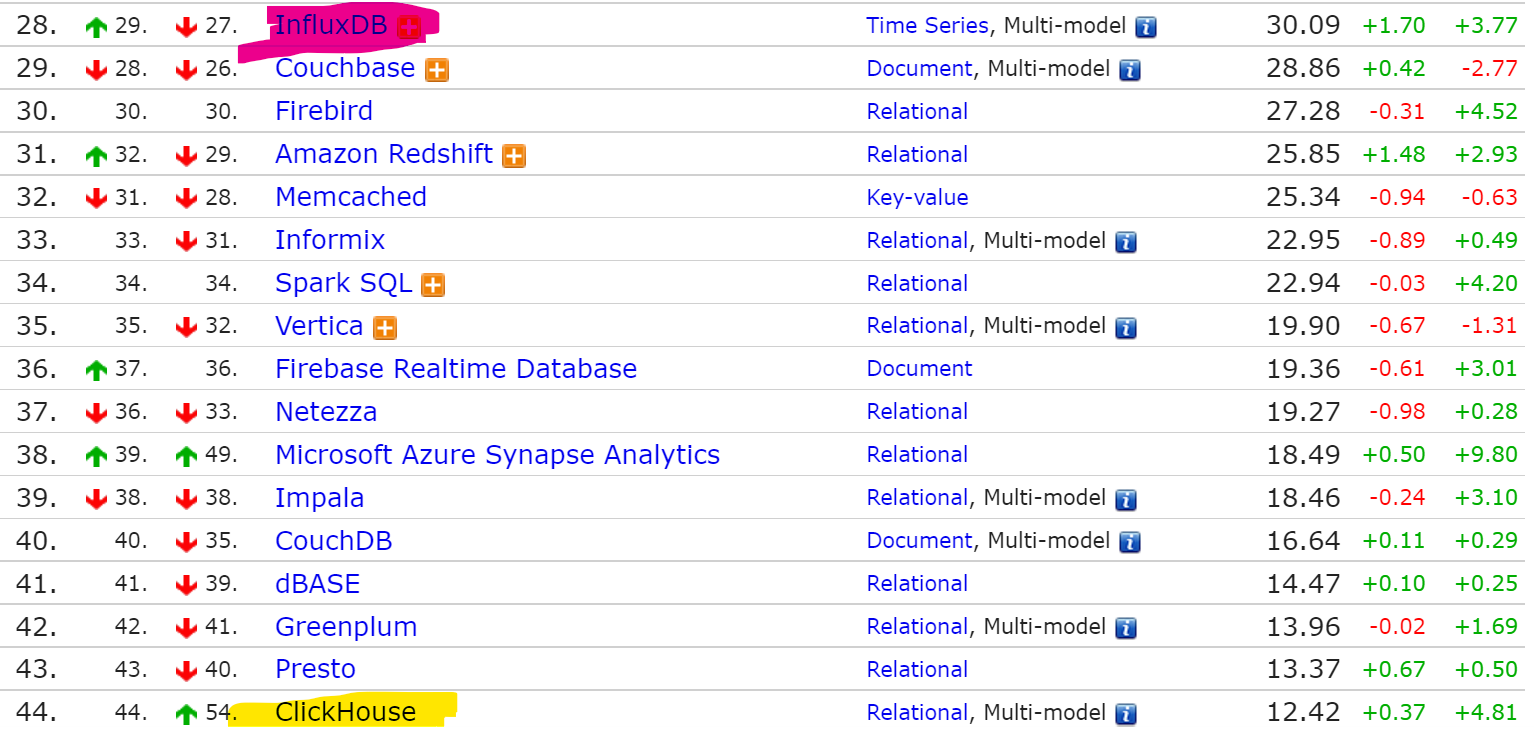
\includegraphics[width=0.35\textwidth]{gfx/database_ranking2.png}  	
  	}	  
  		
	\caption{Database-Engines Ranking\cite{db}}
	\label{fig:database_ranking}
\end{figure}
Oracle's MySQL is an open-source relational database management system and is one of the most popular databases available (Figure \ref{fig:database_ranking}). The data is stored in separate tables in a relational database, and the database structures are organized into physical files that are optimized for speed\cite{mysql}. Users define one-to-one, one-to-many, unique, required or optional relationships between data fields\cite{mysql}. In addition, MySQL is also a row-oriented database. Row-oriented databases organize data by record and retain all of the data associated with a record in memory adjacent to each other. The most widely used standardized language for accessing databases is SQL (Structured Query Language).

\subsection{Data Modelling in MySQL}
MySQL and a number of it's variants can be used as a time-series database\cite{timestored.com}. To speed up the query, the timestamp is used as the primary key as shown in the following Figure \ref{fig:mysql_model}. The other columns are the individual values of CAN-ID.

\begin{figure}[hbt!]
    \centering
    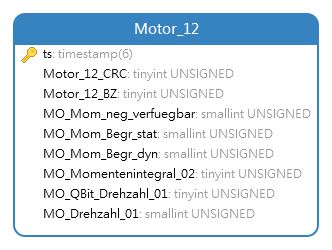
\includegraphics[width=0.3\textwidth]{gfx/mysql_model.png}
    \caption{DTable structure of Motor\_12 in MySQL}
    \label{fig:mysql_model}
\end{figure}

The SQL code below will construct a MySQL schema for the supplied model.

\begin{minted}[
frame=lines,
framesep=2mm,
baselinestretch=1.2,
bgcolor=LightGray,
fontsize=\footnotesize,
linenos
]{bash}
CREATE TABLE audi_a8.`Motor_12`  (
  `ts` timestamp(6) NOT NULL,
  `Motor_12_CRC` tinyint UNSIGNED NULL DEFAULT NULL,
  `Motor_12_BZ` tinyint UNSIGNED NULL DEFAULT NULL,
  `MO_Mom_neg_verfuegbar` smallint UNSIGNED NULL DEFAULT NULL,
  `MO_Mom_Begr_stat` smallint UNSIGNED NULL DEFAULT NULL,
  `MO_Mom_Begr_dyn` smallint UNSIGNED NULL DEFAULT NULL,
  `MO_Momentenintegral_02` tinyint UNSIGNED NULL DEFAULT NULL,
  `MO_QBit_Drehzahl_01` tinyint UNSIGNED NULL DEFAULT NULL,
  `MO_Drehzahl_01` smallint UNSIGNED NULL DEFAULT NULL,
  PRIMARY KEY (`ts`)
) ENGINE = InnoDB CHARACTER SET = utf8 KEY_BLOCK_SIZE = 8 ROW_FORMAT = Compressed;
\end{minted}

Data can be inserted into the database of MySQL in the following manner.
 
\begin{minted}[
frame=lines,
framesep=2mm,
baselinestretch=1.2,
bgcolor=LightGray,
fontsize=\footnotesize,
linenos
]{bash}
INSERT INTO `Motor_12` VALUES (1601199986097467, 248, 0, 510, 145, 509, 100, 0, 0);
\end{minted}

To query the data by time range
\begin{minted}[
frame=lines,
framesep=2mm,
baselinestretch=1.2,
bgcolor=LightGray,
fontsize=\footnotesize,
linenos
]{bash}
SELECT * FROM Motor_12 WHERE ts BETWEEN '2021-09-27 08:00:00' AND '2021-09-28 22:00:00'
\end{minted}

\subsection{InnoDB Storage Engine of MySQL}
For MySQL, it provides many types of storage engines, such as InnoDB, MyISAM, MEMORY, and MERGE. We can choose different storage engines according to our data processing needs. Here is the introduction of InnoDB, the most frequently used storage engine.

The data in mysql is stored on disk, and the real data processing is performed in memory. Since disk read and write speed is slow, if every operation reads and writes frequently to disk, then performance must be very poor. Therefore, InnoDB divides the data into pages and uses pages as the basic unit of interaction between disk and memory, and the general page size is 16KB. In this way, at least one page of data is read into memory or one page of data is written to disk at a time. By reducing the number of memory-disk interactions, thus improving performance. InnoDB tables arrange data on disk to optimize queries based on primary keys. Each table has a primary key index to organize data to minimize I/O for primary key query.


\paragraph{Storage of Data}

In the InnoDB storage engine, all data is logically stored in tablespace. Underneath the tablespace, there are segments, extents, pages (Figure \ref{fig:tablespaces}). By default, the page size in tablespaces is 16KB, but the default size can be changed by changing the innodb\_page\_size option\cite{mysql_innodb_parameter}. In the InnoDB storage engine, the minimum size of a extent is 1MB and the minimum number of pages is 64.

\begin{figure}[hbt!]
    \centering
    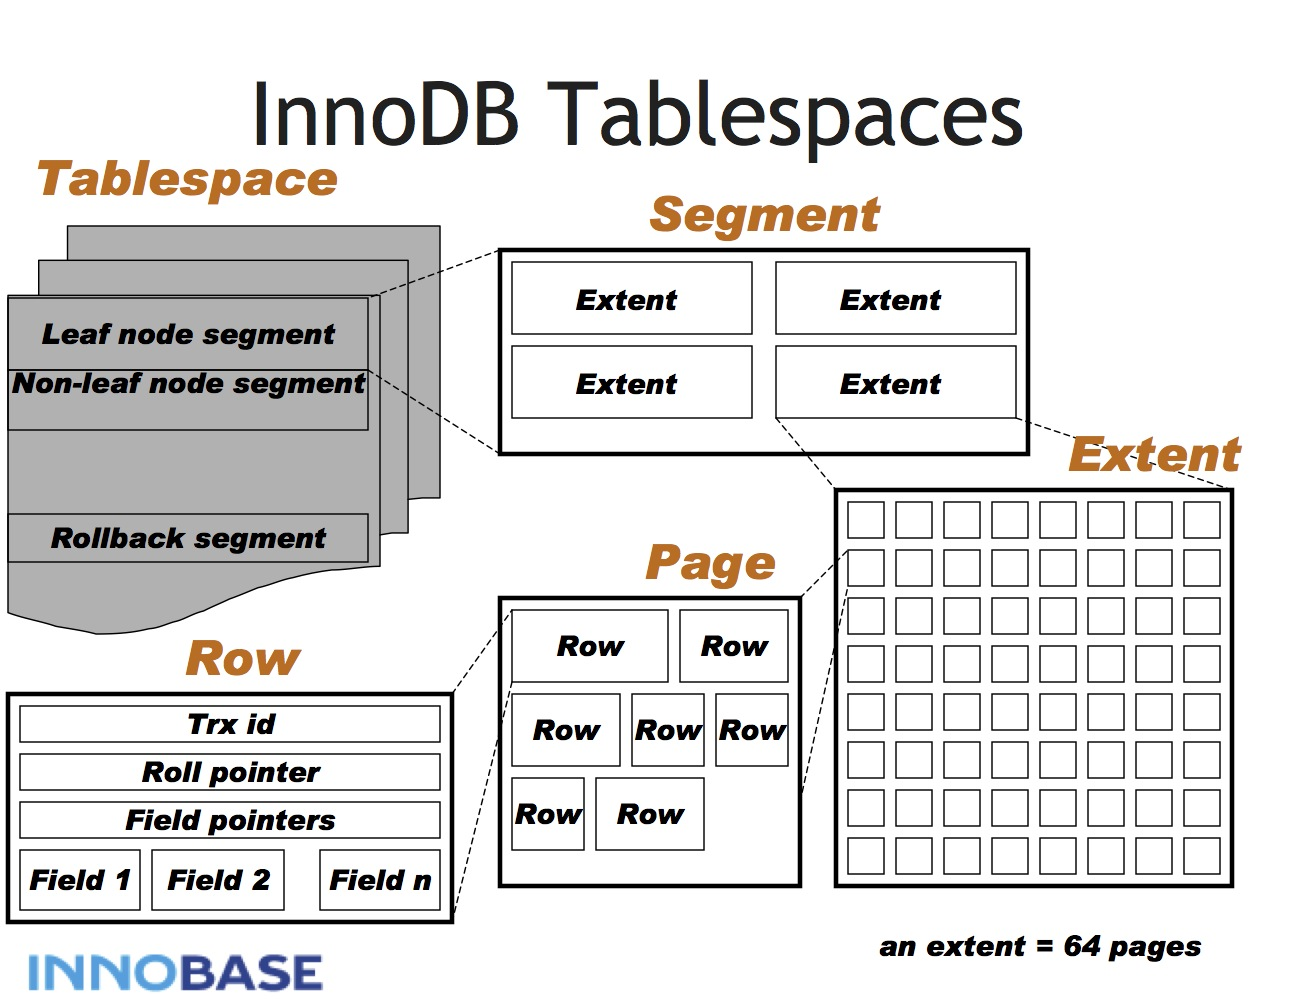
\includegraphics[width=0.6\textwidth]{gfx/table_space.jpg}
    \caption{InnoDB Tablespaces \cite{innodb}}
    \label{fig:tablespaces}
\end{figure}

\paragraph{How to store tables}

MySQL stores table definitions in .frm files and data indexes in .ibd files when using InnoDB to store tables. 

\paragraph{How to Store Records}

InnoDB uses pages as the smallest unit of disk management. Data is stored on a row-by-row basis in the InnoDB storage engine, and each 16KB page can hold 2-200 rows of records.

\paragraph{Data Page Structure}

Pages are the smallest disk unit of data managed by the InnoDB storage engine, and B-Tree nodes are the pages that actually hold the data in the table.

First, an InnoDB page has the following seven parts (Table \ref{tab:innodb_page}). Each page contains two pairs of header/trailer. The internal Page Header/Page Directory is concerned with page status information, while the File Header/File Trailer is concerned with recording page header information. Each data page contains two virtual records, Infimum and Supremum. Infimum record is a smaller value than any primary key value in the page, Supremum is the maximum value in the page\cite{mysql_page}. User Records is the part of the page that actually stores the row records, while Free Space is the empty space. It is a linked table data structure, in order to ensure the efficiency of insertion and deletion.

\begin{table}[hbt!]
\centering
\begin{tabular}{|c|}
\hline
File Header                 \\ \hline
Page Header                 \\ \hline
Infilmum + Supremum Records \\ \hline
User Records                \\ \hline
Free Space                  \\ \hline
Page Directory              \\ \hline
File Trailer                \\ \hline
\end{tabular}
\caption{InnoDB Data Page Structure}
\label{tab:innodb_page}
\end{table}

\paragraph{Index}
Index optimization is the most effective way to optimize query performance, it can easily improve the performance of the query by several orders of magnitude. The InnoDB storage engine uses B+ tree indexes in most cases, which are the most common and effective indexes for relational database queries, but a B+ tree index does not find the specific value corresponding to a given key, it can only find the page corresponding to the data row. The database reads the entire page into memory and looks for the specific row of data in memory.  The B+ tree is chosen because of the small height of the tree, which makes querying more efficient. Typically 20 million data, using the B+tree index, three disk IOs will be able to check the corresponding data\cite{mysql_page}.

\paragraph{Data writing process}
First of all, when the data is to be written or modified, you must first check to find the page where the data is located. If the page is not located in the buffer pool, a missing page interrupt will occur and the page on disk will be loaded into the buffer pool. After finding the page, the current data must be saved to the undo log, so that the data can be rolled back after the transaction is rolled back. After that, the data on the page will be modified directly and recorded in the redo log buffer\cite{mysql_page}.


\section{ClickHouse}

ClickHouse is an open-source column-oriented \ac{dbms} for OLAP. ClickHouse's most prominent feature is its lightning-fast query processing and data storage efficiency.

The characteristics of ClickHouse are shown below:

\begin{itemize}
    \item True Column-Oriented Database: No extra data is stored with the values which is different from HBase, Cassandra and BigTable\cite{clickhouse_feature}.
    \item Data compression: Each column of data can be compressed according to a specific algorithm, such as lz4 or delta-of-delta.
    \item Vector Computation Engine: Data is not only stored in columns, but it is also processed in vectors, allowing for maximum \ac{cpu} efficiency\cite{clickhouse_feature}.
    \item Parallel Processing on Multiple Cores: Large searches are inherently parallelized, using all of the available resources on the server\cite{clickhouse_feature}.
    \item SQL support: A declarative query language based on SQL is supported by ClickHouse\cite{clickhouse_feature}.
\end{itemize}

\subsection{Data Modelling in ClickHouse}

\begin{figure}[hbt!]
    \centering
    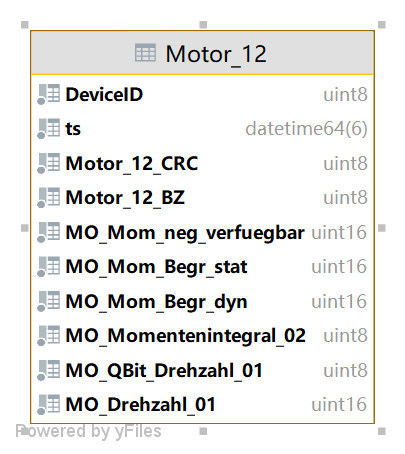
\includegraphics[width=0.3\textwidth]{gfx/Motor_12_ch.png}
    \caption{Table structure of Motor\_12 in ClickHouse}
    \label{fig:ch_model}
\end{figure}

Only the MergeTree family of table engines supports primary key indexes, data partitioning, data replicas, and data sampling. ReplacingMergeTree is distinguished from MergeTree in that it eliminates duplicate entries with the same sorting key value\cite{mergetree_clickhouse}. The sorting key (ORDER BY) is used to specify the criteria by which data is sorted within a data segment, which is the primary key by default. Here the timestamp is still used as the primary key. The SQL code below will construct a ClickHouse schema for the supplied model.

\begin{minted}[
frame=lines,
framesep=2mm,
baselinestretch=1.2,
bgcolor=LightGray,
fontsize=\footnotesize,
linenos
]{bash}
create table audi_a8.Motor_12
(
    DeviceID               UInt8,
    ts                     DateTime64(6),
    Motor_12_CRC           UInt8,
    Motor_12_BZ            UInt8,
    MO_Mom_neg_verfuegbar  UInt16,
    MO_Mom_Begr_stat       UInt16,
    MO_Mom_Begr_dyn        UInt16,
    MO_Momentenintegral_02 UInt8,
    MO_QBit_Drehzahl_01    UInt8,
    MO_Drehzahl_01         UInt16
)
    engine = ReplacingMergeTree(DeviceID)
        ORDER BY ts
        SETTINGS index_granularity = 8192;
\end{minted}

Similar to MySQL data can be inserted into the database of ClickHouse in the following manner.
\begin{minted}[
frame=lines,
framesep=2mm,
baselinestretch=1.2,
bgcolor=LightGray,
fontsize=\footnotesize,
linenos
]{bash}
INSERT INTO `Motor_12` VALUES (1, 1601199986097467, 248, 0, 510, 145, 509, 100, 0, 0);
\end{minted}

To query the data by time range
\begin{minted}[
frame=lines,
framesep=2mm,
baselinestretch=1.2,
bgcolor=LightGray,
fontsize=\footnotesize,
linenos
]{bash}
SELECT * FROM Motor_12 WHERE ts BETWEEN '2021-09-27 08:00:00' AND '2021-09-28 22:00:00'
\end{minted}

\subsection{Storage engine of ClickHouse}

The idea of MergeTree is similar to LSM-Tree. MergeTree sorts the written data first and then stores it. Each data partition in the MergeTree table's storage structure is independent of the others, with no logical links. A single partition contains multiple MergeTree Data Parts. The following Figure \ref{fig:ch_structure} shows the logic of the MergeTree storage structure of the table.

\begin{figure}[hbt!]
	\centering
 	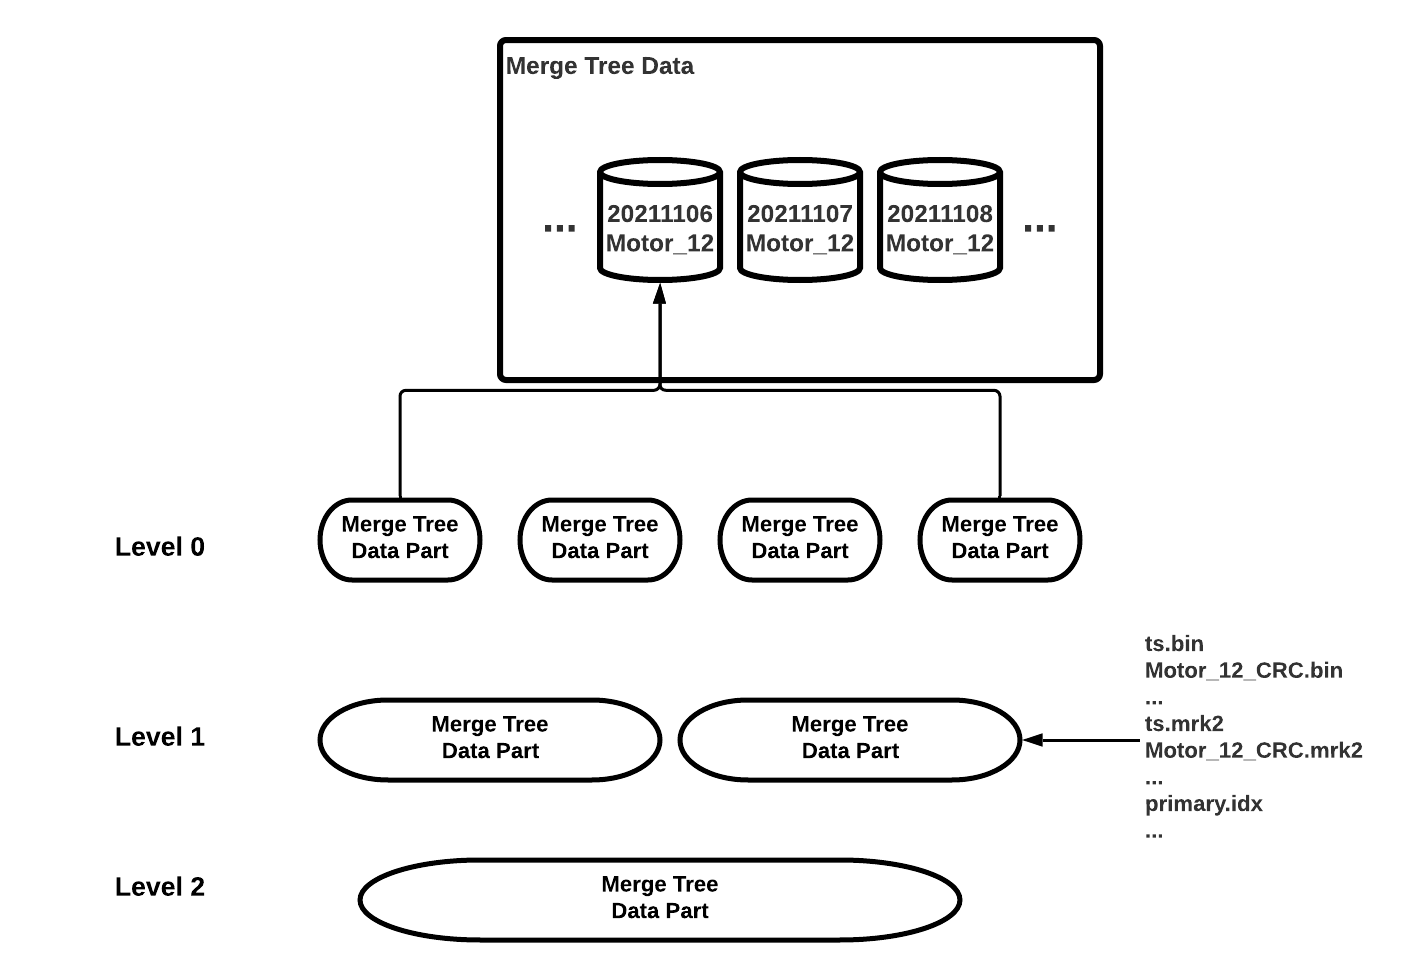
\includegraphics[width=0.8\textwidth]{gfx/ch_structure.png}
	\caption{MergeTree storage structure}
	\label{fig:ch_structure}
\end{figure}


Once generated, these Data Parts are Immutable. The MergeTree table write link is a batch load process, and the Data Part does not support a single append insert \cite{alibaba_cloud_community}. Each batch insert generates a new MergeTree Data Part. If only one row is inserted at a time, a separate Data Part is created for that row as well. This has a significant impact on the speed of merging later. So in general, batch insert (>1000 rows) is reasonable for MergeTree. There are three main categories in terms of functionality.

\begin{figure}[hbt!]
	\centering
 	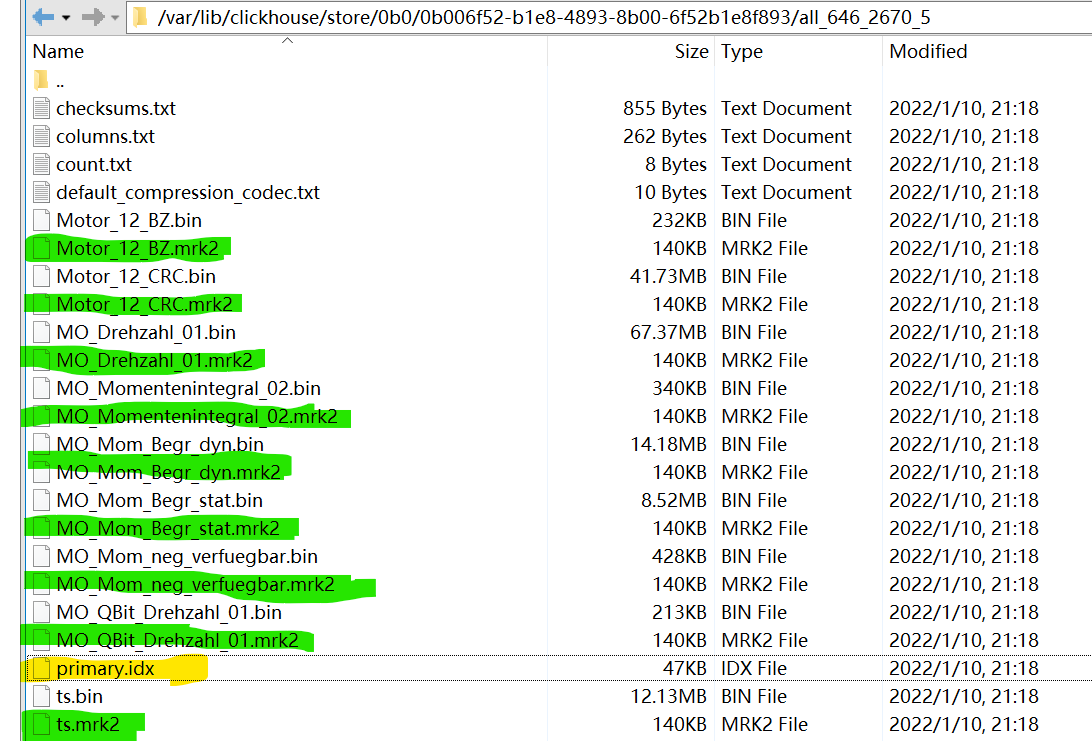
\includegraphics[width=0.8\textwidth]{gfx/ch_bin_mrk_idx.png}
	\caption{Primary Index, Data and Mark file in table of Motor\_12}
	\label{fig:motor_12_primary_mark}
\end{figure}

\begin{enumerate}

    \item Data files: 
    
    As shown in the Figure \ref{fig:ch_granule}, Motor\_12\_CRC.bin, MO\_Drehzahl\_01.bin, ts.bin, etc. are single column files compressed by block. The bin files are sorted and aligned by ts.bin because ts is the sorting key.
    
    \item Mark files:
    
    Motor\_12\_CRC.mrk2, MO\_Drehzahl\_01.mrk2, ts.mrk2, etc. are marks in the column storage files, and marks are related to two important concepts in MergeTree storage: Granule and Block.
    
    ClickHouse MergeTree divides bin files into granules according to their granularity. Each granule is compressed and stored separately. As shown in the Figure \ref{fig:ch_granule}, SETTINGS index\_granularity=3 means that every 3 rows of data is a granule, the partition currently has only 8 rows of data, so it is divided into 3 granules (three color blocks). To make it easier to read a granule, *.mrk file is used to record the offset of each granule, and some meta information is recorded in the header of each granule for reading\cite{alibaba_cloud_community}. So it is possible to locate the desired granule directly according to the mark file, and then read and verify the individual granule (Figure \ref{fig:ch_mark}).
    
    \begin{figure}[hbt!]
    \centering
    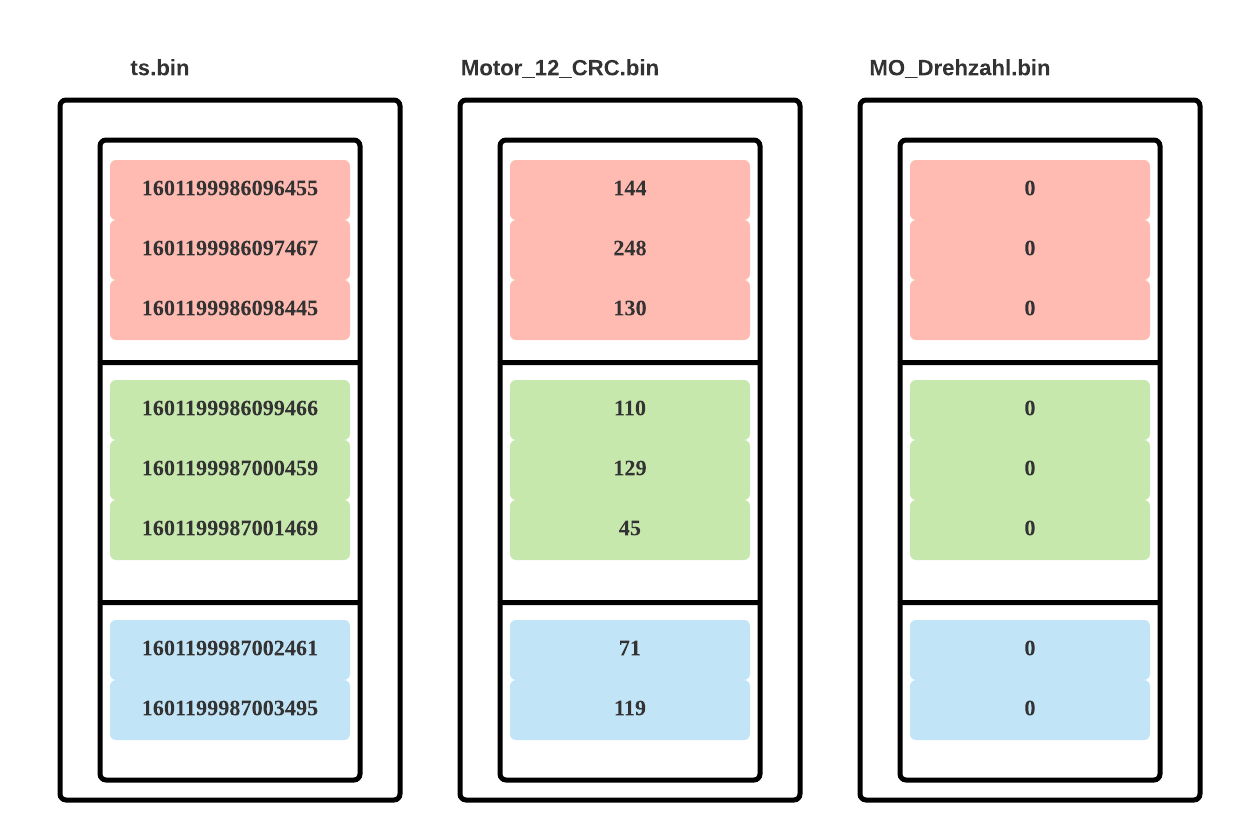
\includegraphics[width=0.6\textwidth]{gfx/bin_data_ch.png}
    \caption{bin data file with Granule}
    \label{fig:ch_granule}
    \end{figure}
    
        \begin{figure}[hbt!]
    \centering
    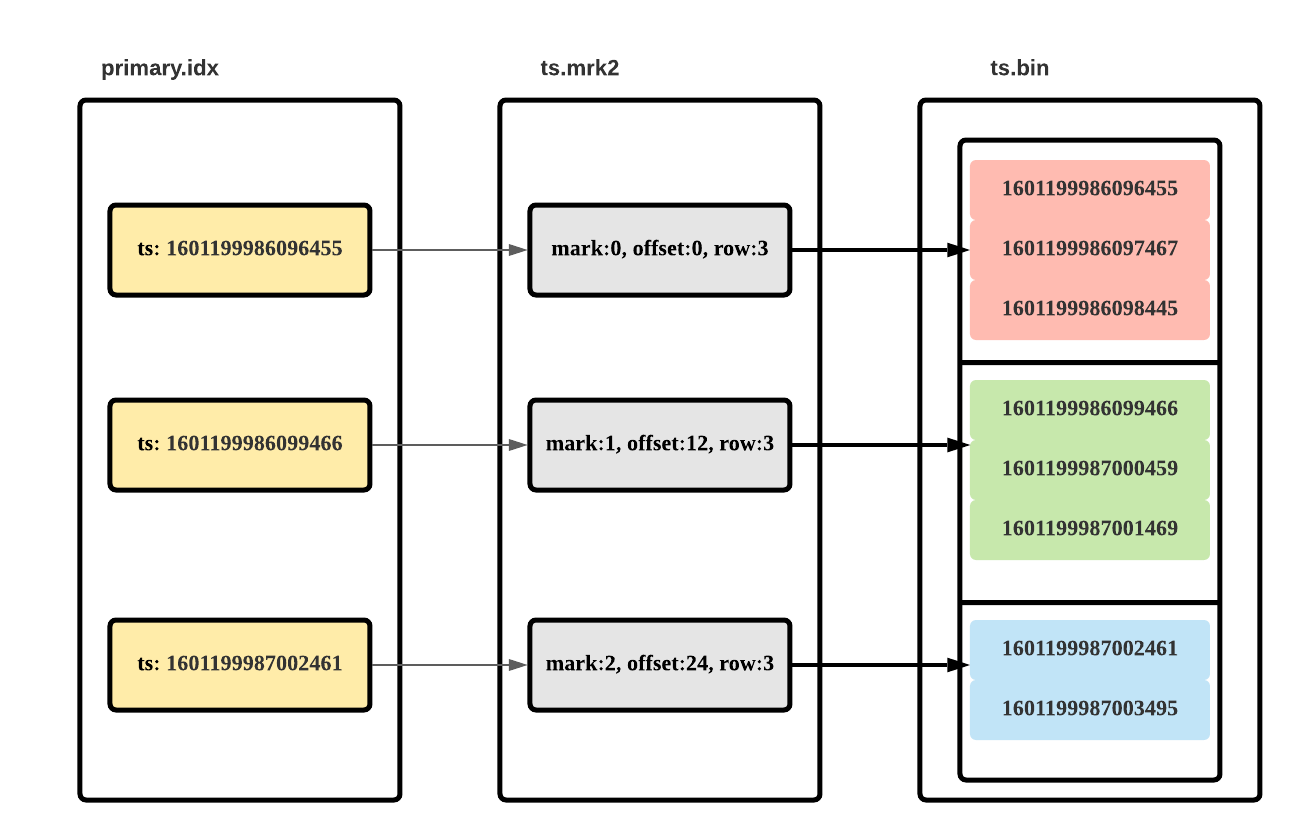
\includegraphics[width=0.7\textwidth]{gfx/mrk_primary_ch.png}
    \caption{bin data file with Marker, Primary key}
    \label{fig:ch_mark}
    \end{figure}

    
    Block is a compression unit in a column store file. Each block of a column store file contains several Granules, and the number of Granules is controlled by the parameter min\_compress\_block\_size. Each time a Granule is written in a block, it checks whether the current Block Size has reached the set value, and if so, the current block will be compressed and then written to disk.
    
    \item Primary Index
    
    In clickhouse's data storage file, the primary index is located in primary.idx.
    ClickHouse primary index is not the same concept as MySQL primary key.
    ClickHouse uses a sparse index, which selects points at intervals from the full amount of data that has been sorted and records which mark these points belong to. The primary key index can be specified by [PRIMARY KEY expr], the default is ORDER BY field value. In the selection of sparse points, the minimum value of each granule is taken. For example, a set of 50 million rows of data with a primary key ranging from 1 to 50,000,000 is stored in ClickHouse as a block of 8192 rows, so there are 6,101 blocks in total. The Index is 1, 8193, 16385 ......
    For instance, if a user needs to query for data with id > 10000 and id < 20000, then only block 1 (8193) and block 2 (16385) would be read. In addition, because the primary index is very small, with 100 million rows of data requiring just over 10,000 rows of index, the primary index can be resident in memory to speed up searching.
    
    
\end{enumerate}
Data query steps of MergeTree:
\begin{enumerate}
    \item Determine the partition (if any).
    \item Determine which blocks the data is in based on primary index (primary.idx).
    \item Determine exactly where the data is based on the data mark (.mrk2).
    \item Load data into memory and then query for filters.
\end{enumerate}

\section{Cassandra}

Cassandra is a NoSQL database management system that is open-source, distributed, and uses a wide-column store based on ideas of BigTable\cite{10.1145/1365815.1365816}. Because of its flexibility to scale both elastically and linearly, it is an excellent choice for storing large amounts of structured and unstructured data. Cassandra's main feature is that it is a distributed web service made up of a bunch of database nodes, with write operations to Cassandra being replicated to other nodes and read operations being routed to a node for reading. Scaling the performance of a Cassandra cluster is as simple as adding nodes to the cluster. Cassandra, like relational databases, implements ACID characteristics and has a fast write speed\cite{7507966}.

The characteristics of Cassandra are shown below:
\begin{itemize}
    \item Scalability: Cassandra is horizontally scalable. To add more capacity to the cluster, you can point to another new server.
    \item Multiple data centres: Distributed architectures are designed specifically for deployment across multiple data centers, redundancy, failover, and disaster recovery.
    \item Transaction support: Cassandra supports attributes such as atomicity, consistency, isolation and persistence (ACID).
    \item Flexible data storage: Cassandra supports all possible data formats, including structured, semi-structured and unstructured.
    \item Convenient data distribution: Cassandra has the flexibility to distribute data as needed because it replicates data across multiple data centers.
    \item \ac{cql}: As an alternative to traditional SQL, CQL offers an interface for querying Cassandra\cite{cassandra_wikipedia_2021}. 
\end{itemize}

\subsection{Data Modelling in Cassandra}

This is one of the most basic methods for storing time series data. For each CAN-ID, a wide row of data is created. The row key is a unique device identifier, such as Datalogger\_1, and the column name is the timestamp at which the data was recorded. The parsed data will be the value stored in these columns (Figure \ref{tab:cassandra_model}).

\begin{table}[hbt!]
\centering
\resizebox{\textwidth}{!}{%
\begin{tabular}{|ccccccc|}
\hline
\multicolumn{1}{|c|}{\multirow{2}{*}{\begin{tabular}[c]{@{}c@{}}Device\\ ID\end{tabular}}} &
  \multicolumn{1}{c|}{Timestamp} &
  \multicolumn{1}{c|}{Motor\_12\_CRC} &
  \multicolumn{1}{c|}{MO\_Mom\_neg\_verfuegbar} &
  \multicolumn{1}{c|}{MO\_Mom\_Begr\_stat} &
  \multicolumn{1}{c|}{MO\_Mom\_Begr\_dyn} &
  \multirow{2}{*}{...} \\ \cline{2-6}
\multicolumn{1}{|c|}{} &
  \multicolumn{1}{c|}{value1} &
  \multicolumn{1}{c|}{value2} &
  \multicolumn{1}{c|}{value3} &
  \multicolumn{1}{c|}{value4} &
  \multicolumn{1}{c|}{value5} &
   \\ \hline
\multicolumn{7}{|c|}{...} \\ \hline
\end{tabular}%
}
\caption{Storing the data for Motor\_12 per row}
\label{tab:cassandra_model}
\end{table}

\ac{cql} code below will construct a Cassandra schema for the supplied model.

\begin{minted}[
frame=lines,
framesep=2mm,
baselinestretch=1.2,
bgcolor=LightGray,
fontsize=\footnotesize,
linenos
]{bash}
CREATE TABLE Motor_12(
  deviceID text,
  ts timestamp,
  Motor_12_CRC tinyint,
  Motor_12_BZ tinyint,
  MO_Mom_neg_verfuegbar smallint,
  MO_Mom_Begr_stat smallint,
  MO_Mom_Begr_dyn smallint,
  MO_Momentenintegral_02 tinyint,
  MO_QBit_Drehzahl_01 tinyint,
  MO_Drehzahl_01 smallint,
  PRIMARY KEY(deviceID,ts)
) WITH compression = {'class': 'LZ4Compressor'};
\end{minted}

The following CQL statement is used to query the data by device id and time range.

\begin{minted}[
frame=lines,
framesep=2mm,
baselinestretch=1.2,
bgcolor=LightGray,
fontsize=\footnotesize,
linenos
]{bash}
SELECT * FROM Motor_12 
WHERE deviceID='Datalogger_1' 
AND ts BETWEEN '2021-09-27 08:00:00' AND '2021-09-28 22:00:00'
\end{minted}

\subsection{Storage Engine of Cassandra}
Cassandra first writes client-submitted data and operation records to commitLog, which aims to improve reliability and play the role of data recovery. Then cassandra writes the data to the memtable, which is an in-memory table where the data is organized by key. When the data in memtable reaches a certain limit (periodic/batch), it is flushed to an SSTable. The goal is to replace random IO writes with sequential IO writes, which greatly reduces the stress of write operations on the storage system. 

After the SSTable is successfully written, it cannot be changed and can only be read, so for Cassandra, there are only sequential writes and no random writes. Because of the read-only character of SSTbale, the data of the same Column Family may be stored in multiple SSTables. If the amount of data in a Column Family is very large, Cassandra will combine and read multiple SSTables and Memtable, causing the query efficiency to be seriously reduced\cite{cassandra_write}. Therefore, Cassandra uses BloomFilter, a data structure stored in memory, to quickly determine whether a given key is located in an SSTable so that Cassandra can quickly locate the SSTable corresponding to a key.

To avoid the performance impact of having a large number of SSTables, Cassandra handles SSTables that are expanding over time through a mechanism called Compaction.
Cassandra periodically merges multiple SSTables into a single SSTable, and since the data in each SSTable is ordered, the task can be accomplished by doing a single merge sort\cite{compaction_cassandra}.

\begin{figure}[hbt!]
    \centering
    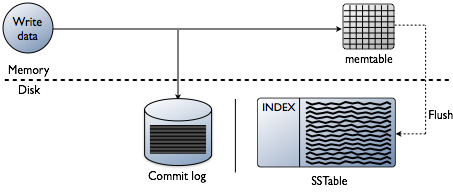
\includegraphics[width=0.5\textwidth]{gfx/cassandra_storage.png}
    \caption{Storage Engine of Cassandra \cite{cassandra_write}}
    \label{fig:storage_cassandra}
\end{figure}

In Cassandra's data storage directory, there are three types of files that can be found, Index.db, Filter.db, and Data.db (Figure \ref{fig:file_cassandra}). The Data.db file is the SSTable data file. Index.db is the index file, which holds the offset position of each key in the data file. Filter.db is the mapping file produced by the Bloom Filter algorithm\cite{compaction_cassandra}.

\begin{figure}[hbt!]
    \centering
    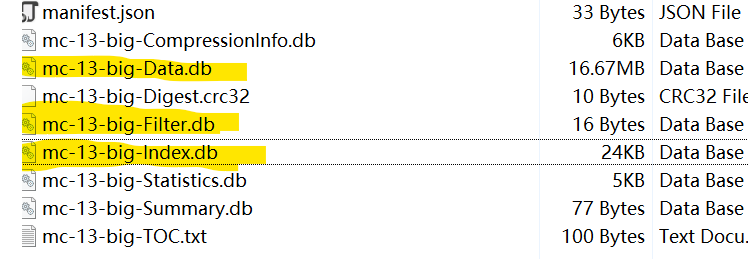
\includegraphics[width=0.4\textwidth]{gfx/file_cassandra.png}
    \caption{Data storage files of Cassandra}
    \label{fig:file_cassandra}
\end{figure}

\section{InfluxDB}
InfluxDB is an open-source time-series database developed by InfluxData and widely used for monitoring data in storage systems, real-time data in the IoT industry, and other scenarios\cite{influxdb_features}. InfluxDB is ranked No. 1 (Figure \ref{fig:database_ranking}) in DB-Engines' Time Series Database category.

The characteristics of InfluxDB are shown below:
\begin{itemize}
    \item Fast write performance: The underlying TSM storage engine, which is also based on the LSM idea, provides extremely strong write capabilities and high compression rates.
    \item Efficient query: Tags will be indexed to provide efficient query.
    \item Continuous Queries: Continuous queries automatically compute aggregate data to make frequent queries more efficient\cite{influxdb_features}.
    \item Retention policies: Fast deletion of out-of-date data.
    \item \ac{influxql}: Provides SQL-Like query language, which is convenient to use.
\end{itemize}

\subsection{Data modelling in InfluxDB}
In InfluxDB, time-series data supports a multi-value model with a point-in-time data\cite{alibaba_influxdb}.

\begin{figure}[hbt!]
	\centering
 	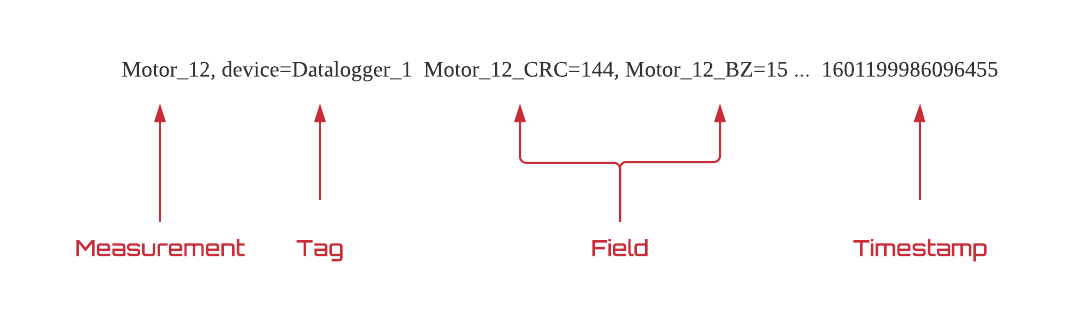
\includegraphics[width=0.8\textwidth]{gfx/influxdb_model.png}
	\caption{Data model of InfluxDB}
	\label{fig:influxdb_datamodel}
\end{figure}


\begin{enumerate}
    \item Measurement: 
    The measurement name is a description of the data recorded in the related fields, and the measurement works as a container for tags, fields, and the time column\cite{influxdb_glossary}. The names of CAN-IDs are used as the measurement.
    
    \item Tag:
    The key-value pair in an InfluxDB data structure that records metadata and the actual data value\cite{influxdb_glossary}. The Datalogger ID is used as Tag.
    \item Field:
    The specific metric value recorded by the data source, which is the data of each column after we parse it out.
    \item Timestamp: 
    Timestamp of each Trace
\end{enumerate}

Data can be inserted into the database of InfluxDB in the following manner. Since InfluxDB is a schemaless database, there is no need to define the structure in advance.

\begin{minted}[
frame=lines,
framesep=2mm,
baselinestretch=1.2,
bgcolor=LightGray,
fontsize=\footnotesize,
linenos
]{bash}
INSERT Motor_12,device=Datalogger_1 Motor_12_CRC=144,Motor_12_BZ=15,MO_Mom_neg_verfuegbar=510,
MO_Mom_Begr_stat=145,MO_Mom_Begr_dyn=509,MO_Momentenintegral_02=100,
MO_QBit_Drehzahl_01=0,MO_Drehzahl_01=0 
1601199986096455
\end{minted}

To query the data by time range
\begin{minted}[
frame=lines,
framesep=2mm,
baselinestretch=1.2,
bgcolor=LightGray,
fontsize=\footnotesize,
linenos
]{bash}
SELECT * FROM "Motor_12" WHERE time > now() - 1h
\end{minted}

\subsection{Storage Engine of InfluxDB}
Similar to the LSM structure, InfluxDB writes time series data into WALs, then cache, before flushing the disk to assure data integrity and availability. The process is shown in the following diagram (Figure \ref{fig:procedures_influxdb}). Serieskey data and time series data are segregated and written into distinct WALs (WALs of Index Data and WALs of Time Series Data). 

\begin{figure}[hbt!]
	\centering
 	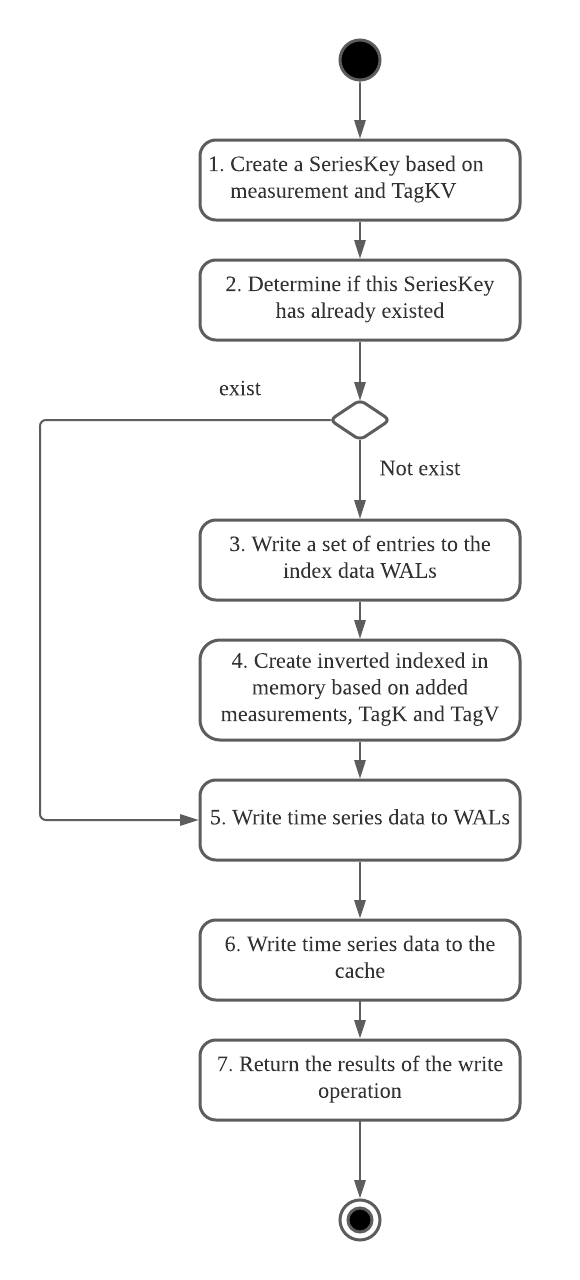
\includegraphics[width=0.3\textwidth]{gfx/procedure_influxdb.png}
	\caption{Procedures for writing time series data}
	\label{fig:procedures_influxdb}
\end{figure}

\paragraph{TSM}
When the data in the WAL exceeds the threshold, the WAL file is written to the level 1 TSM (Time Series Merge Tree) file and the cache and WAL are emptied\cite{alibaba_influxdb}. The storage structure of TSM is depicted in the Figure \ref{fig:structure_tsm} below. Each TSM file is divided into two main parts: the time-series data, and the index of the time-series data, which can be used to find the data needed using a binary search. As the number of TSM files grows, the system will merge several small TSM files into one larger TSM file, just like the LSM. The reason for this design is that when querying time series data, it is usually filtered by time, and most of the time the older the TSM file is, the older the data is, so the data is naturally sorted by time.

\begin{figure}[hbt!]
	\centering
 	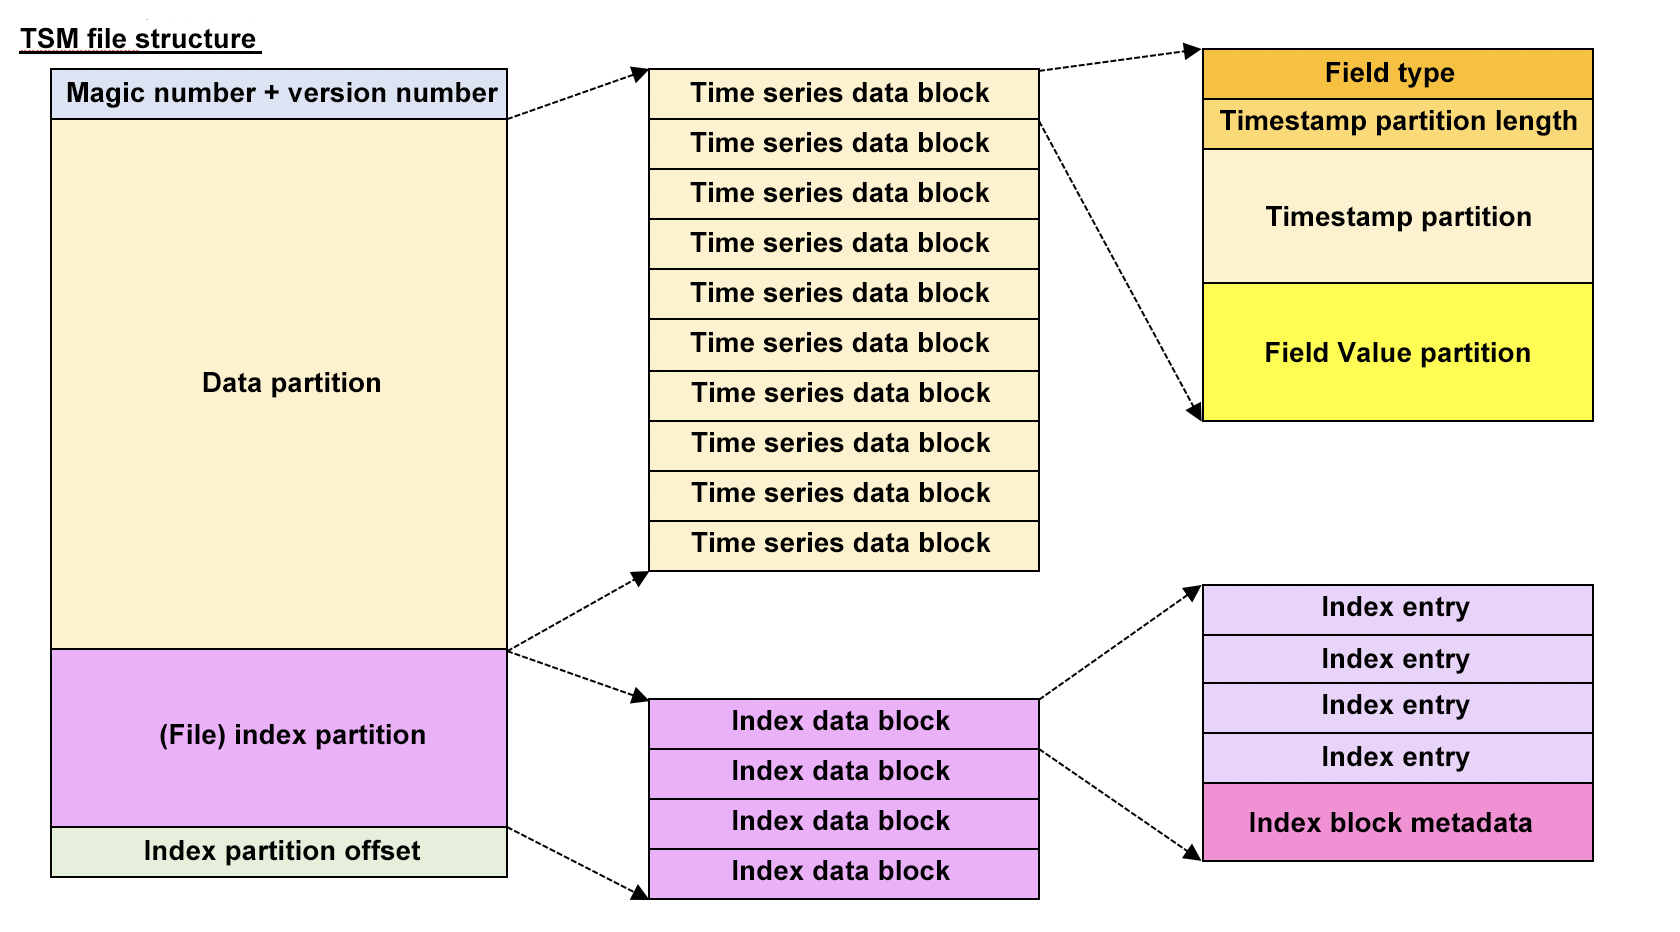
\includegraphics[width=0.5\textwidth]{gfx/TSM.png}
	\caption{Storage structure of TSM file\cite{alibaba_influxdb}}
	\label{fig:structure_tsm}
\end{figure}


\paragraph{TSI}
TSI is short for Time Series Index and is used by InfluxDB to keep an inverted index of time-series data. TSI can be used to quickly find out which series contain a certain tag in a particular table\cite{alibaba_influxdb}. The other task of the TSI is to store the inverted index on disk. In previous versions, influxdb uses in-memory storage for inverted index\cite{influxdb_cite}. When there is a very large amount of time-series data, the memory consumption of inverted indexes can spike.




%*****************************************
\chapter{Database performance comparison}
\label{ch:database_performancecomparison}
%*****************************************
This chapter compares read and write performance tests on several databases, namely MySQL, ClickHouse, Cassandra, and InfluxDB, mentioned in the previous chapters \ref{ch:choice_of_databases}.

\section{Test environment and step description}

The database versions are shown in the Table \ref{tab:version_database}.

\begin{table}[hbt!]
\centering
\begin{tabular}{@{}ll@{}}
\toprule
Database           & Version    \\ \midrule
MySQL      & 8.0.27     \\
ClickHouse & 21.11.4.14 \\
Cassandra  & 3.9.0      \\
InfluxDB   & 1.8.10     \\ \bottomrule
\end{tabular}
\caption{Version of Database}
\label{tab:version_database}
\end{table}

The comparison tests for all databases were performed on the same server, which was configured in detail as follows. 
\begin{table}[hbt!]
\centering
\begin{tabular}{@{}ll@{}}
\toprule
Configuration           & Version    \\ \midrule
CPU      & Intel(R) Xeon(R) Silver 4210   \\
RAM & 64 GB \\
hard disk  & 2 TB      \\
Operating System   & Ubuntu 18.04 x64     \\ \bottomrule
\end{tabular}
\caption{Configuration}
\label{tab:configuration}
\end{table}

The application and database are both operated on the same server to eliminate the effects of network latency. For the reliability of the data, each operation is repeated 10 times for both writes and queries and the final result is averaged. The database service is restarted before each test with a different database to avoid caching effects on the results obtained from previous executions.



From the DBC file, the corresponding tables are created in each database and each table is associated with a CAN ID. The exception is InfluxDB, which does not create tables (Measurements) in advance, as it is a schemaless database. The test data is CAN bus data, collected from the Audi A8 by ZD-Datalogger and stored as binary files in the HDFS distributed storage system.
The CAN bus data in HDFS is parsed by Spark and then written to the databases, each of which will use its own \ac{jdbc}. See Appendix \ref{lst:maven} for detailed information.

\begin{table}[hbt!]
\centering
\begin{tabular}{@{}ll@{}}
\toprule
\textbf{Criteria}       & \textbf{Weight} \\ \midrule
Write performance       & 25              \\
Read performance        & 20              \\
Aggregation performance & 20              \\
Disk usage              & 25              \\
Flexibility of database & 10              \\ \hline
\textbf{Sum}          & 100             \\ \bottomrule
\end{tabular}
\caption{Evaluation criteria with weighting}
\label{tab:evaluation_weight}
\end{table}

Comparisons between databases are made using the \ac{wsm}. Five comparison criteria, indicated by the rows in Table \ref{tab:evaluation_weight}, constitute the foundation. Each of these criteria is discussed in detail, as well as the weighting that was decided. This is followed by an analysis of each database in terms of this criterion, with each database receiving a final score (1-5). Table \ref{tab:rating_scale} shows the detailed classification. The weighting of the criterion was then multiplied by the results of this evaluation. The sum of the weighted values represents the final result, where the database with the highest score is considered to be the most appropriate.

\begin{table}[hbt!]
\centering
\begin{tabular}{|l|l|}
\hline
Very bad  & 1 \\ \hline
Bad       & 2 \\ \hline
Medium    & 3 \\ \hline
Good      & 4 \\ \hline
Very good & 5 \\ \hline
\end{tabular}
\caption{Rating scale}
\label{tab:rating_scale}
\end{table}

\section{Write performance comparison}

The database must first have the ability to write large amounts of data quickly, as CAN bus data can often be in the tens or even hundreds of millions of rows a day. If the user has to wait for a long time for the data to be written to the database, it will greatly affect the experience. So the score for write performance is up to 25.

The database may handle numerous client connections, and the overall insert throughput improves as the number of links grows. As a result, one client and numerous client connections are checked for each database in the test. One or more records can be included in a write request to the database. The write performance of most databases improves as the number of records in a request increases.

\begin{enumerate}
\item MySQL

\begin{itemize}
    
\item Adjusting database parameters

\begin{enumerate}
\item innodb\_flush\_log\_at\_trx\_commit=0

This parameter controls the durability/speed trade-off for commits. Set to 0 (write and flush redo log to disk only once per second), 1 (flush to disk at each commit), 2 (write to log at commit but flush to disk only once per second)\cite{mariadb}. 

The default value of this parameter is 1. For faster writing speed, the value of this parameter is changed to 0.
\item max\_allowed\_packet=128M

MySQL limits the packet size that Server accepts according to the configuration file. Sometimes large inserts and updates will be limited by this parameter, causing large data writes or updates to fail.

\item innodb\_autoextend\_increment=128M

This parameter is mainly used when the tablespace space is full, the MySQL system needs to automatically expand the amount of space, each time the tablespace expansion will make each SQL in a waiting state. Increasing the auto-extend size can reduce the number of times tablespace is automatically extended\cite{mariadb_autoextend}.

\item innodb\_log\_file\_size=128M

This parameter sets the size of each log file in a log group\cite{mariadb_log_file_size}.

\item innodb\_buffer\_pool\_size = 512M

This parameter is used to cache the index and data in memory. Data reads and writes are faster in memory, reducing the need to read and write to disk.

\end{enumerate}

\item JDBC and connection pool

Spark uses MySQL JDBC driver to connect to MySQL database. In order to control the number of clients, Spark also needs to use database connection pooling technology. HikariCP JDBC connection pool is used here. MySQL JDBC batch data processing requires adding rewriteBatchedStatements=true to the JDBC connection. See the code in Code \ref{lst:mysql_cp} for details.

If the write operation of data needs to execute INSERT statement several times, but only the inserted value is different each time, MySQL server also needs to check the syntax format of SQL statement and compile it every time, which wastes too much time. When PreparedStatement is used, then only one syntax check and compilation of the SQL statement is performed, so it is more efficient.

\renewcommand{\lstlistingname}{Code} % Listing->Code
\begin{lstlisting}[caption=Create MySQL database connection pool instance, style=myScalastyle, label=lst:mysql_cp]
  def getDataSourceInstance: HikariDataSource = {
    if (instance == null) {
      try {
        val config = new HikariConfig
        config.setJdbcUrl(
          "jdbc:mysql://master:3306/audi_a8_test?" +
            "rewriteBatchedStatements=true&useSSL=false&serverTimezone=UTC")
        config.setMinimumIdle(5);           //minimum number of idle connection
        config.setMaximumPoolSize(5);      //maximum number of connection in the pool
        config.setConnectionTimeout(300000) //maximum wait milliseconds
        config.setMaxLifetime(0);       // maximum life time for each connection
        config.setIdleTimeout(0);       // max idle time for recycle idle connection
        instance = new HikariDataSource(config)
      } catch {
        case ex: Exception => println(ex)
      }
    }
    instance
  }
\end{lstlisting}

\item Write performance

\begin{table}[hbt!]
\centering
\begin{tabular}{@{}llllll@{}}
\toprule
Batch size & 1 Client & 2 Clients & 3 Clients & 4 Clients & 5 Clients \\ \midrule
10      & 3,813   & 5,454    & 5,982    & 6,126    & 6,248    \\
100        & 12,065   & 13,781    & 12,975    & 14,540    & 14,891    \\
1000       & 37,255   & 35,433    & 30,281   & 37,903    & 39,374   \\
10000       & 31,590   & 34,185    & 32,053   & 38,582    & 35,196  \\ \bottomrule
\end{tabular}%
\caption{MySQL Database Write Performance (Unit: Rows/Second)}
\label{tab:mysql-write-performance}
\end{table}

According to the table \ref{tab:mysql-write-performance}, the greater the batch size, the better the write performance of MySQL. However, when the number of bulk writes is larger than 1000, the write speed does not increase. Furthermore, increasing the number of client connections does not enhance the write speed significantly. MySQL's maximum write speed in this test is about 40,000 records/sec.

\end{itemize}

\item ClickHouse

\begin{itemize}
\item JDBC and connection pool


Similar to the MySQL database, the HikariCP JDBC connection pool is used here. 

The JDBC driver used is ClickHouse Native JDBC. It has the following two benefits over the official yandex/clickhouse-jdbc driver.

\begin{itemize}
\item[-] Data is organized and compressed in columnar format when writing\cite{clickhouse_jdbc}.
\item[-] Driver is implemented based on TCP protocol, which is more efficient than HTTP protocol\cite{clickhouse_jdbc}.
\end{itemize}

\item Write performance
\begin{table}[hbt!]
\centering
\begin{tabular}{@{}llllll@{}}
\toprule
Batch size & 1 Client & 2 Clients & 3 Clients & 4 Clients & 5 Clients \\ \midrule
1000       & 150,013  & 171,197  & 195,430   & 218,024   & 226,956   \\
5000       & 358,981  & 417,652  & 423,934   & 430,851   & 431,457   \\
10000      & 393,358  & 485,259  & 498,982   & 503,125   & 503,737   \\
20000      & 407,870  & 500,984  & 522,855   & 533,048   & 538,342   \\
30000      & 416,052  & 545,982  & 561,540   & 572,390   & 571,824   \\ \bottomrule
\end{tabular}
\caption{Write Performance of ClickHouse (Unit: Rows/Second)}
\label{tab:click_write}
\end{table}

ClickHouse officially recommends that each batch write should ideally be at least 1000 rows of data. ClickHouse write speed improves with the number of clients at initially, but after the number of client connections reaches a specific threshold, ClickHouse write speed plateaus. According to the table \ref{tab:click_write}, ClickHouse's maximum write speed in this test is about 580,000 records/sec.

\end{itemize}

\item Cassandra

\begin{itemize}
\item JDBC and connection pool

The JDBC driver uses the package provided by Datastax. The execution of a PreparedStatement is a two-step process. In the prepare phase the server parses the CQL statement and caches it. Each time an execute is called afterwards, the server does not need to parse the statement again, but instead takes the parsed result from the cache and executes it, thus reducing the parsing time. In addition concurrent asynchronous writes are the fastest way to write to a Cassandra cluster.

\item Write performance

\begin{table}[hbt!]
\centering
\begin{tabular}{@{}llllll@{}}
\toprule
Batch size & 1 Client & 2 Clients & 3 Clients & 4 Clients & 5 Clients \\ \midrule
10         & 13,860   & 25,879   & 38,471    & 46,298    & 52,035    \\
100        & 143,013   & 154,795  & 158,562   & 151,025   & 189,625   \\
1000       & 185,820   & 193,435  & 197,182   & 195,743   & 201,737  \\
10000      & 175,932    & 195,589 & 187,804 & 185,947 & 194,473 \\ \bottomrule
\end{tabular}
\caption{Write Performance of Cassandra (Unit: Rows/Second)}
\label{tab:cassandra_write}
\end{table}
The above statistics \ref{tab:cassandra_write} show that Cassandra's write speed increases as the number of batch requests increases. Cassandra's write performance is unaffected by the number of client connections when the batch size is big. Finally Cassandra's maximum write speed in this test is about 200,000 records/sec.

\end{itemize}

\item InfluxDB

\begin{itemize}
\item Optimize writes to InfluxDB
    
InfluxDB provides a data storage structure (Batch Points) to store records temporarily and then write them to the database through (Write) operations. To speed up InfluxDB writes and save network traffic, use gzip compression.

\item Write performance
\begin{table}[hbt!]
\centering
\begin{tabular}{@{}llllll@{}}
\toprule
Batch size & 1 Client & 2 Clients & 3 Clients & 4 Clients & 5 Clients \\ \midrule
10         & 3,892    & 6,790    & 10,319    & 13,662    & 16,251    \\
100        & 27,107   & 49,199   & 69,301    & 80,224    & 91,446    \\
1000       & 69,588   & 109,237  & 128,540   & 135,037   & 134,815   \\
10000      & 79,834   & 122,696  & 134,573   & 128,970   & 132,630   \\
20000      & 86,562   & 131,857  & 135,946   & 141,012   & 133,902  \\ \bottomrule
\end{tabular}
\caption{Write Performance of InfluxDB (Unit: Row/Second)}
\label{tab:influx_write}
\end{table}

InfluxDB's writing speed improves practically linearly with the number of client connections when the Batch size is minimal. When the number of Batch size is large, the write speed of InfluxDB increases with the number of clients at first, and then stops increasing. According to the table \ref{tab:influx_write}, ClickHouse's maximum write speed in this test is about 140,000 records/sec.
\end{itemize}

\item All Results

\begin{figure}[hbt!]
    \centering
    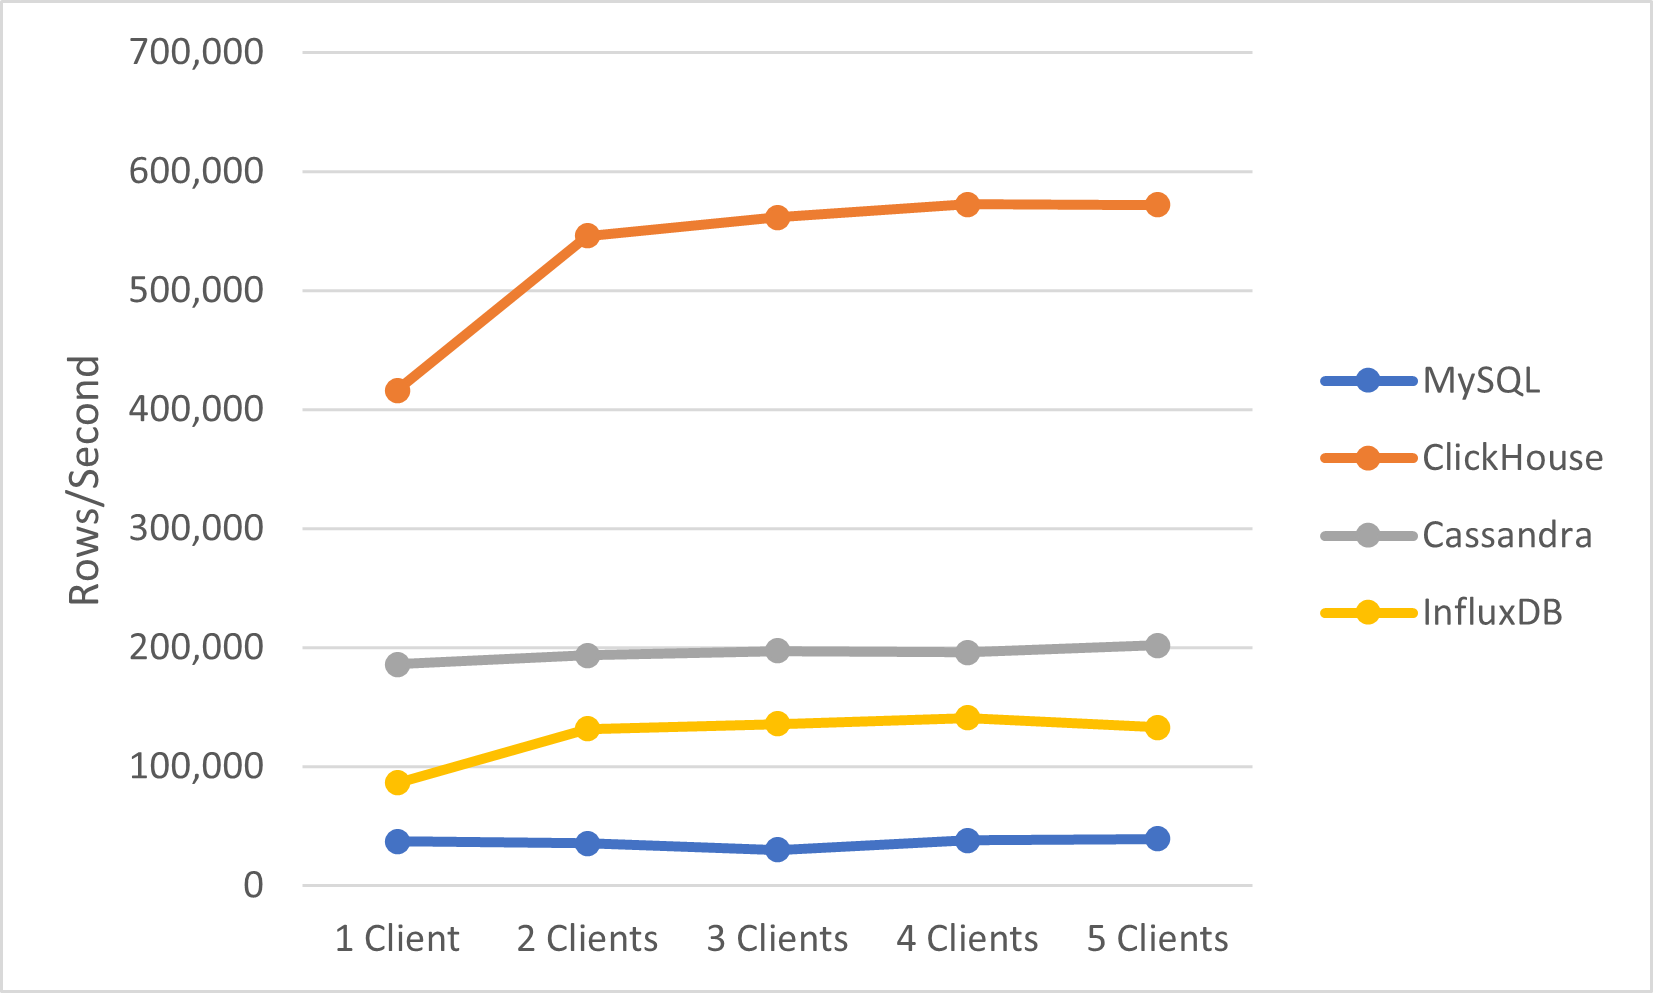
\includegraphics[width=0.6\textwidth]{gfx/all_write_perform.png}
    \caption{Comparison of all database write speeds}
    \label{fig:all_write}
\end{figure}

From the graphs \ref{fig:all_write} it can be concluded that the maximum throughput of ClickHouse is stable at about 500,000 records/sec, which is much faster than the second ranked Cassandra (about 200,000 records/sec). The maximum throughput of InfluxDB is around 132,000 records/second, and the last MySQL is 40,000 records/second. As a result, ClickHouse was rated very good, Cassandra was rated good, InfluxDB was rated medium and MySQL was rated bad in terms of write performance.

\end{enumerate}

\section{Read performance comparison}
Users often have the need to download the data in CAN-IDs according to the time period. So this requires the read performance of the database and the write performance for saving to CSV files. Therefore this score is 20.

This test reads out all the inserted data and exports the data as a csv file. The test code for different databases is shown below. The test data is the data in CAN bus Signal named Motor\_12 and total data volume is 50 million rows.

\begin{minted}[
frame=lines,
framesep=2mm,
baselinestretch=1.2,
bgcolor=LightGray,
fontsize=\footnotesize,
linenos
]{bash}
#MySQL
mysql mydb -e "SELECT * FROM audi_a8.Motor_12 WHERE ts BETWEEN ${time_start} AND ${time_end}" 
-B > motor_12_mysql.csv

#Clickhouse 
clickhouse-client --query "SELECT * FROM audi_a8.Motor_12 WHERE ts BETWEEN ${time_start} AND ${time_end}"
--format CSV > motor_12_ch.csv

#Cassandra
cqlsh −e"SELECT ∗ FROM audi_a8.motor_12 
WHERE deviceid='Datalogger1' AND ts BETWEEN ${time_start} AND ${time_end}"
> motor_12_cas.csv

#Influxdb
influx -database 'audi_a8' -execute 'SELECT * FROM Motor_12 
WHERE time > ${time_start} AND time < ${time_end}' -format csv > motor_12_influx.csv

\end{minted}
  
\begin{minipage}{\textwidth}
  \begin{minipage}[b]{0.49\textwidth}
    \centering
    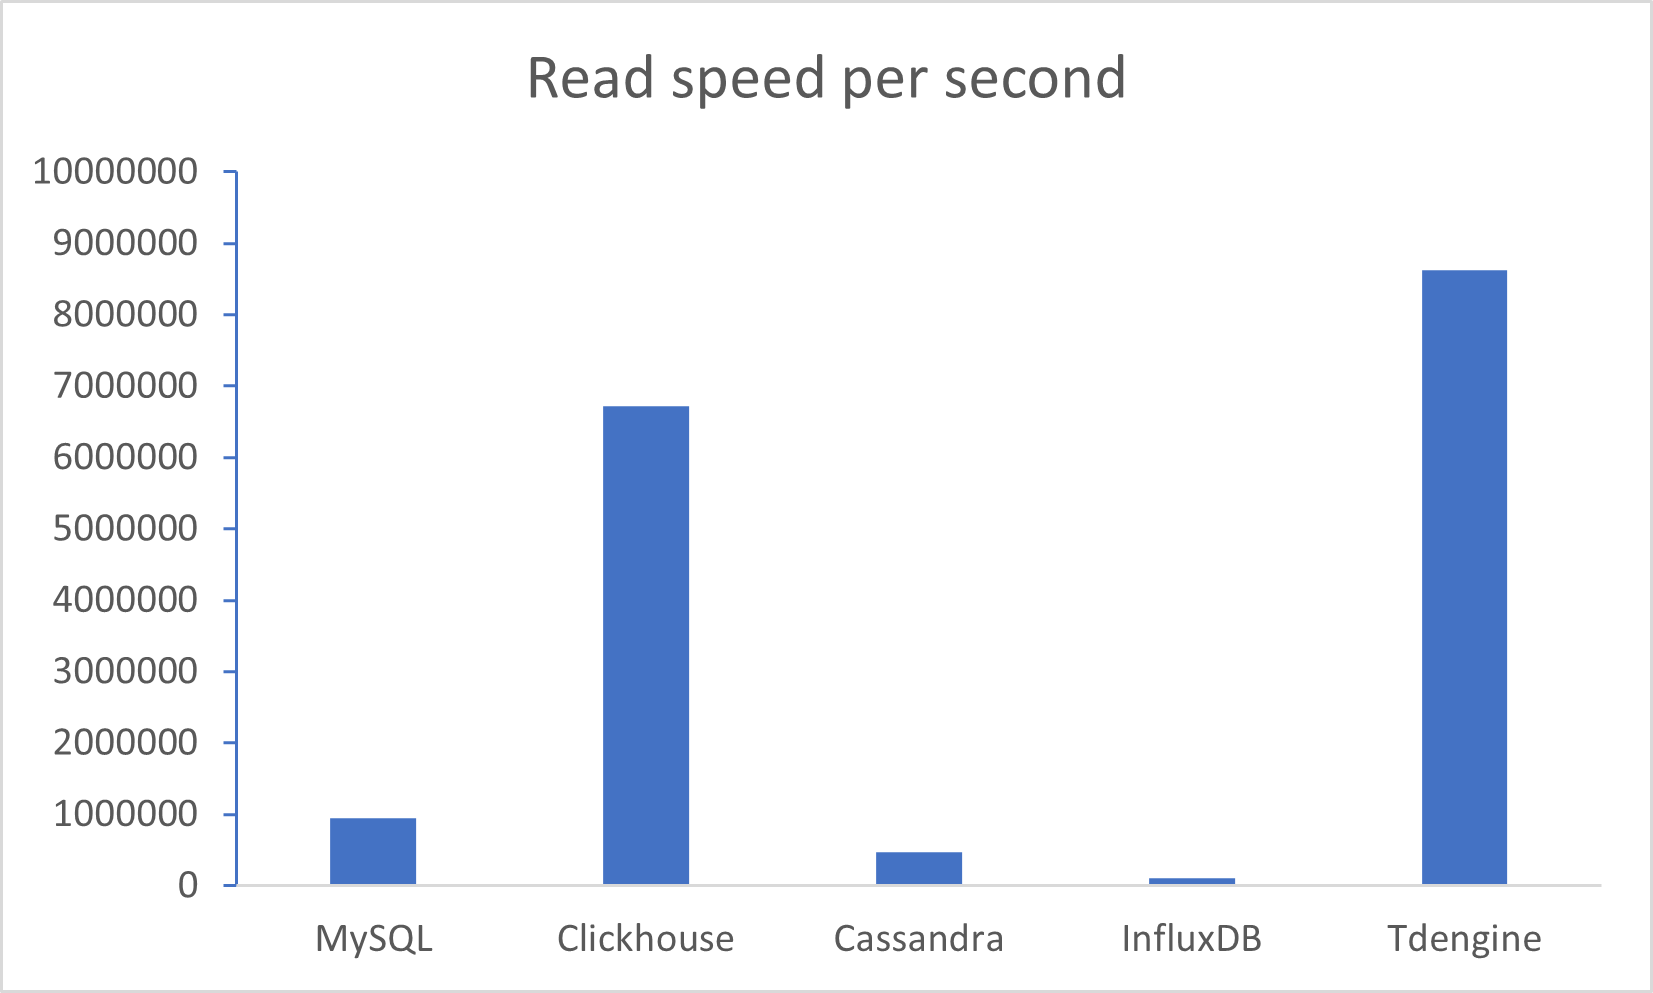
\includegraphics[width=0.9\textwidth]{gfx/read_performance.png}
    \captionof{figure}{Read performance}
    \label{fig:Read_performance}
  \end{minipage}
  \hfill
  \begin{minipage}[b]{0.49\textwidth}
    \centering
   \begin{tabular}{@{}ll@{}}
    \toprule
               & Rows read per second \\ \midrule
    MySQL      & 950,649               \\
    Clickhouse & 6,726,439             \\
    Cassandra  & 469,807               \\
    InfluxDB   & 108,921                \\ \bottomrule
    \end{tabular}
      \captionof{table}{Read performance statistics}
    \end{minipage}
  \end{minipage}
  
From the Figure \ref{fig:Read_performance}, it is concluded that ClickHouse can read more than 5 million rows of data per second. The read performance of the relational database MySQL is about 1 million rows per second. In contrast, Cassandra and InfluxDB reads are slower, below 500,000 rows per second. It should be noted that much of the CAN bus data is highly repetitive, so the compression of data in column databases like ClickHouse can be very high.  As a result, ClickHouse was rated very good, MySQL was rated good, Cassandra was rated medium and InfluxDB was rated bad in terms of read performance.

\section{Aggregation Performance comparison}
As mentioned in the previous Use Case chapter (Chapter \ref{use_case}), users usually need to aggregate queries on one or more columns of data for data visualization or data comparison. Therefore this score is 20.

Since the aggregation functions supported by different databases are not the same, this test contains COUNT, \ac{avg}, \ac{sum}, \ac{max}, \ac{min} five common aggregation functions. All of the test functions select rows from a single table or a single data collection point, with filter conditions (WHERE) if necessary, to confirm that the same rows are selected for different data models and databases.  The test data is the data in CAN bus Signal named Motor\_12. Each record has the following contents: timestamp, Motor\_12\_CRC (UInt8), Motor\_12\_BZ(UInt8), MO\_Mom\_neg\_verfuegbar (UInt16), MO\_Mom\_Begr\_stat (Uint16), MO\_Mom\_Begr\_dyn (UInt16), MO\_Momentenintegral\_02 (UInt8), MO\_QBit\_Drehzahl\_01 (UInt8), MO\_Drehzahl\_01 (UInt16). Because each database data model is unique, the data structure and settings for each database insert are not identical. The database is aggregated according to the time period, and there are different amounts of data for different time periods, 1 million, 10 million and 50 million rows of data respectively.

The following is the SQL code for MySQL aggregation query, and the SQL code for the rest of the database is shown in the Appendix \ref{lst: aggregate}.
\begin{minted}[
frame=lines,
framesep=2mm,
baselinestretch=1.2,
bgcolor=LightGray,
fontsize=\footnotesize,
linenos
]{bash}
# Aggregate query of MySQL 
SELECT COUNT(*) FROM audi_a8.Motor_12 WHERE ts BETWEEN ${time_start} AND ${time_end}
SELECT AVG(MO_Drehzahl_01) FROM audi_a8.Motor_12 WHERE ts BETWEEN ${time_start} AND ${time_end}
SELECT SUM(MO_Drehzahl_01) FROM audi_a8.Motor_12 WHERE ts BETWEEN ${time_start} AND ${time_end}
SELECT MAX(MO_Drehzahl_01) FROM audi_a8.Motor_12 WHERE ts BETWEEN ${time_start} AND ${time_end}
SELECT MIN(MO_Drehzahl_01) FROM audi_a8.Motor_12 WHERE ts BETWEEN ${time_start} AND ${time_end}
\end{minted}



\begin{table}[hbt!]
\centering
\begin{tabular}{@{}llll@{}}
\toprule
      & 1 million & 10 million & 50 million \\ \midrule
COUNT & 390       & 3,577       & 26,192      \\
AVG   & 819       & 4,862       & 24,817      \\
SUM   & 901       & 4,879       & 24,683      \\
MAX   & 461       & 4,231       & 24,228      \\
MIN   & 432       & 4,374       & 23,671      \\ \bottomrule
\end{tabular}
\caption{Aggregation Function of MySQL (Unit: milliseconds)}
\label{tab:agg_mysql}
\end{table}



\begin{table}[hbt!]
\centering
\begin{tabular}{@{}llll@{}}
\toprule
      & 1 million & 10 million & 50 million \\ \midrule
COUNT & 17        & 91         & 335        \\
AVG   & 25        & 97         & 397        \\
SUM   & 19        & 92         & 325        \\
MAX   & 22        & 92         & 331        \\
MIN   & 20        & 84         & 338        \\ \bottomrule
\end{tabular}
\caption{Aggregation Function of Clickhouse (Unit: milliseconds)}
\label{tab:agg_clickhouse}
\end{table}



\begin{table}[hbt!]
\centering
\begin{tabular}{@{}llll@{}}
\toprule
      & 1 million & 10 million & 50 million \\ \midrule
COUNT & 2,059      & 85,103      & 467,682     \\
AVG   & 2,390      & 87,934      & 483,641     \\
SUM   & 2,381      & 88,404      & 484,384     \\
MAX   & 2,287      & 89,963      & 490,102     \\
MIN   & 2,358      & 88,128      & 488,796     \\ \bottomrule
\end{tabular}
\caption{Aggregation Function of Cassandra (Unit: milliseconds)}
\label{tab:agg_cassandra}
\end{table}

\begin{table}[hbt!]
\centering
\begin{tabular}{@{}llll@{}}
\toprule
      & 1 million & 10 million & 50 million \\ \midrule
COUNT & 147       & 1,492       & 6,986       \\
AVG   & 145       & 1,466       & 6,404       \\
SUM   & 140       & 1,428       & 7,068       \\
MAX   & 167       & 1,599       & 7,072       \\
MIN   & 159       & 1,565       & 6,985       \\ \bottomrule
\end{tabular}
\caption{Aggregation Function of InfluxDB (Unit: milliseconds)}
\label{tab:agg_influx}
\end{table}


\begin{figure}[hbt!]
	\centering
 	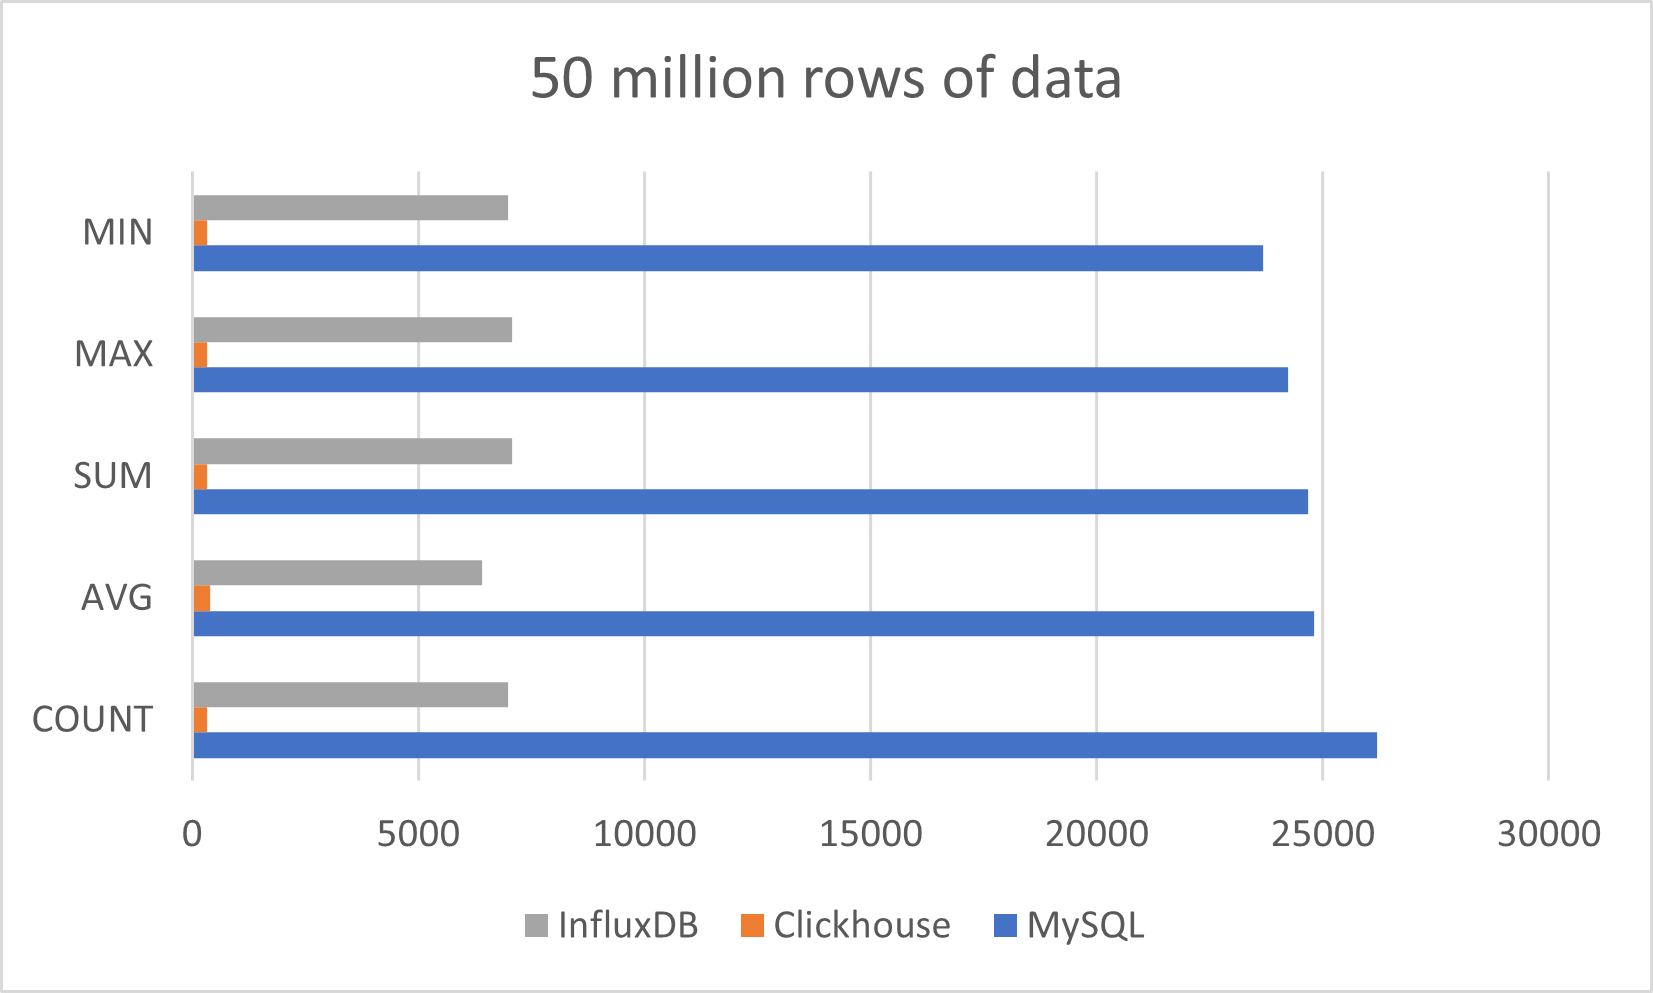
\includegraphics[width=0.7\textwidth]{gfx/agg_query.png}
	\caption{Aggregate query performance comparison}
	\label{fig:agg_performance}
\end{figure}

When querying a single data collecting point, ClickHouse has a benefit. In second place is InfluxDB, which is slower than ClickHouse in terms of query speed, but still significantly ahead of MySQL in third place. In the case of larger data volume, ClickHouse is 60 times faster than MySQL under aggregated queries. The above figure \ref{fig:agg_performance} does not include Cassandra's test results in order to maintain readability. Cassandra has the worst aggregation performance, so in general, Cassandra needs to work with Spark to complete aggregation queries for large data volumes. As a result, ClickHouse was rated very good, InfluxDB was rated good, MySQL was rated medium and Cassandra was rated bad in terms of aggregation performance.

\section{Downsampling Performance comparison}
Users sometimes need to perform downsampling queries. The time span is usually 1s, 10s, or 1 minute. However, not all databases have a syntax that supports downsampling query, and the only databases tested so far support downsampling queries are ClickHouse and InfluxDB. Therefore, this test does not count towards the total score.


Similar to the previous aggregate query test, the data volume is still 1 million, 10 million and 50 million according to the time period. The time intervals are 1s, 1 minute, and 1 hour, respectively.
\begin{minted}[
frame=lines,
framesep=2mm,
baselinestretch=1.2,
bgcolor=LightGray,
fontsize=\footnotesize,
linenos
]{bash}
# Downsampling query of ClickHouse
SELECT time,
AVG(MO_Drehzahl_01)
FROM audi_a8.Motor_12
WHERE ts BETWEEN ${time_start} AND ${time_end}
GROUP BY toStartOfSecond(ts) as time
ORDER BY time

# Downsampling query of InfluxDB 
SELECT MEAN(MO_Drehzahl_01) FROM Motor_12 
WHERE time > ${time_start} AND time < ${time_end} 
GROUP BY time(1s);
\end{minted}

\begin{table}[hbt!]
\centering
\begin{tabular}{@{}llll@{}}
\toprule
           & 1 million & 10 millions & 50 millions \\ \midrule
ClickHouse & 342       & 863         & 1,905       \\
InfluxDB   & 2,562     & 30,187      & 225,547     \\ \bottomrule
\end{tabular}
\caption{Downsampling query with interval 1 second (Unit: milliseconds)}
\label{tab:downsampling_query_second}
\end{table}

\begin{table}[hbt!]
\centering
\begin{tabular}{@{}llll@{}}
\toprule
           & 1 million & 10 millions & 50 millions \\ \midrule
ClickHouse & 97        & 420         & 1,273       \\
InfluxDB   & 242       & 2,213       & 6,138       \\ \bottomrule
\end{tabular}
\caption{Downsampling query with interval 1 minute (Unit: milliseconds)}
\label{tab:downsampling_query_minute}
\end{table}

\begin{table}[hbt!]
\centering
\begin{tabular}{@{}llll@{}}
\toprule
           & 1 million & 10 millions & 50 millions \\ \midrule
ClickHouse & 56        & 241         & 957       \\
InfluxDB   & 113       & 905         & 4,024       \\ \bottomrule
\end{tabular}
\caption{Downsampling query with interval 1 hour (Unit: milliseconds)}
\label{tab:downsampling_query_hour}
\end{table}

The results of the experiment are shown in the tables, ClickHouse is faster in downsampling queries than InfluxDB, especially in tests with smaller time intervals, for example, one second (Table \ref{tab:downsampling_query_second}).


\section{Comparsion of disk usage}
The users want to save as much disk space as possible for the purpose of storing data. Because in the case of large amounts of data, it may take several or even dozens of servers to store the data in a distributed manner, which results in more funding being required. Therefore this score is 25.

The raw-data here is the CAN bus data collected by the ZD-Datalogger and stored in a binary file. This raw-data is parsed and written to the respective database. Then the hard disk space occupied by these data is compared.

\begin{itemize}
\item MySQL
    
Table compression improves performance and reduces storage space, mainly for tables with large character types (VARCHAR, VARBINARY and BLOB and TEXT types). InnoDB supports two file formats Antelope (Antelope) and Barracuda (Barracuda). The Barracuda file format was used for this test.

\begin{minted}[
frame=lines,
framesep=2mm,
baselinestretch=1.2,
bgcolor=LightGray,
fontsize=\footnotesize,
linenos
]{bash}
innodb_file_format = Barracuda
\end{minted}

\item ClickHouse

ClickHouse compresses the stored data using high performance compression algorithms in order to save disk space. To obtain better compression performance, the timestamp column data for this test is compressed by the DoubleDelta algorithm and the rest of the column data is compressed using the default LZ4 algorithm.

\begin{minted}[
frame=lines,
framesep=2mm,
baselinestretch=1.2,
bgcolor=LightGray,
fontsize=\footnotesize,
linenos
]{bash}
CREATE TABLE table
(ts DateTime64(6) NOT NULL CODEC(DoubleDelta),
Column_1 UInt8,
Column_2 UInt16
) ENGINE=MergeTree ORDER BY ts;
\end{minted}

\item Cassandra

Cassandra provides the ability to compress data for each table. Reduce the size of the data on disk by compressing the SSTable. The LZ4-Compressor algorithm was used for this test.

\begin{minted}[
frame=lines,
framesep=2mm,
baselinestretch=1.2,
bgcolor=LightGray,
fontsize=\footnotesize,
linenos
]{bash}
CREATE TABLE keyspace.table (id int PRIMARY KEY) WITH compression = {'class': 'LZ4Compressor'};
\end{minted}

\end{itemize}

\begin{minipage}[hbt!]{\textwidth}
  \begin{minipage}[b]{0.49\textwidth}
    \centering
    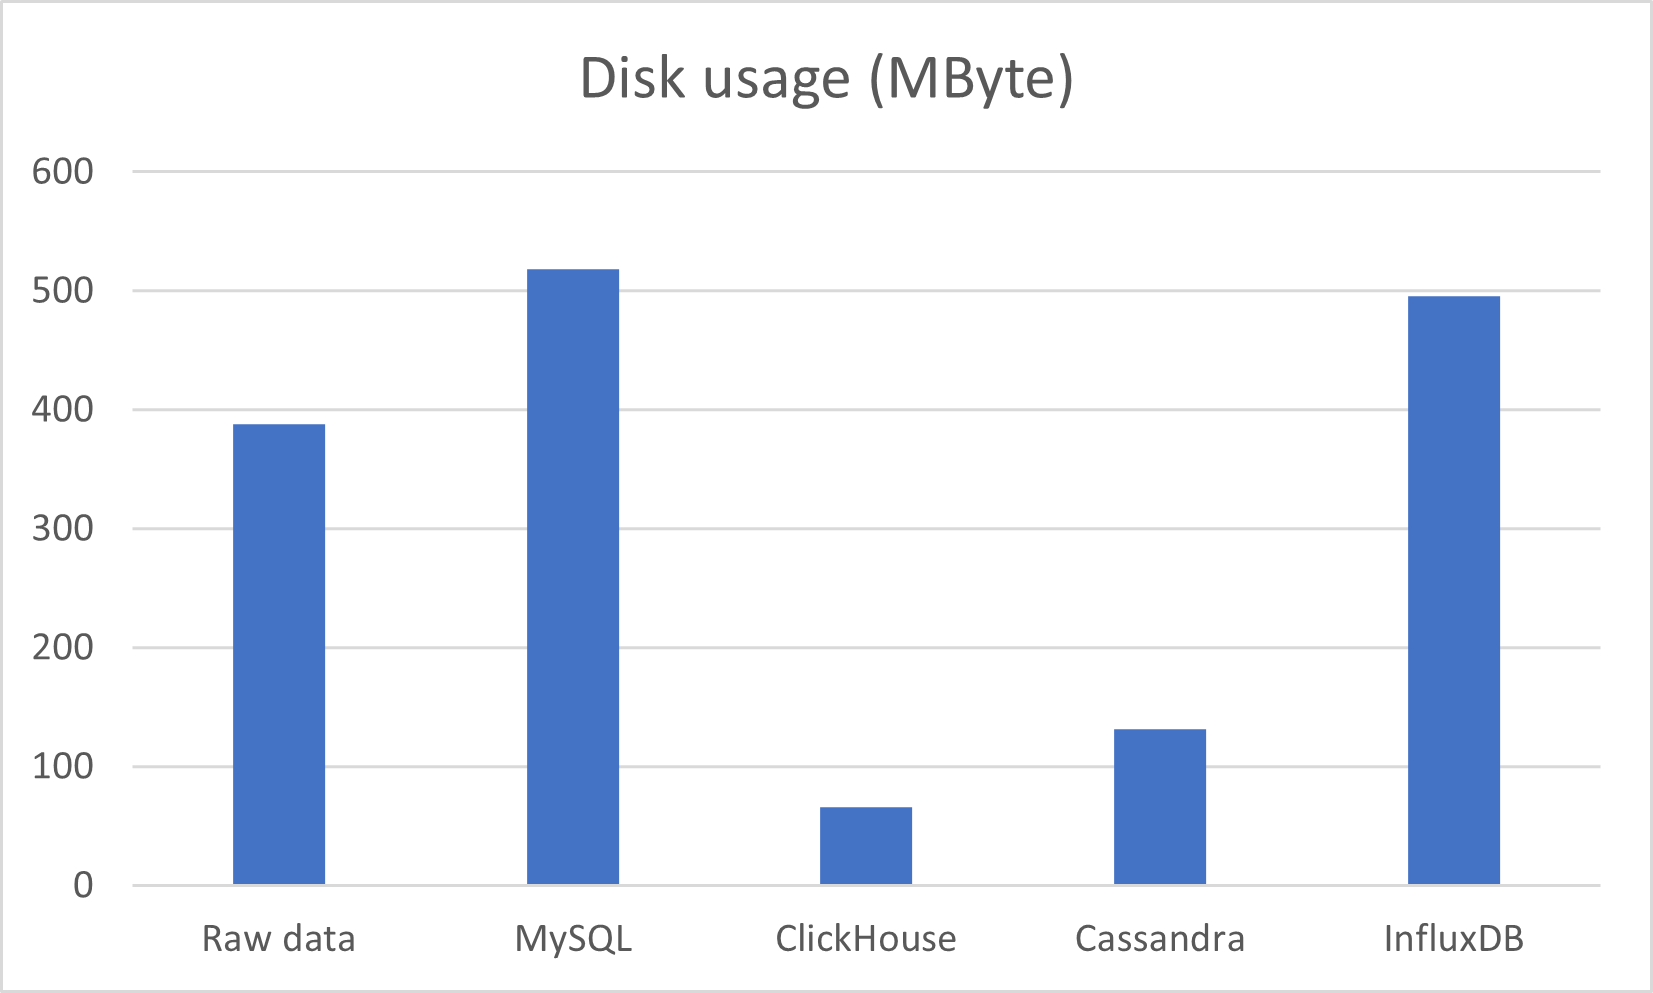
\includegraphics[width=0.9\textwidth]{gfx/disk_usage.png}
    \captionof{figure}{Disk usage of each database}
    \label{fig:disk_usage}
  \end{minipage}
  \hfill
  \begin{minipage}[b]{0.49\textwidth}
    \centering
   \begin{tabular}{@{}ll@{}}
\toprule
           & Disk usage (MByte)  \\ \midrule
Raw data   & 388.28 \\
MySQL      & 518.35 \\
ClickHouse & 66.36 \\
Cassandra  & 131.71 \\
InfluxDB   & 495.82 \\ \bottomrule
    \end{tabular}
      \captionof{table}{Disk usage}
    \end{minipage}
  \end{minipage}

From the figure \ref{fig:disk_usage}, it is concluded that the data consumes the least amount of disk space at ClickHouse at approximately 70MB, followed by Cassandra at approximately 130MB. Both of these databases consume less disk space than the original binary CAN bus data file. In contrast InfluxDB and MySQL require more space at around 500MB. As a result, ClickHouse was rated very good, Cassandra was rated good, and InfluxDB and MySQL were rated medium in terms of disk usage.

\section{Flexibility of database}
In order to work, data needs to be heavily formatted and shaped to fit into the table structure\cite{mongodb}. Especially for automotive CAN bus data, when the DBC file is changed, the corresponding table also needs to be changed, which can cause problems for developers. So Flexibility of database is also valuable and the score is 10.

MySQL, ClickHouse and Cassandra all require the structure of the tables and the data type of each column to be defined in advance. Whereas InfluxDB can accept any data type, due to the lack of a schema. While the first three databases need to redefine the table structure if certain rules in the DBC file are modified, InfluxDB does not. This significantly reduces the workload of database administrators. As a consequence, in terms of flexibility, InfluxDB was rated very good, while the rest of the databases are rated as medium.

\section{Performance Analysis}

\begin{table}[hbt!]
\centering
\resizebox{\textwidth}{!}{%
\begin{tabular}{@{}l|l|ll|ll|ll|ll@{}}
\toprule
\multirow{2}{*}{\textbf{Criteria}} &
  \multirow{2}{*}{\textbf{Weight}} &
  \multicolumn{2}{l|}{\textbf{MySQL}} &
  \multicolumn{2}{l|}{\textbf{ClickHouse}} &
  \multicolumn{2}{l|}{\textbf{Cassandra}} &
  \multicolumn{2}{l}{\textbf{InfluxDB}} \\ \cmidrule(l){3-10} 
 &
   &
  \multicolumn{1}{l|}{unweighted} &
  weighted &
  \multicolumn{1}{l|}{unweighted} &
  weighted &
  \multicolumn{1}{l|}{unweighted} &
  weighted &
  \multicolumn{1}{l|}{unweighted} &
  weighted \\ \midrule
Write performance       & 25  & \multicolumn{1}{l|}{2}  & 50  & \multicolumn{1}{l|}{5}  & 125 & \multicolumn{1}{l|}{4}  & 100 & \multicolumn{1}{l|}{3}  & 75  \\
Read performance        & 20  & \multicolumn{1}{l|}{4}  & 80  & \multicolumn{1}{l|}{5}  & 100 & \multicolumn{1}{l|}{3}  & 60  & \multicolumn{1}{l|}{2}  & 40  \\
Aggregation performance & 20  & \multicolumn{1}{l|}{3}  & 60  & \multicolumn{1}{l|}{5}  & 100 & \multicolumn{1}{l|}{2}  & 40  & \multicolumn{1}{l|}{4}  & 80  \\
Disk usage              & 25  & \multicolumn{1}{l|}{3}  & 75  & \multicolumn{1}{l|}{5}  & 125 & \multicolumn{1}{l|}{4}  & 100 & \multicolumn{1}{l|}{3}  & 75  \\
Flexibility of database & 10  & \multicolumn{1}{l|}{3}  & 30  & \multicolumn{1}{l|}{3}  & 30  & \multicolumn{1}{l|}{3}  & 30  & \multicolumn{1}{l|}{5}  & 50  \\ \midrule
\textbf{Sum}            & 100 & \multicolumn{1}{l|}{15} & 295 & \multicolumn{1}{l|}{23} & 480 & \multicolumn{1}{l|}{16} & 330 & \multicolumn{1}{l|}{17} & 320 \\ \bottomrule
\end{tabular}%
}
\caption{Result of Weighted sum mod}
\label{tab:result_lsm}
\end{table}

The final result (Table \ref{tab:result_lsm}) shows that ClickHouse has a large advantage in write performance, query performance and disk usage compared to the rest of the databases, followed by Cassandra and InfluxDB. The traditional relational database MySQL does not perform well, especially in terms of write performance. 

\paragraph{Write performance}
Obviously, the three LSM-Tree-based databases are significantly higher than the B+ tree-based MySQL in terms of write performance. As written in the previous Section \ref{lsm_bplus}, compared with B-tree, LSM-tree can significantly reduce the cost of the hard disk arm, and can provide high-speed insertion of files for a long time. In addition, MySQL's single SQL is single-threaded and can only run one core. ClickHouse, on the contrary, has as many CPUs and consumes as many resources, so write performance is better than other databases.

\paragraph{Disk Usage}
ClickHouse with column-oriented storage is significantly better than MySQL with row-oriented storage in terms of disk consumption. Wide column database Cassandra also performs well with LZ4 compression but still does not perform as well as ClickHouse. As mentioned in the previous Section \ref{row_column_storage}, the data in column-oriented database is divided into multiple independent columns for storage, and data of the same type is stored continuously together, making it easy to compress.

\paragraph{Query Performance}

Disregarding the previous SQL parsing process, this SQL can be abstracted into two simple steps:

\begin{minted}[
frame=lines,
framesep=2mm,
baselinestretch=1.2,
bgcolor=LightGray,
fontsize=\footnotesize,
linenos
]{bash}
SELECT AVG(MO_Drehzahl_01) FROM audi_a8.Motor_12;
\end{minted}


\begin{enumerate}
    \item Read the data file from disk and load it into memory
    \item Parse the data and find the average
\end{enumerate}

Assume a 3.6GHz CPU and 7200 rpm mechanical hard drive. Then the CPU takes $ 1/3.6GHz \approx 0.28ns $ to execute an instruction, and the 7200 rpm mechanical hard drive reads about 100MB per second. This means that the CPU can only theoretically read about 0.028 bytes in the time it takes for the hard drive to execute an instruction. Thus it is clear that most of the time spent on computing tasks is actually on IO. So the way in which the database reduces disk IO becomes critical.

The principle of a columnar storage database stores each column separately, reducing the amount of data loaded each time. This reduces the amount of data that is loaded each time. Suppose the data file data.bin is 1Gb in size and takes 5 seconds to load. If each column is written to a separate file, then if only the maximum vehicle speed needs to be calculated, then only the speed.bin file needs to be loaded, which is about 200MB, theoretically reducing the read time by about 80 percent. In addition, by compressing data per column, IO will be reduced even further and queries will be faster. So it is still the column database ClickHouse ahead of other databases in this area of aggregated queries.

%*****************************************
\chapter{Conclusions}
\label{ch:closure}
%*****************************************

This thesis designs a monitoring and analysis system based on big data technology for processing and storing CAN bus data. The huge amount of raw CAN bus data stored in the HDFS file system is parsed by using the Spark analytics engine, and then the parsed data is stored in the database.

By comparing different types of databases, it is concluded that column-oriented databases based on LSM-Tree storage structure are more suitable for storing and querying CAN bus data. There are three main performance test directions, namely, write performance, disk usage and query performance. ClickHouse with a pure column-oriented structure received the highest score compared to MySQL, Cassandra and InfluxDB.

The future directions of work are the following:
\begin{itemize}
    \item The whole system will be clouded. In the future, everything will run in the cloud, no matter it is a private or public cloud, and the operation and maintenance team may no longer be in contact with the real physical machine, but an isolated container.
    
    \item Future work is directed towards a fully distributed environment. The system operating environment and all test results in this thesis was done through a single node server. However, in the face of massive data, it is inevitable that the system will be deployed on several or even dozens of servers.
    
    \item CAN bus data is just a starting point. At present, vehicle bus technology is developing rapidly and vehicular Ethernet will become more and more popular. How to store vehicular Ethernet in real time will be a new challenge.
    
    \item Since CAN bus data is time-series data, an integrated time-series model (TSM) with deep recurrent neural networks (RNN) via long short-term memory (LSTM) units is used to dynamically estimate different states in the vehicle, such as battery consumption, driving habits or potential hazards.
    
\end{itemize}

